\documentclass{book}
%%% Indexed through Sect. 2.6
\usepackage{makeidx}
\usepackage{multicol}
\usepackage{times}
\usepackage{helvet}
\usepackage{courier}
\usepackage{url}
%\usepackage[final]{graphics} % for dvi and ps
\usepackage{graphicx} % for pdf
\usepackage[colorlinks=true,linkcolor=blue]{hyperref}

\makeindex

\oddsidemargin 0.5in
\evensidemargin 0in
\marginparwidth 0in
\marginparsep 0in
\textwidth 6in
\topmargin 0in
\textheight 8.5 in

\newcommand{\ct}[1]{{\ttfamily #1}} % argument set in tt type
                                    % (``computer type'')
\newcommand{\cv}[1]{{\ttfamily{\itshape #1}}} % argument set in
                                              % italic tt type
                                              % (``computer variable'') 
\newcommand{\indexct}[1]{\index{#1@\ct{#1}}} % Index a computer term
\newcommand{\indexglobal}[1]{\index{#1@\ct{*#1*}}} % Index a global variable
\newcommand{\indexsv}[1]{\index{#1@\ct{#1}!SNEPSUL variable}}
\newcommand{\docfun}[2]{\vspace{3ex}\par\noindent\ct{(#1
#2)}\indexct{#1}\newline}
\newcommand{\pathdef}[1]{\vspace{3ex}\par\noindent{\ttfamily #1}\newline}

\title{\bf SNePS~2.8 USER'S MANUAL\thanks{The development of SNePS
    was supported in part by: the National Science Foundation under
    Grants IRI-8610517 and REC-0106338; the Defense Advanced Research
    Projects Agency under Contract F30602-87-C-0136 (monitored by the
    Rome Air Development Center) to the Calspan-UB Research Center;
    the Air Force Systems Command, Rome Air Development Center,
    Griffiss Air Force Base, New York 13441-5700, and the Air Force
    Office of Scientific Research, Bolling AFB DC 20332 under Contract
    No.  F30602-85-C-0008, which supported the Northeast Artificial
    Intelligence Consortium (NAIC); NASA under contract NAS 9-19335 to
    Amherst Systems, Inc.; ONR under contract N00014-98-C-0062 to
    Apple Aid, Inc.; the U.S. Army CECOM Intelligence and Information
    Warfare Directorate (I2WD) through a contract with CACI
    Technologies and through Contract \#DAAB-07-01-D-G001 with
    Booze$\cdot$Allen \& Hamilton; and CUBRC under prime contract
    FA8750-06-C-0184 between CUBRC and U.S. Air Force Research
    Laboratory, Rome, NY.}\\
}

\author{ \bf
Stuart C. Shapiro \\ \bf
and \\ \bf
The SNePS Implementation Group \\[2ex] \bf
Department of Computer Science and Engineering\\ \bf
University at Buffalo, The State University of New York\\ \bf
201 Bell Hall\\ \bf
Buffalo, NY 14260-2000 \\[2ex] \bf
\date{\today}}


\begin{document}
\frontmatter
\maketitle

\pagebreak
Over the years, many people have contributed to the design and
implementation of SNePS, and to the writing of successive versions of
the SNePS User's Manual.  They constitute ``The SNePS Implementation
Group'' cited on the title page, and I am grateful to them.  They are
listed here.  If I have inadvertently omitted anyone's name, or have
mispelled anyone's name, please let me know, and I will correct it for
the next printing of this Manual.
\begin{multicols}{3}
\noindent Syed S. Ali\\
Michael J. Almeida\\
Charles W. Arnold\\
Robert J. Bechtel\\
Sudhaka Bharadwaj\\
Jong S. Byoun\\
Alistair E. Campbell\\
Scott S. Campbell\\
Hans Chalupsky\\
Chung M. Chan\\
Joongmin Choi\\
Chi C. Choy\\
Soon Ae Chun\\
Maria R. Cravo\\
Dmitriy Dligach\\
Zuzana Dobes\\
Gerard F. Donlon\\
Nicholas E. Eastridge\\
Elissa Feit\\
Ari I. Fogel\\
David Forster\\
Richard B. Fritzson\\
James Geller\\
Susan M. Haller\\
Richard G. Hull\\
Haythem Ismail\\
Frances L Johnson\\
Steven D. Johnson\\
Darrel L. Joy\\
Sudha Kailar\\
Michael W. Kandefer\\
Deepak Kumar\\
Stanley C. Kwasny\\
John S. Lewocz\\
Naicong Li\\
John D. Lowrance\\
Christopher Lusardi\\
Aya Saif El-yazal Mahfouz\\
Anthony S. Maida\\
Mark D. Malamut\\
Nuno Mamede\\
Jo\~{a}o P. Martins\\
Pedro A. Matos\\
Donald P. McKay\\
James P. McKew\\
Ernesto J. Morgado\\
William A. Neagle\\
Jeannette G. Neal\\
Jane Terry Nutter\\
Rafail Ostrovsky\\
Sandra L. Peters\\
Carlos Pinto-Ferreira\\
William J. Rapaport\\
Victor H. Saks\\
Harold L. Shubin\\
Reid G. Simmons\\
Benjamin R. Spigle, Jr.\\
Rohini K. Srihari\\
William M. Stanton\\
Jennifer M. Suchin\\
Lynn M. Tranchell\\
Jason C. Van Blargan\\
Nicholas F. Vitulli\\
Diana K. Webster\\
Janyce M. Wiebe\\
Albert Hanyong Yuhan\\
Martin J. Zaidel
\end{multicols}

\begin{flushright}
Stuart C. Shapiro
\end{flushright}

\tableofcontents

\cleardoublepage
\addcontentsline{toc}{chapter}{List of Figures}
\listoffigures

\mainmatter
\chapter{Introduction}
\section{General}

SNePS is a logic-, frame- and network-based knowledge representation,
reasoning and acting system.  The name ``SNePS'' originally was an
acronym of ``The Semantic Network Processing System,''.

A semantic network, roughly speaking, is a labeled directed graph in which nodes
represent entities, arc labels represent binary relations, and an arc labeled
$R$ going from node $n$ to node $m$ represents the fact that the entity
represented by $n$ bears the relation represented by $R$ to the entity
represented by $m$.  The set of nodes in the network-based view of SNePS is
coextensive with the set of terms in the logic-based view of SNePS.

SNePS is called a {\em propositional} semantic network because every proposition
represented in the network is represented by a node, not by an arc.  Relations
represented by arcs may be thought of as part of the syntactic structure of the
node they emanate from.  In the frame-based view of SNePS, every non-atomic term
is a frame whose slots are the arcs of the network-based view, and the fillers
of the slots are the nodes those arcs point to.  Whenever information is added
to the network, it is added in the form of a frame---a node with arcs (slots)
emanating from it to other nodes (the slot fillers).

Each entity represented in the network is represented by a unique node/term.
This is enforced by SNePS~2 in that whenever the user specifies a node to be
added to the network that would look exactly like one already there, in the
sense of having the same set of arcs (slots) going from it to the same set of
other nodes (fillers), SNePS~2 retrieves the old one instead of building the new
one.

SNePSUL, the SNePS User Language, is the lowest-level command language
for using SNePS.  It is a Lispish language, usually entered by the
user at the top-level SNePSUL read-eval-print loop, but it can also be
called from Lisp code or from GATN arcs.  The SNePSUL chapters of this
manual follow the style of Guy Steele's {\sc Common Lisp} book, and
assume that the reader is familiar with that book and with {\sc Common
  Lisp.}  The organization of this manual has been retained from the
time when SNePSUL was the standard way to interact with SNePS.
However, the use of SNePSLOG is now recommended.

SNIP (Chapter~\ref{snipchap}), the SNePS Inference Package, interprets
certain nodes as representing reasoning rules, called {\em deduction
rules}.  SNIP supports a variety of specially designed propositional
connectives and quantifiers, and performs a kind of combined
forward/backward inference called {\em bi-directional} inference.

SNePSLOG (Chapter~\ref{snepslogchap}) is a logic programming interface
to SNePS, and provides direct access in a predicate logic notation to
almost all the facilities provided by SNePSUL.  It is now the
recommended way to interact with SNePS.

SNeBR (Chapter~\ref{snebrchap}), the SNePS Belief Revision system,
recognizes when a contradiction exists in the network, identifies
possible culprits, and performs disbelief propagation.  It eliminates
contradictions automatically in some cases, and helps the user to do
so in the general case.

SNaLPS (Chapter~\ref{snalpschap}), the SNePS Natural Language
Processing System, consists of a morphological analyzer, a
morphological synthesizer, and a Generalized Augmented Transition
Network (GATN) Grammar interpreter/compiler.  Using these facilities,
one can write natural language (and other) interfaces for SNePS.


\section{What's New}
\label{sec:whatsnew}
\begin{description}
\item[SNePS~2] differs in several respects from its predecessor, now called
SNePS-79, mostly because of theoretical decisions that were made since
SNePS-79 was implemented.

\item[SNePS~2.1] differs from SNePS~2.0 by including belief revision as a
standard feature.

\item[SNePS~2.3] includes some techniques for making node-based inference
faster, and includes SNeRE (Chapter~\ref{snerechap}).

\item[SNePS~2.4] includes: a change in how contexts and sets of contexts are
implemented that should improve the speed of the system;
\ct{deducetrue}\indexct{deducetrue},
\ct{deducefalse}\indexct{deducefalse},
\ct{deducewh}\indexct{deducewh}, and
\ct{deducewhnot}\indexct{deducewhnot} (Section~\ref{retrievsec}); the
Tell-Ask interface (Section~\ref {sec:tellask}); and SNePSLOG Mode 3,
which allows SNePSLOG syntax to be used to build SNePS networks using
as flexible a choice of relations as may be done using SNePSUL syntax
(Section~\ref{snepslogcommands}).

\item[SNePS~2.5]includes: a change in how nodes are implemented and how
  sets of nodes are ordered that should improve the speed of the system;
\ct{activate}\indexct{activate} (Section~\ref{build-sec});
the SNePSLOG \texttt{perform} command
(Section~\ref{snepslogcommands});
a revised semantics for \ct{when-do}, with the old \ct{when-do} now
renamed \ct{whenever-do} (Section~\ref{acting-sect}).

\item[SNePS~2.6] code has been modified so that it can be loaded into
  \textsc{Allegro CL} version 6.X and used with its default case mode
  of ``case-sensitive-lower'' (all predefined \textsc{Common Lisp}
  symbols have lower-case names, and the case of characters typed into
  the \textsc{Lisp} listener is left as originally typed) \textbf{or}
  loaded into earlier versions of \textsc{Allegro CL}, or other
  versions of \textsc{Common Lisp} that use ``case-insensitive-upper''
  mode (all predefined \textsc{Common Lisp} symbols have upper-case
  names, and the case of characters typed into the \textsc{Lisp}
  listener is changed to upper case).  Some SNePS symbols may look
  different in the two different modes, such as \texttt{M1}
  vs. \texttt{m1}. The output for the examples in this manual was generated from earlier versions of SNePS, so it is typically in uppercase (except where special formatting was used to generate the output).
  
\item[SNePS~2.6.1]
Previously, the functions \texttt{+}\indexct{+} and
  \texttt{\&}\indexct{\&} took only two arguments.  Now they can take
  zero or more.  The function \texttt{show}\indexct{show} has been
  added.  The SNeRE mental action \texttt{believe}\indexct{believe}
  now checks for and \texttt{disbelieve}s\indexct{disbelieve} more
  contradictory beliefs than before.  The SNePSLOG commands
  \texttt{activate}\indexct{activate},
  \texttt{activate!}\index{activate"!@\ct{activate"!}},
  \texttt{ask}\indexct{ask}, \texttt{askifnot}\indexct{askifnot},
  \texttt{askwh}\indexct{askwh}, and
  \texttt{askwhnot}\indexct{askwhnot} have been added.  There have
  been several other bug fixes.  Documentation of the SNePSLOG command
  {\tt list-wffs} \indexct{list-wffs} has been added to the manual; it
  was previously available.  Section~\ref{snepslogsnere:sec}, ``SNeRE
  in SNePSLOG,'' has been added to this manual, some material
  describing features that were never implemented in SNePS~2 has been
  deleted from the manual, and there have been other editorial
  changes.  A complete description of what's new in SNePS~2.6.1 is at
  \url{http://www.cse.buffalo.edu/sneps/Downloads/releaseNotes261.html}.
  
\item[SNePS~2.7] The SNePSLOG parser has been completely rewritten,
  improved, and made more robust.  The chapter on SNePSLOG has been
  completely rewritten.  SNePSLOG is now the preferred interface to
  SNePS.  Normal output from SNePSLOG now shows the wffName.  The
  SNePSLOG command \texttt{define-terms} has been added, and
  \texttt{define-frame} given an optional string argument, which, when
  used together, provide a facility for giving a natural language
  gloss of SNePS terms.  The tell-ask interface has been improved, and
  its documentation has been moved to \S\ref{sec:tellask}.  Previously
  \texttt{askwh} and \texttt{askwhnot} would return a simple list of
  terms, even if the query had more than one free variable. Now, they
  return a list of substitutions even if the query has only one free
  variable.  (Similarly for the SNePSUL commands \texttt{deducewh} and
  \texttt{deducewhnot}).  A Java-SNePS API has been added to give Java
  programs access to SNePS via the tell-ask interface, see
  \S\ref{sec:api}.  The final cases in which the inference system
  could get into infinite recursion have been eliminated---see
  \S\ref{snepsulrec:sec} and \S\ref{snepslogrec:sec}.  The SNePSUL
  \texttt{intext} command and the new SNePSLOG \texttt{load} command
  silently load files.  Previously, one could not have a node named
  with a string the Lisp reader could not handle, such as
  \texttt{"\#"}, and \texttt{node-to-lisp-object} did not handle nodes
  with names like \texttt{"5 pounds"}. Both these problems are now
  fixed. A node's name can now be any Lisp number, string, or symbol,
  and \texttt{node-to-lisp-object} is able to handle it.  Previously,
  inference and acting tracing was on by default, now they are off by
  default.  Previously, in \texttt{add-to-context}, only the wffs in
  termSet that had already been introduced to the KB as hypotheses
  were added as hypotheses of the context. Now, all the wffs listed as
  to be added are asserted into the context.  An procedural attachment
  facility has been added.  It is described in
  Chapter~\ref{attachproc:chap}.  The guarded acts in \texttt{snif}
  and \texttt{sniterate} can now take sets of conditions and sets of
  acts. \texttt{snif} and each loop of \texttt{sniterate} still
  performs one act one of whose guards holds.  The mental acts
  \texttt{adopt} and \texttt{unadopt} are now available for adopting
  and unadopting policies, and should be used for those purposes
  instead of \texttt{believe} and \texttt{disbelieve}.  A chapter on
  SNeBR (Chapter~\ref{snebrchap}) has been added.  XGinseng has been
  eliminated because it was implemented in Garnet, which has not been
  maintained, and was difficult to use.  SNePS networks may now be
  displayed by \texttt{show}\indexct{show}, either via:
  \texttt{dot}\indexct{dot}; or \texttt{JUNG}\indexct{JUNG} and
  \texttt{JIMI}\indexct{JIMI}, depending on the installers choice
  (both require separate downloading).  If both versions are
  installed, the user may choose which one to use by setting the value
  of the global variable
  \texttt{cl-user:*use-gui-show*}\index{use-gui-show@\ct{cl-user:*use-gui-show*}}.
  
  There have been other bug fixes, improvements to speed, and
  improvements to user messages.  A complete description of what's new
  in SNePS~2.7 is at
  \url{http://www.cse.buffalo.edu/sneps/Downloads/releaseNotes262.html}.

\item[SNePS~2.7.1]\mbox{}
  \begin{description}
\item[SNePS]\mbox{}\\
The command \texttt{(beliefs-about \{{\it nodeset}\}*
{\it context-specifier})} has been added.  It returns a set of
all the nodes, asserted in the given context, that dominate the nodes
described by the \texttt{{\it nodeset}}s.

\item[SNePSLOG]\mbox{}
\begin{enumerate}

\item In SNePS 2.7.0, an attempt to use the \texttt{\&=>}-Introduction rule
  caused a Lisp error.  That has been fixed, and \texttt{\&=>}-Introduction
  works in SNePS 2.7.1.

\item In SNePS 2.7.0, the \texttt{v=>}-Introduction rule did not work.
  Moreover, the \texttt{v=>}-Introduction rule, as documented in the
  \textit{SNePS 2.7 User's Manual} is incorrect.  In SnePS 2.7.1, the
    \texttt{v=>}-Introduction rule works as long as there is only a single
    antecedent.  The \texttt{v=>}-Introduction rule for multiple antecedents is
    not yet implemented.

\item In certain circumstances, \texttt{activate} and
\texttt{activate!} caused an error.  That has been fixed.

\item  The snepslogCommand \texttt{beliefs-about pTermSet [.]} has
been added.  It returns a set of all the asserted wffs that dominate
the terms described by \texttt{pTermSet}.

\item  The function \texttt{(nl-tell {\it string})} has been added.  It may
	      be called from the top-level Lisp listener in the
	      \texttt{snepslog} package.  Assuming that a lexicon and GATN
	      grammar have been loaded, \texttt{nl-tell} passes
	      \texttt{{\it string}} to the parser, and returns a string
	      containing whatever the parser returns.

            \item Linebreaks may occur in input to the SNePSLOG reader, but if
              the input looks like it might end prematurely, the character
              ``\verb.\.'' (without the quotation marks) may be placed before
                the end-of-line to indicate that the input continues on the next
                line.  For example, the wff \texttt{p() => q().} may end just
                before the \texttt{=>} if and only if the line with \texttt{p()}
                ends with a ``\verb.\.''.  This is also very useful in a
                  \texttt{define-frame} command if you want to put the
                  documentation string on the next line.  Previously, this was
                  an undocumented feature, but ``\texttt{-}'' was used instead
                  of ``\verb.\.'', which caused problems if a linebreak
                    occurred in a path just after a converse relation, like
                    \texttt{subclass-}.
                    
\item  SNePSLOG now allows the use of \texttt{and}, \texttt{or},
     \texttt{nand}, \texttt{nor}, \texttt{xor}, and
     \texttt{iff}, each followed by a termSet.  For example,
     \texttt{all(x)(Entity(x) => xor\{Animal(x), Vegetable(x),
     Mineral(x)\})}.
\end{enumerate}

\item[SNIP]\mbox{}
\begin{enumerate}

\item In certain circumstances, \texttt{activate} caused an error.
That has been fixed.

\item See the note about \texttt{\&=>}-Introduction under SNePSLOG, above.

\item  See the note about \texttt{v=>}-Introduction under SNePSLOG, above.
\end{enumerate}

\item[SNeBR]\mbox{}\\
Restriction sets in node supports and in contexts have been
eliminated in favor of a global set of minimal nogoods.  A minimal
nogood is a set of hypotheses that is known to be inconsistent, such
that no subset of it is known to be inconsistent.

\item[SNeRE]\mbox{}
\begin{enumerate}
\item  Consider the following knowledge base:
\begin{quote}
\begin{verbatim}
: andor(1,1){aheadIs(wall), aheadIs(corridor)}.
  wff3!:  andor(1,1){aheadIs(corridor),aheadIs(wall)}    

: andor(1,1){holding(person), holding(noOne)}.
  wff6!:  andor(1,1){holding(noOne),holding(person)}    

: holding(noOne).
  wff5!:  holding(noOne)    

: aheadIs(corridor).
  wff2!:  aheadIs(corridor)    
\end{verbatim}
\end{quote}
Now, ask a question whose answer looks like a state constraint.
\begin{quote}
\begin{verbatim}
: (holding(noOne) and aheadIs(wall))?
  wff9!:  andor(0,1){holding(noOne),aheadIs(wall)}
             {<der,{wff2,wff3},{}>}  
\end{verbatim}
\end{quote}
If we now do
\begin{quote}
\begin{verbatim}
: perform believe(aheadIs(wall))
\end{verbatim}
\end{quote}
In SNePS 2.7.0, \texttt{holding(noOne)} would no longer be asserted, even though
\texttt{wff9} will no longer be asserted once \texttt{wff2} is
disbelieved. This is fixed in SNePS 2.7.1.
\end{enumerate}
  \end{description}
SNePS 2.7.1 also includes some additional improvements.

\item[SNePS~2.8]\mbox{}
  \begin{description}
  \item[SNePS]\mbox{}
    \begin{enumerate}
    \item SNePS can now be compiled by Armed Bear Common Lisp (ABCL), which
       produces Java bytecode.
     \item Nodes whose identifiers are not readable by Lisp as symbols
       (e.g. numbers and identifiers with spaces in them) are now printed with
       escape brackets.
     \item When typing nodes, a user may use the escape character and escape
       brackets.
    \end{enumerate}

  \item[SNePSLOG]\mbox{}
\begin{enumerate}
\item In version 2.7.1, if an atomic symbol (individual constant, function
  symbol, etc.) began with a substring that matched any of the following:
  \texttt{and}, \texttt{or}, \texttt{nand}, \texttt{nor}, \texttt{xor},
  \texttt{iff}, \texttt{andor}, \texttt{thresh}, or \texttt{nexists} it would be
  misparsed, or an error would result.  For example, \texttt{instanceOf(north,
    direction)} would be parsed as\\ \texttt{instanceOf($\sim$th, direction)}.  That
  has now been fixed.  However, now none of these connectives may immediately be
  followed by a blank, but must immediately be followed either by
  ``\texttt{\{}'' or "\texttt{(}'', whichever is appropriate.

\item \texttt{tell} has been given optional format arguments.  So instead
     of evaluating
     \begin{quote}
     \texttt{(tell (format nil "\texttt{$\sim$A($\sim$A).}" 'Dog 'Fido))}
     \end{quote}
     you may now do
     \begin{quote}
     \texttt{(tell "\texttt{$\sim$A($\sim$A).}" 'Dog 'Fido)}
     \end{quote}

   \item The character ``!'' is now optional at the end of a wffname.  If the
     ``!''  is not the terminal character of the wffNameCommand (that is, is not
     the final character of the SNePSLOG command), it will be ignored.

   \item The macro \texttt{(foreachsub \textit{variables subs} \&body
       \textit{forms})} has been added to the tell/ask interface.  For each
     substitution in \cv{subs}, \texttt{foreachsub} evaluates the forms in
     \cv{forms} with the variables in \cv{variables} taking on the
     values specified by that substitution.  This is particularly useful for
     processing the values returned by \texttt{(askwh ...)}  or by \texttt{(tell
       "askwh...")}.
   \item Individual constants whose identifiers are not readable by Lisp as
     symbols (e.g. numbers and strings with spaces in them) are now printed with
     escape brackets.
   \item The SNePSLOG parser can read individual constants containing the escape
     character and escape brackets.
   \item The \texttt{show} command now displays molecular nodes using their wff
     names.
   \item The attempt to assert a negated, universally quantified \texttt{andor}
     or \texttt{thresh}, such as\\
     \verb|~|\texttt{(all(x)(B(a,x) <=> x))} previously
     caused an error.  This has been fixed.
    \end{enumerate}

  \item[SNIP]\mbox{}
    \begin{enumerate}
    \item Before if \texttt{p(a)} were an hypothesis of the current context, and
      \texttt{p(a)|-r(a)}, then \texttt{p(a)=>r(a)} would not be inferred
      because SNIP didn't think that \texttt{p(a)} was introduced in the
      hypothetical context.  That has now been fixed.
    \end{enumerate}

  \item[SNeBR]\mbox{}
    \begin{enumerate}
    \item SNeBR has been greatly improved.  Previously, SNeBR performed manual
      nonprioritized belief revision in most cases, and automatic prioritized
      belief revision when a new belief was added by the \texttt{believe} act,
      but then only with direct contradictions between hypotheses.  Now, the
      user can independently specify prioritized \emph{vs.}\ nonprioritized and
      manual (now called ``assisted'') \emph{vs.}\ automatic belief revision, and
      derived contradictions triggered by \texttt{believe} are recognized and
      handled.  The user can also specify what epistemic entrenchment ordering
      function the system is to use during automatic belief revision.  Several
      such ordering functions are supplied, and the user can define others.  For
      the details, see Chapter~\ref{snebrchap} of this Manual.
    \end{enumerate}
  \end{description}
SNePS 2.8 also includes some additional improvements.
\end{description}


% ALTERED 7/2002 BY FLJ
\section{System Portability}
SNePS~2 is written in ANSI {\sc Common Lisp} (two exceptions are noted
in the following paragraph). Hence, every proper implementation of
ANSI {\sc Common Lisp} should be sufficient to run SNePS~2.  In
particular, SNePS~2 should run successfully using the following:
\begin{itemize}
\item UNIX operating system
\item LINUX operating system
\item Apple/Macintosh operating system
\item Microsoft Windows operating system
\item Allegro Common Lisp (Franz Inc.)
\item Lucid (or Sun) Common Lisp
\item GNU CLISP
\item CMU Common Lisp
\item Macintosh Common Lisp
\item Harlequin LispWorks
\item Armed Bear Common Lisp (ABCL)
\end{itemize}
%Previous versions of SNePS ran successfully (or were reported to run)
%using the following platforms/systems --- hence, there is a
%significant chance that the current version will run too (or will
%require only minor modifications to make it run):  
%\begin{itemize}
%\item VAX/VMS operating system
%\item Texas Instruments Explorer
%\item Kyoto Common Lisp 
%\item VAX Common Lisp
%\item AKCL 
%\end{itemize}

The \texttt{JUNG/JIMI}\indexct{JUNG}\indexct{JIMI} version of
\texttt{show}\indexct{show}, and the Java-SNePS API\index{Java-SNePS API}
 require some facilities peculiar to Franz's ACL\index{Franz ACL}.
For installations that do not have that compiler, an executable file
is available for downloading from
\url{http://www.cse.buffalo.edu/sneps/Downloads/}. That executable
provides all the features of SNePS~2.8.  Every other feature of
SNePS~2.8 is written in ANSI Common Lisp.

\section{Commands and Environments}\label{environsect}


A SNePSUL {\em command}\index{commands!SNEPSUL} is classified
according to its role either as a {\em procedure}\index{procedure,
SNEPSUL} or as a {\em function}\index{function, SNEPSUL}.  A {\em
procedure} is a command that performs some action but returns nothing,
using the {\sc Common Lisp} {\tt (values)} function.  A {\em function}
is a command that always returns some value, possibly after having
performed some action as a side effect. A function is implemented
directly as a Lisp function.

A command is also classified according to the environment(s) in which
it may legally appear.  A procedure can be entered only at the top
level of SNePSUL.  A function, however, may appear in many different
environments.  The five environments are:
\begin{enumerate}
\item The top level of SNePS~2
\item A {\em relation-set} position embedded in a command
\item A {\em node-set} position in {\tt build}\indexct{build}
\item A {\em node-set} position in {\tt find}\indexct{find} or {\tt
findassert}\indexct{findassert}
\item A {\em node-set} position in any of the other commands
\end{enumerate}

Finally, a command can be classified according to the relation between its
position and the position of its arguments in the input line.

Most commands have an arbitrary number of arguments. They are called {\em
prefix commands}\index{commands!prefix}, because they can only be
entered using Cambridge prefix
notation:
\begin{center}
({\em prefix-command argument \ldots argument}).
\end{center}

Some two-argument commands can be entered in infix position, and so
are called {\em infix commands}\index{commands!infix}.  When an infix
command is used in infix position, SNePS rearranges the input line to
transform the form into a prefix form.  Precedence is always from left
to right. An infix command can be used as
\begin{center}
({\em infix-command argument argument})
\end{center}
or as
\begin{center}
{\em argument infix-command argument}
\end{center}
with no parentheses.

Since SNePS always remembers the result of the last top-level function, an
infix command can also be used as
\begin{center}
{\em infix-command argument}
\end{center}
in which case SNePS recalls the result of the last function and makes it the
first argument for the infix command before rearranging the form to the prefix
notation.

Similarly, some one-argument commands can be entered in postfix position and
therefore are called {\em postfix commands}\index{commands!postfix}.
A postfix command can be used as
\begin{center}
({\em postfix-command argument}) 
\end{center}
or as
\begin{center} \em
argument postfix-command
\end{center}
with no parentheses, or just as
\begin{center} \em
postfix-command
\end{center}
in which case the result of the last function is used as argument.

Another kind of one-argument command, called {\em macro
commands}\index{commands!macro}, have one-character names and are used
as
\begin{center}
{\em macro-command argument}
\end{center}
with no parentheses, and preferably with no space between the command
and the argument. Before passing it to the evaluator, the SNePS reader 
expands this form to a standard Cambridge prefix form.

\section{Types of Nodes}\label{sec:nodeTypes}
There are four types of nodes\index{nodes!types of} in the SNePS
network: base, variable, molecular, and pattern.

Base nodes\index{nodes!base} are distinguished by having no arcs
emanating from them.  A base node may be created by the user's
referring to it by name in the proper context.  In such a case, the
name of a base node can be any Lisp symbol.  If a number is used, the
node's name is a symbol whose symbol-name is a string of the
characters that makes up the number.  If a string is used, the node's
name is the symbol whose symbol-name is that string.  A base node may
also be created using the {\tt \#}\indexct{\#} macro command, in which
case the node's name is {\tt B}{\em x}, where $x$ is some integer.  A
base node is assumed to represent some entity---individual, object,
class, property, etc.  It is assumed that no two base nodes represent
the same, identical entity.  One may, of course, introduce an equality
or equivalence relation and the rules for using them.  In that case
the introduced equality or equivalence relation is weaker than the
identity relation just referred to.  This is the most basic way that
SNePS assumes an intensional representation---no two nodes are
intensionally identical even though they might be extensionally
equivalent.

Variable nodes\index{nodes!variable} also have no arcs emanating from
them, but represent arbitrary individuals or propositions, in much the
same way that logical variables do.  Variable nodes are created using
the {\tt \$}\indexct{\$} macro command.  The name of a variable node
is {\tt V}{\em x}, where $x$ is some number.

Molecular nodes\index{nodes!molecular} and pattern
nodes\index{nodes!pattern} have arcs emanating from them.  Molecular
nodes may represent propositions, including rules, or ``structured
individuals.''  A molecular node that represents a proposition may be
{\em asserted}\index{nodes!asserted} or {\em
unasserted}\index{nodes!unasserted}.  Pattern nodes represent
arbitrary propositions or arbitrary structured individuals, and are
similar to open sentences in predicate logic.  Pattern nodes and
unasserted molecular nodes are created by the {\tt
build}\indexct{build} function.  Asserted molecular nodes are created
by the {\tt assert}\indexct{assert} function.  An unasserted molecular
node may be asserted by using the {\tt !}\index{"!@\ct{"!}} postfix
command.  The name of a pattern node is {\tt P}{\em x}, where $x$ is a
number.  The name of a molecular node is {\tt M}{\em x}, where $x$ is
a number.  The name of an asserted molecular node is printed with a
suffix of {\tt !}\index{"!@\ct{"!}}.

Once any node is created, it may be referred to by its name.  It is
not necessary to include the {\tt !}\index{"!@\ct{"!}} suffix to refer
to an asserted molecular node.  In fact, its use is always interpreted
as a call to the {\tt !}  command, which will assert the node even if
it wasn't previously asserted.

\section{Contexts}\label{contextchap}

A {\em context}\index{contexts} is a structure with three components: 1)~a set
of hypotheses; 2)~a set of names; 3)~a kinconsistent flag.  The set of
hypotheses\index{hypotheses} is a set of nodes which are the assumptions of the
context.  The set of hypotheses is the determining component of the context in
the sense that no two contexts will have the same set of hypotheses.  The set of
names\index{contexts!names} is a set of symbols each of which functions as a
name of this context.  The kinconsistent flag\index{kinconsistent} is True if
this set of hypotheses is known to be inconsistent.

A context name\index{contexts!names} intensionally defines a
context\index{contexts!intensionally defined}, which is extensionally
defined\index{contexts!extensionally defined} by its set of
hypotheses.  The SNePSUL user always refers to contexts by
name\index{contexts!names}, and may add assertions to, or remove
assertions from a context.  Actually, such changes do not change
contexts (extensionally defined), but change the context that the name
refers to.  The system takes care of such details, and the SNePSUL
user may normally think of a context name as always referring to the
same context.

The user is always working in a particular context, called the {\em
current context}\index{context!current}.  The current context for a
particular SNePSUL command may be specified by an optional argument to
the command.  Otherwise, all commands are carried out with the {\em
default context}\index{context!default} as current context.  By
default, this context is named
\ct{default-defaultct}\indexct{default-defaultct}.

In SNePS~2.3 and later versions, a proposition
node\index{nodes!proposition} is not simply
asserted\index{nodes!asserted} or
unasserted\index{nodes!unasserted}---it is either asserted or
unasserted in each context.  The \ct{!}\index{"!@\ct{"!}} suffix will
be printed with a node's name when that node is asserted in the
current context.  An {\em hypothesis}\index{hypotheses} is a node that
was asserted by the user using \ct{assert}\indexct{assert} or
\ct{!}\index{"!@\ct{"!}}, rather than being asserted only because it
was derived during inference.  An hypothesis\index{hypotheses} is
always an hypothesis of one or more context; it may also be asserted
in other contexts, and might be unasserted in still other contexts.

Every node\index{nodes!in contexts} is said to be {\em in} zero or
more contexts\index{contexts!nodes in}.  A node $n$ is in a context
$c$ in any of the following cases:
\begin{itemize}

\item $n$ is one of the hypotheses that define $c$.

\item $n$ has been derived from a set of assumptions that is a subset of the set of hypotheses of $c$.

\item $n$ is dominated by a node in $c$.

\end{itemize}

\section{SNePSUL Variables}\label{variablessect}
SNePSUL, the SNePS User Language, has
variables\index{variables!SNEPSUL} which are entirely distinct from
SNePS variable nodes.  The value of a SNePSUL variable is always a set
of objects, {\tt nil} if nothing else.  A SNePSUL variable may be
given a value with the \ct{?}\indexct{?}, \ct{\#}\indexct{\#}, or
\ct{\$}\indexct{\$} macro commands, or with the \ct{=}\indexct{=}
infix command.  The value of a SNePSUL variable is obtained by using
the \ct{*}\indexct{*} macro command.  SNePSUL variables created and
maintained by SNePS are:
\begin{center}
\begin{tabular}{ll}
\tt nodes\indexsv{nodes}&The set of all nodes in the network. \\
\tt assertions\indexsv{assertions}&The set of all nodes in the network that were asserted by the user. \\
\tt patterns\indexsv{patterns}&The set of all pattern nodes in the network. \\
\tt varnodes\indexsv{varnodes}&The set of variable nodes in the network.\\
\tt relations\index{relations@\ct{relations}!SNEPSUL variable}
&The set of defined arc labels. \\
\tt variables\indexsv{variables}&The set of SNePSUL variables. \\
\tt defaultct\indexsv{defaultct}&The name of the default context. \\
\\
\tt commands\index{commandsa@\ct{commands}!SNEPSUL variable}&The set of SNePSUL commands. \\
\tt topcommands\indexsv{topcommands}&The set of commands valid at SNePS top-level. \\
\tt bnscommands\indexsv{bnscommands}&The set of commands valid at node-set positions in build-type commands. \\
\tt fnscommands\indexsv{fnscommands}&The set of commands valid at node-set positions in find-type commands. \\
\tt rscommands\indexsv{rscommands}&The set of commands valid at relation-set positions in commands. \\
\tt nscommands\indexsv{nscommands}&The set of commands valid at at node-set positions in other commands.
\end{tabular}
\end{center}

\chapter{SNePSUL Commands}

\section{Context Specifiers}

In a number of commands described in this chapter, part of the syntax
is {\it context-specifier}\index{context-specifier}, and the semantics
mentions the context specified by {\it context-specifier}.  In every
such case, the possible syntax of {\it context-specifier}, and what
context is specified by each possibility is:
\begin{description}

\item[{\it omit}] If the {\it context-specifier} is omitted, the
specified context is the default context (the value of {\tt
*defaultct}\indexsv{defaultct}).

\item [{\tt :context}\index{context@\ct{:context}}] The context
specified is the default context (the value of {\tt *defaultct}).

\item [{\tt :context} {\it context-name}] The context specified is
that named {\it context-name}, which must be a symbol.

\item [{\tt :context} {\it nodeset context-name}] The context
specified is that named {\it context-name}, which is initialized to be
the context whose set of hypotheses is the value of {\it nodeset},
which must be a SNePSUL expression that evaluates to a set of
proposition nodes.

\item [{\tt :context all-hyps}\indexct{all-hyps}] The context
specified is the one whose set of hypotheses is the set of all
hypotheses---all assertions entered by the user.

\end{description}

\section{Loading SNePS}

Ask whoever maintains SNePS at your site how to load SNePS.
Typically, this involves running {\sc Common Lisp,} and then loading
SNePS.

\section{Entering and Leaving SNePS}

The commands in this section move the user between the SNePSUL
evaluator and the {\sc Common Lisp} evaluator.  Although every SNePSUL
function is a {\sc Common Lisp} function, the SNePSUL loop provides certain
special facilities, so it is best to be in the proper top-level loop
for extended work.

\docfun{sneps}{}
Lisp function that brings the user into the SNePS read-eval-print loop.

\docfun{lisp}{}
SNePSUL function that returns the user to the Lisp evaluator.

\vspace{3ex}\par\noindent \ct{\^{~}}\index{\_\_@\ct{\^{~}}}\\
SNePSUL command that causes the next form to be evaluated by Lisp.

\vspace{3ex}\par \noindent \verb|^^|\index{\_\_\_@\ct{\^{~}\^{~}}}\\
SNePSUL command that puts the user into an embedded Lisp read-eval-print
loop until the next occurrence of the form \verb|^^|, whereupon the user is
returned to the SNePSUL loop.

\section{Using Auxiliary Files}\label{filesec}\index{files!auxiliary} 

\subsection{Reading/Writing Files}
The commands in this section provide for the use of auxiliary files
for the storage of networks or of sequences of commands.

\docfun{outnet}{{\it file}}
Stores the current network on the {\it file} in a special SNePS format.  The
syntax for the file specification is machine dependent.

\docfun{innet}{{\it file}}
If {\it file} was created by a call to {\tt outnet}, the current network will
be initialized to the one stored on {\it file}.  {\bf Note:} innet rewrites the
entire network and several SNePSUL variables, so it cannot be used to combine
several networks.  An error message is issued if {\it file} is not in the
appropriate format.

\docfun{intext}{{\it file}}
Reads a sequence of SNePSUL commands from the {\it file} and executes
them, without doing any printing.  All assertions specified by the
file are done as one batch at the end of the loading process, and they
are all asserted into the current context.

\docfun{demo}{\&optional {\it file pause}} \label{demo-descr}
Reads from the {\it file}, echoes it, and behaves as if that stream
had been typed directly into SNePS.  (You can even call {\tt demo}
recursively.)  If {\it file} is a string of length 1 that does not
name a file or is a symbol whose name is a string of length 1, then a
menu of possible demonstrations is printed, and the user may pick one
of them.  If {\it file} is an integer, and the menu lists at
least that many demonstrations, the one with that number will be run.
If {\it pause} is given, its value may be any of {\tt t}, {\tt b},
{\tt bv}, {\tt a}, {\tt av}, or {\tt n}.  If {\it pause} is {\tt t},
{\tt b}, or {\tt bv}, SNePS will pause before each input command is
read.  If {\it pause} is {\tt a}, or {\tt av}, SNePS will pause just
after each input is read, but before it is executed.  If {\it pause}
is omitted or is {\tt n}, SNePS will not pause at all.  If {\it pause}
is {\tt av} or {\tt bv}, a pause message will be printed when the
pause occurs; otherwise the message will not be printed.  If both
arguments are omitted, the menu will be shown, and {\it pause}
defaults to {\tt av}.  When SNePS pauses, the following commands are
available:
\begin{center}
\begin{tabular}{ll}
\tt  h,? &           Print this help message\\
\verb|l,^| &           Enter Lisp read/eval/print loop\\
\verb|s,%| & Enter SNePS toplevel loop,\\
\tt  o,: &           Enter SNePSLOG\\
\tt  c   &           Continue without pausing\\
\tt  p   &           Set pause control\\
\tt  q   &           Quit this demo\\
\tt  a   &           Quit all demos\\
  any other key & Continue the demo
\end{tabular}
\end{center}

All these commands are also available inside demo files. This enables
you, for example, to turn on pausing at some  interesting point
in your demo and to run quickly through all the setup stuff, or
turn pausing off, or enter a Lisp top-level somewhere or whatever.
Here are the commands that allow you to do that. (These are not SNePSUL
commands, but they are specially interpreted demo control commands.
The DC stands for demo control):
\begin{quote}
\tt dc-pause-help\indexct{dc-pause-help}\\
\tt dc-lisp\indexct{dc-lisp}\\
\tt dc-sneps\indexct{dc-sneps}\\
\tt dc-snepslog\indexct{dc-snepslog}\\
\tt dc-no-pause\indexct{dc-no-pause}\\
\tt dc-set-pause\indexct{dc-set-pause} ...takes an argument, e.g., {\tt (dc-set-pause av)}\\
\tt dc-read-pause\indexct{dc-read-pause}\\
\tt dc-quit\indexct{dc-quit}\\
\tt dc-quit-all\indexct{dc-quit-all}
\end{quote}
All commands except {\tt dc-set-pause} are atomic. They can be given in upper
or lower case, and they are available in SNePSLOG and the parser as
well. However, the way the parser reads input they have to be followed
by a ``{\tt .}'' if sentences are terminated that way, and {\tt
dc-set-pause} has to be given as {\tt DC-SET-PAUSE bv.}
because the function
\ct{parser::atn-read-sentence}\index{atn-read-sentence@\ct{parser::atn-read-sentence}} collects tokens into a list automatically. 



% begin FLJ alteration
\subsection{Writing/Altering Source Files For Use With SNePS~2.6 and ACL~6}\index{files!compatibility}

\subsubsection{ACL~6 vs. Other Versions of Lisp}

In any \textsc{Lisp} other than ACL~6, SNePS~2.6 should run like
SNePS~2.5, with no noticable differences.  As described in
Section~\ref{sec:whatsnew}, ACL~6 differs in the case of its
pre-defined symbols and input.  This means that some source files that
ran successfully in SNePS~2.5 might not run successfully in SNePS~2.6
using ACL~6.

To insure portability across \textsc{Lisp} systems, any new source
files should be written per the advice in the SNeRG Technical Note 30,
``Notes on Converting to ACL 6'', by Stuart C. Shapiro, which can be
found as Reference Number 2001-5 at:\\
\texttt{http://www.cse.buffalo.edu/sneps/Bibliography/}\\
This will be referred to from now on as SNeRG~TN~30.


If a programmer wishes to load a \emph{pre-existing} SNePS input file using  SNePS~2.6 running in ACL~6, they have two options\footnote{NOTE: These suggestions work if the pre-existing file runs successfully using SNePS~2.5. They are especially important if the run includes loading altered SNePS code.  Older files might need further adjusting.}:
\begin{enumerate}
\item Make sure  the  file (and any other files involved) are ACL~6 compatible --- refer to the SNeRG TN 30 described above
\item Wrap the main file (i.e. the single file which contains SNePS input and/or loads any other input files) in the code shown below. 
\end{enumerate}

\subsubsection{Code Wrap For ACL~6 and SNePS~2.6 Compatibility}

If a pre-existing source file does not run successfully using ACL~6
and SNePS~2.6 and altering \emph{all} the files involved is not
desirable, the following code can be wrapped around the main input
file --- this should result in a successful run. Some minor code
changes might be necessary (per SNeRG~TN~30), but any inconsistency of
case (e.g. \texttt{NIL} vs. \texttt{nil}) in SNePS code or in the
input lines will be adjusted by the wrap. The code wrap is intended to
be read at the top \textsc{Lisp} level.

Insert the following code at the {\bf beginning} of the main source file:
\begin{verbatim} 
;;; adjustment for ACL6 
#+(and allegro-version>= (version>= 6 0))
(sneps:adjust-for-acl6 :before)
\end{verbatim}

Insert the following code  at the {\bf end} of the main source file:
\begin{verbatim}
;;; adjustment for ACL6 
#+(and allegro-version>= (version>= 6 0))
(sneps:adjust-for-acl6 :after) 
\end{verbatim}




% end FLJ alteration




\section{Relations}\index{relations}

By {\it relation} in this manual, we mean any relation used to label
network arcs.  Therefore ``relation'' and ``arc label''\index{arc
labels} are used interchangeably.  Whenever an arc labelled $R$ goes
from node $x$ to node $y$, SNePS considers an arc labelled $R-$ to go
from $y$ to $x$.  Relation names ending in the character
\verb|#\-|\indexct{-}
are reserved for this ``reverse arc'' or ``converse
relation''\index{relations!converse} labelling.  Therefore no relation
name may end with a \verb|#\-|.  The term {\it relation} always refers
to a normal, ``forward'' arc label.  We will use the term {\it
unitpath}\index{unitpath} to mean either a relation name or the name
of its converse relation.

\docfun{define}{\{{\it relation}\}$^*$}
Defines each {\it relation} to be an arc label.  The name of a
relation must not end in the character \verb|#\-|.  Each {\it
relation} is added to the SNePSUL variable {\tt
relations}.\index{relations@\ct{relations}!SNEPSUL variable}  An
informative message is given if a relation has previously been
defined.  Initially, SNePS has a set of relations defined as if the
following had been executed\index{relations!initial}:
\begin{verbatim}
          (define forall exists pevb
                  min max thresh threshmax emin emax etot
                  ant &ant cq dcq arg default  
                  if when vars suchthat do
                  condition then else
                  action act plan goal precondition effect
                  object1 object2)
\end{verbatim}
For uses of the predefined relations, see
Sections~\ref{connective-section}, ``Connectives,''
\ref{quantifier-section}, ``Quantifiers,'' and
Chapter~\ref{snerechap}, ``SNeRE.''

\docfun{undefine}{\{{\it relation}\}$^*$}
Undefines each {\it relation}.  If any {\it relation} is being used in the
current network, the arcs are not removed from the network structure, but they
do become undefined.  {\tt undefine} is most useful in correcting typographical
errors in calls to define.

\subsection{Reduction Inference}\index{reduction
inference}\index{inference!reduction}

An asserted node with a certain set of arcs emanating from it implies
another node with a subset of those arcs.  Using this implication to
derive new nodes is called ``reduction inference,'' and is implemented
and used by \ct{deduce}\indexct{deduce}.  For example,
\begin{verbatim}
* (describe (assert member (snoopy rover) class (dog animal)))
(M1! (CLASS ANIMAL DOG) (MEMBER ROVER SNOOPY))
(M1!)
 CPU time : 0.08 

* (describe (deduce member snoopy class dog))
(M2! (CLASS DOG) (MEMBER SNOOPY))
(M2!)
 CPU time : 0.05 

* (describe (assert agent john act gives object book-1 recipient mary))
(M3! (ACT GIVES) (AGENT JOHN) (OBJECT BOOK-1) (RECIPIENT MARY))
(M3!)
 CPU time : 0.08 

* (describe (deduce agent john act gives object book-1))
(M4! (ACT GIVES) (AGENT JOHN) (OBJECT BOOK-1))
(M4!)
 CPU time : 0.05 
\end{verbatim}

{\bf Warning:} 
According to Shapiro, 1991,\footnote{S.  C.  Shapiro, Cables, paths
and ``subconscious'' reasoning in propositional semantic networks.  In
J. Sowa, Ed. {\em Principles of Semantic Networks: Explorations in the
Representation of Knowledge.} Morgan Kaufmann, San Mateo, CA, 1991,
137--156.} if you \ct{build}\indexct{build} a node that is implied via
reduction inference\index{reduction
inference}\index{inference!reduction} by an already asserted node, the
new node will automatically be asserted.  This is not implemented in
the current version of SNePS~2.

\subsection{Path-Based Inference}\label{sec:pbinf}\index{path-based
inference}\index{inference!path-based}

Path-based inference allows an arc between two nodes to be inferred
from the presence of a path of arcs between them.  The various
versions of \ct{find} as well as \ct{deduce} will use any path-based
inference rules that have been declared.

\docfun{define-path}{\{{\it relation path}\}$^*$} Declares the
path-based inference rule, $$\forall (n_1, n_2){\it path}(n_1, n_2)
\Rightarrow {\it relation}(n_1, n_2).$$  I.e., if a path of arcs
specified by {\it path} is in the network going from node $n_1$ to
node $n_2$, then the single arc labelled by {\it relation} is inferred
as going from node $n_1$ to node $n_2$.  See the following subsection for
the syntax of {\it path}.  No {\it relation} may have more than one
path-based inference rule for it at any time.  This is not a
restriction, since a disjunction of paths is also a path.  {\bf
Warning:} A path-based inference rule will not be expanded
recursively.  I.e., no relation (or converse relation) in the path
will be expanded even if a path-based inference rule has been declared
for it.  A subtle implication of this is that it is almost always
proper to do {\tt (define-path {\it relation} (or {\it relation
new-path}))}, so that explicit occurrences of {\it relation} will be
recognized.

\docfun{undefine-path}{\{{\it relation path}\}$^*$}
Deletes the given path-based inference rules.

\subsubsection{Syntax and Semantics of Paths}\index{paths!syntax and semantics}

A {\em unitpath}\index{unitpath} is simply a single arc followed in
the forward or the reverse direction.  A {\em path} can be a sequence
of unitpaths, or a more complicated way of getting from one node to
another.  Keep in mind the distinctions between {\em relation}, {\em
unitpath}, and {\em path}, since there are places where it matters.

\pathdef{\it unitpath {\rmfamily ::=} relation}
Any single arc {\it relation} is also a {\it unitpath}.

\pathdef{{\it unitpath {\rmfamily ::=} relation}-}
If $R$ is a relation from node $x$ to node $y$, then $R${\tt -} is a unitpath from $y$
to $x$.

\pathdef{\it path {\rmfamily ::=} unitpath}
Any single arc, either forward or backward, is a {\it path}.

\pathdef{{\it path {\rmfamily ::=}} (converse {\it path})}\indexct{converse}
If $P$ is a path from node $x$ to node $y$, then {\tt (converse $P$)}
is a path from $y$ to $x$.

\pathdef{{\it path {\rmfamily ::=}} (compose \{{\it path} $|$ !\}$^*$)}\indexct{compose}
If $x_1, \ldots, x_n$ are nodes and $P_i$ is a path from $x_i$ to
$x_{i+1}$, then {\tt (compose~$P_1~\ldots~P_{n-1}$)} is a path from
$x_1$ to $x_n$.  {\bf Note:} If the symbol {\tt !} appears between
$P_{i-1}$ and $P_i$, then $x_i$ must be asserted in the current
context.  {\bf Examples:} 1) After doing {\tt (build member socrates class
man)}, the path {\tt (compose~member-~class)} goes from {\tt socrates}
to {\tt man}, but the path {\tt (compose~member-~!~class)} doesn't.
However, after doing {\tt (assert~member~socrates~class~man)}, both
paths exist.  2) {\tt (find (compose !) *nodes)} is a way to find all
nodes that are asserted in the current context.

\pathdef{{\it path {\rmfamily ::=}} (kstar {\it path})}\indexct{kstar}
If path $P$ composed with itself zero or more times is a path from node $x$ to
node $y$, then \linebreak {\tt (kstar~$P$)} is a path from $x$ to $y$.

\pathdef{{\it path {\rmfamily ::=}} (kplus {\it path})}\indexct{kplus}
If path $P$ composed with itself one or more times is a path from node $x$ to
node $y$, then {\tt (kplus $P$)} is a path from $x$ to $y$.

\pathdef{{\it path {\rmfamily ::=}} (or \{{\it path}\}$^*$)}\indexct{or}
If $P_1$ is a path from node $x$ to node $y$ or $P_2$ is a path from
$x$ to $y$ or \ldots or $P_n$ is a path from $x$ to $y$, then
{\tt (or $P_1$ $P_2$ \ldots $P_n$)} is a path from $x$ to $y$.

\pathdef{{\it path {\rmfamily ::=}} (and \{{\it path}\}$^*$)}\indexct{and}
If $P_1$ is a path from node $x$ to node $y$ and $P_2$ is a path from
$x$ to $y$ and \ldots and $P_n$ is a path from $x$ to $y$, then
{\tt (and $P_1$ $P_2$ \ldots $P_n$)} is a path from $x$ to $y$.

\pathdef{{\it path {\rmfamily ::=}} (not {\it path})}\indexct{not}
If there is no path $P$ from node $x$ to node $y$, then {\tt (not
$P$)} is a path from $x$ to $y$. \textbf{Warning:} Belief revision
will not work for nodes that were inferred via path-based inference
that used \ct{not} arcs.

\pathdef{{\it path {\rmfamily ::=}} (relative-complement {\it path} {\it path})}\indexct{relative-complement}
If $P$ is a path from node $x$ to node $y$ and there is no path $Q$ from $x$ to
$y$, then \linebreak {\tt (relative-complement~$P$~$Q$)} is a path
from $x$ to $y$.  \textbf{Warning:} Belief revision
will not work for nodes that were inferred via path-based inference
that used \ct{relative-complement} arcs.

\pathdef{{\it path {\rmfamily ::=}} (irreflexive-restrict {\it
path})}\indexct{irreflexive-restrict}
If $P$ is a path from node $x$ to
node $y$, and $x \neq y$, then {\tt(irreflexive-restrict~$P$)} is a path from $x$ to $y$.

\pathdef{{\it path {\rmfamily ::=}} (exception {\it path} {\it
path})}\indexct{exception}
If $P$ is a path from node $x$ to node $y$ and there is
no path $Q$ from $x$ to $y$ with length less than or equal
to the length of $P$, then {\tt(exception~$P$~$Q$)} is a path
from $x$ to $y$.

\pathdef{{\it path {\rmfamily ::=}} (domain-restrict ({\it path node}) {\it path})}\indexct{domain-restrict}
If $P$ is a path from node $x$ to node $y$ and $Q$
is a path from $x$ to node $z$, then \linebreak {\tt(domain-restrict~($Q$~$z$)~$P$)}
is a path from $x$ to $y$.

\pathdef{{\it path {\rmfamily ::=}} (range-restrict {\it path} ({\it path node}))}\indexct{range-restrict}
If $P$ is a path from node $x$ to node $y$ and $Q$
is a path from $y$ to node $z$, then \linebreak {\tt(range-restrict~$P$~($Q$~$z$))}
is a path from $x$ to $y$.

\pathdef{{\it path {\rmfamily ::=}} ({\it path}$^*$)} If $P_1$ is not
one of the symbols \ct{and, converse, compose, exception, kstar,
kplus}, \ct{not}, \ct{or}, \ct{relative-complement},
\ct{irreflexive-restrict}, \ct{domain-restrict}, or {\tt
range-restrict,} then\\ {\tt ($P_1~\ldots~P_{n-1}$)} is equivalent to
{\tt (compose~$P_1~\ldots~P_{n-1}$)}.

\section{Operating on Contexts}\index{contexts!operating on}

\docfun{set-context}{{\it nodeset [symbol]}}
Creates a context whose hypothesis set is {\it nodeset} (which cannot
contain pattern nodes).  If {\tt symbol} is given, that is made the
name of the context; otherwise {\tt *defaultct}\indexsv{defaultct}
becomes the name of the context.

\docfun{set-default-context}{{\it context-name}}
Changes the default context (the value of {\tt
*defaultct})\indexsv{defaultct} to be {\it context-name}.

\docfun{add-to-context}{{\it nodeset [context-name]}} Adds the nodes
of {\it nodeset} into the hypothesis set of the context, {\it
context-name}.  If {\it context-name} is omitted, adds the hypotheses
to {\tt *defaultct}\indexsv{defaultct}.

\docfun{remove-from-context}{{\it nodeset [context-name]}} Removes the
nodes of {\it nodeset} from the hypothesis set of the context, {\it
context-name}.  If {\it context-name} is omitted, removes the
hypotheses from {\tt *defaultct}\indexsv{defaultct}.

\docfun{list-context-names}{}
Prints a list of all valid context names.

\docfun{describe-context}{{\it [context-name]}} Prints the hypothesis set, all
names, and the value of the kinconsistent flag of the context named {\it
  context-name}.  If {\it context-name} is omitted, prints the information on
{\tt *defaultct}\indexsv{defaultct}.

\docfun{list-hypotheses}{{\it [context-name]}} Returns the hypothesis
set of the context named {\it context-name}.  If {\it context-name} is
omitted, returns the hypothesis set of {\tt *defaultct}\indexsv{defaultct}.

\section{Building Networks}\label{build-sec}

The commands of this section add information to the network, either in
the form of a node, a node and some arcs, or an assertion tag.  It
is not possible to add just an arc to the network.  Isolated nodes
cannot be added to the network, so the commands \verb|#| and \verb|$|
can only be used within the lexical context of a {\tt build}, {\tt
assert}, or {\tt add}.

We will use the term {\em wire} to mean a labelled arc and the node it points to.  So a molecular
node has a set of wires coming out of it.

\docfun{adopt}{\{{\it relation nodeset}\}$^*$}
Builds and adopts the specified policy.  (\textit{See} Chapter~\ref{snerechap}.)
As of SNePS~2.7.1 the SNePSUL command \texttt{adopt} is just a synonym of
\texttt{assert} (\textit{see} below).


\docfun{build}{\{{\it relation nodeset}\}$^*$}
\ct{(assert \{{\it relation nodeset}\}$^*$
{\it context-specifier})}\indexct{assert}\newline  
\ct{(add \{{\it relation nodeset}\}$^*$
{\it context-specifier})}\indexct{add}\newline
\label{add-section} Puts a node in the network with an arc labelled {\it relation} to each node in the following
{\it nodeset}, and returns a singleton set containing the built node.
The new node is added to the value of the SNePSUL variable {\tt
nodes}.  If this new node would look exactly like an already existing
node, i.e., would have exactly the same set of wires emanating from
it, then no node is built, but a singleton set containing the extant
node is returned.  {\tt build} creates an unasserted node.  {\tt
assert} is just like {\tt build}, but creates the node as an asserted
node (an hypothesis), and adds it to the hypothesis set of the context
specified by {\it context-specifier}.  {\tt add} is just like {\tt
assert}, but, in addition, triggers forward inference.  {\bf Note:}
where {\em relation} is specified in the syntax, neither a converse
relation nor a non-unit path is allowed.  {\tt build} is not a
top-level SNePSUL command in SNePS~2.

\docfun{activate}{\{{\it nodeset}\}$^*$ {\it context-specifier}}
Finds all the nodes that dominate the nodes in \textit{nodeset}
(including the nodes in \textit{nodeset} themselves), and that are
asserted in the context specified by {\it context-specifier}, and
triggers forward inference on them.

\vspace{3ex}\par\noindent\ct{(!{\it node context-specifier})}
{\index{"!@\ct{"!}}}\newline
 A postfix command that asserts {\it node} in the context specified by
{\it context-specifier}, and returns a singleton set containing {\it
node}.\\
\begin{tabular}{lll}
{\tt (assert~\ldots~{\it context-specifier})}&is equivalent to&{\tt
(!~(build~\ldots)~{\it context-specifier})}.\\
{\tt (build~\ldots)!}&is equivalent to&{\tt (assert~\ldots)}.
\end{tabular}

{\vspace{3ex}\par\noindent\ct{\#{\it symbol}}\indexct{\#}\newline}
A macro command that creates a new base node, assigns a singleton set
containing the new node as the value of the SNePSUL variable {\it
symbol}, and returns that set.  This may not be used at the top-level
SNePSUL loop, since that would create an isolated node.  (Note: The
\verb|#| macro is smart enough to guess whether you want to create a
base node or whether the standard {\sc Common Lisp} dispatching macro
is intended.  This means that the \verb|#!| ``with-snepsul'' syntax is
available at the SNePS top level, as well as in GATN grammars, etc.,
and that other common uses, such as \verb|#'| for functions, are
available too.)

{\vspace{3ex}\par\noindent\ct{\${\it symbol}}\indexct{\$}\newline}
A macro command that creates a new variable node, assigns a singleton set
containing the new node as the value of the SNePSUL variable {\it symbol}, and
returns that set.  This may not be used at the top-level SNePSUL loop, since
that would create an isolated node.

\section{Deleting Information}

The commands of this section delete information from the network, and
are mainly intended for use after mistakes or when debugging.

\docfun{erase}{\{{\it nodeset}\}$^*$}
\ct{(silent-erase\{{\it nodeset}\}$^*$)}\indexct{silent-erase}\newline
Removes all nodes in all {\it nodeset\/}s from the network along with
any nodes that become isolated in the process (that is, all nodes
which no longer have any arcs connected to them), and all nodes that
were dominated by nodes it erases that are not also dominated by other
nodes.  Refuses to delete nodes that have arcs coming into them.  {\tt
silent-erase} is like {\tt erase}, but does no printing.

\docfun{resetnet}{{\it [reset-relations?]}} Reinitializes the network
to the state in which no nodes have been built.  If {\it
reset-relations?} is {\tt t}, the set of SNePS relations is reset to
the pre-defined ones; If {\it reset-relations?} is {\tt nil}
(default), the defines relations and declared path-based inference
rules remain as is.

\docfun{clear-infer-all}{} Deletes any information placed in the
``active connection graph'' version of the network by SNIP.  I.e., all
deduction rules are returned to their unactivated state as if no
inference had yet been performed.  It is recommended that
\ct{clear-infer} be used instead.  See below.

\docfun{clear-infer}{}  Like \ct{clear-infer-all}, but retains some
pointers from rules to their instances that makes node-based inference
faster.  \ct{clear-infer} is recommended over \ct{clear-infer-all}
unless there is a specific reason to use the latter.

\section{Functions Returning Sets of Nodes or of Unitpaths}

The functions described in this section neither add to nor delete from
the network.  Rather, they compute and return sets either of nodes or of
unitpaths.

\vspace{3ex}\par\noindent\ct {(\{{\it node}\}$^*$)}\newline
A list of nodes at the top level of the SNePSUL loop, or in a context
where a node set is required, is treated as an expression whose value is
a set of the nodes in the list.

\docfun{*}{{\it symbol}}
A macro command function which returns the set of nodes in the value of
the SNePSUL variable {\it symbol}.

\docfun{list-nodes}{{\it [context-name]}} Returns the set of all nodes
that are in the context named {\it context-name}. If {\it
context-name} is omitted, returns the set of all nodes that are in
{\tt *defaultct}.

\vspace{3ex}\par \noindent {\tt (}\verb|^| {\it S-expression}{\tt
)}\index{\_\_@\ct{\^{~}}}\\
The set of nodes obtained by evaluating the Lisp {\it S-expression}.

\docfun{\&}{{\it nodeset}$^*$}
Infix function that returns the intersection of the {\it nodeset\/}s.

\docfun{+}{{\it nodeset}$^*$}
Infix function that returns the union of the {\it nodeset\/}s.

\docfun{-}{{\it nodeset nodeset}}
Infix function that returns the set of nodes in the first {\it
nodeset} but not in the second {\it nodeset}.

\docfun{=}{{\it nodeset symbol}}
Infix function that assigns the {\it nodeset} to be the
value of the SNePSUL variable {\it symbol}.

\docfun{\_}{{\it nodeset unitpathset}}
Infix function that returns the set of those nodes in the {\it nodeset}
which do not have any of the unitpaths in the {\it unitpathset} emanating from
them.

\docfun{>}{{\it unitpathset symbol}}
Infix function that assigns the {\it unitpathset} to be the value of the
SNePSUL variable {\it symbol}.

\vspace{3ex}\par\noindent\ct {(\{{\it unitpath}\}$^*$)}\newline
A list of unitpaths in a context where a unitpathset is required, is treated as an expression whose value is a
set of the unitpaths in the list.

\section{Displaying the Network}

The commands in this section are various ways of printing, or
otherwise displaying, the information in the network.

\docfun{dump}{\{{\it nodeset}\}$^*$ {\it context-specifier}}
Prints the name of each node in the {\it nodeset} that is in the
context specified by {\it context-specifier}, along with all arcs
going from it or into it, and the nodes that each arc points to or
from.  For a complete dump of the network, execute {\tt (dump *nodes
:context all-hyps)}.

\docfun{describe}{\{{\it nodeset}\}$^*$ {\it context-specifier}}
Similar to dump, but: describes only the molecular and pattern nodes
in the {\it nodeset\/}s; describes all molecular and pattern nodes
dominated by nodes it describes; describes any node at most once---the
second and later times, only the node's name is printed.

\docfun{full-describe}{\{{\it nodeset}\}$^*$ {\it context-specifier}}
Similar to describe, but also shows the context(s) each node is
asserted in. Unlike {\tt dump} and {\tt describe, full-describe} can
describe nodes that are not in any context.

\docfun{show}{\textit{nodeset}$^*$}
\ct{(show \textit{nodeset}$^*$ \&key :file :format)}\\
Displays the network connected to the nodes in the \cv{nodeset}s in a
graphical form.  The first version uses \texttt{JUNG}\indexct{JUNG}
and \texttt{JIMI}\indexct{JIMI}, and produces a graph that can be
manipulated by hand.  The second version saves a specification of the
network in the DOT language to a file, from which an output file is
produced via the \texttt{dot}\indexct{dot} compiler.  The \cv{file}
keyword argument specifies the base name of the \texttt{.dot} and
output files (by default a temporary file).  The \cv{format} keyword
specifies the format of the output file, which must be either
\texttt{:gif} (default) or \texttt{:ps}.  The output file is displayed
via either \texttt{xv} or \texttt{gv}.  \texttt{dot} produces a static
figure.  Only one of these versions of \texttt{show} is available;
which one, depends on the SNePS installer. Neither \texttt{dot},
\texttt{JUNG}, nor \texttt{JIMI} are part of the SNePS distribution.
\texttt{dot} is part of the Graphviz package which can be downloaded
from \url{http://graphviz.org/}).  \texttt{JUNG} and it's associated
packages, \texttt{Xerxes}, \texttt{Colt}, and \texttt{Jakarta Common
  Collections}, can be downloaded from
\url{http://jung.sourceforge.net/}. \texttt{JIMI} can be downloaded
from \url{http://java.sun.com/products/jimi/}.  The \texttt{JUNG/JIMI}
version of \texttt{show} requires either that SNePS is being run under
Franz's ACL\index{Franz ACL}, or that one of the executable packages
of SNePS is being used.  The SNePS installer may install either the
\texttt{dot} version or the JUNG/JIMI version, both, or neither.  If
both are installed, the user can dynamically pick the version to be
used by setting the global variable
\texttt{cl-user:*use-gui-show*}/index{use-gui-show@\ct{cl-user:*use-gui-show*}} to
\texttt{t} for the JUNG/JIMI version, or to \texttt{nil} for
the \texttt{dot} version.

\docfun{surface}{\{{\it nodeset}\}$^*$} \label{surface-section}
Generates a description of each node in each {\it nodeset} using the currently
loaded GATN grammar starting in state {\tt g}.

\section{Retrieving Information}\label{retrievsec}

The functions in this section find nodes in the network, and return
them.

\docfun{find}{\{{\it path nodeset}\}$^*$ {\it context-specifier}}
\ct{(findassert \{{\it path nodeset}\}$^*$ {\it
context-specifier})}\indexct{findassert}\\
\ct{(findconstant \{{\it path nodeset}\}$^*$ {\it
context-specifier})}\indexct{findconstant}\\
\ct{(findbase \{{\it path nodeset}\}$^*$ {\it
context-specifier})}\indexct{findbase}\\
\ct{(findvariable \{{\it path nodeset}\}$^*$ {\it
context-specifier})}\indexct{findvariable}\\
\ct{(findpattern \{{\it path nodeset}\}$^*$ {\it
context-specifier})}\indexct{findpattern}\\
Returns the set of nodes in the specified context such that each node in the set has every specified {\it
path} going from it to at least one node in the accompanying {\it nodeset}.  {\tt (find class (man greek))}
will find nodes with a {\tt class} arc to either {\tt man} or {\tt greek}, whereas {\tt (find class man class
greek)} will find nodes with {\tt class} arcs to both {\tt man} and {\tt greek}.  {\tt find} returns all
appropriate nodes in the specified context; {\tt findassert} returns only asserted nodes; {\tt findconstant}
returns only base or molecular nodes; {\tt findbase} returns only base nodes; {\tt findvariable} returns only
variable nodes; {\tt findpattern} returns only pattern nodes.

\docfun{beliefs-about}{{\it nodeset$^*$ context-specifier}}
Returns a set of all the nodes, asserted in the given context, that dominate the
nodes described by the \texttt{{\it nodeset}}s.

\vspace{3ex}\par\noindent\ct {?{\it symbol}}\indexct{?}\newline
May be used in any {\tt find} function in place of a {\it nodeset}, to
stand for ``any node.'' The scope of these symbols is the outermost
{\tt find} function and all embedded {\tt find} functions.  After
return of the outermost {\tt find} function, {\it symbol} will be a
SNePSUL variable whose value will be the set of nodes it matched.

\docfun{deduce}{[{\it numb}] \{{\it relation nodeset}\}$^*$ {\it
context-specifier}} \label{deduce-section}
\ct{(deducetrue [{\it numb}] \{{\it relation nodeset}\}$^*$ {\it
context-specifier})}\indexct{deducetrue}\\
\ct{(deducefalse [{\it numb}] \{{\it relation nodeset}\}$^*$ {\it
context-specifier})}\indexct{deducefalse}\\
\ct{(deducewh [{\it numb}] \{{\it relation nodeset}\}$^*$ {\it
context-specifier})}\indexct{deducewh}\\
\ct{(deducewhnot [{\it numb}] \{{\it relation nodeset}\}$^*$ {\it
context-specifier})}\indexct{deducewhnot}\\
Like {\tt findassert}, but
uses SNIP to back-chain on any deduction rules in the specified
context.
\ct{deducetrue} returns all inferred nodes that satisfy the specification.
\ct{deducefalse} returns all inferred nodes that satisfy the negation of the specification.
\ct{deduce} returns all inferred nodes that satisfy the specification,
and inferred nodes that satisfy the negation of the specification.
\ct{deducewh} returns a list of substitutions for the free variables
in the specification indicating the set of nodes that would be
returned by \ct{deducetrue}.
\ct{deducewhnot} returns a list of substitutions for the free
variables in the specification indicating the set of nodes that would
be returned by \ct{deducefalse}.
Note that
only {\it relation}s may appear in the specification, not any other
unitpaths or paths.  Neither may {\tt ?}{\it symbol} variables appear
in the specification.  The {\it numb} argument is optional.  If {\it
numb} is omitted, then deduce continues until no more answers can be
derived.  If {\it numb} is a single integer, it specifies the total
number of answers requested.  If {\it numb} is zero, no inference is
done---only answers already in the network are returned.  Otherwise,
{\it numb} must be a list of two numbers, {\tt ({\it npos nneg})}, and
deduction terminates after at least $npos$ positive and $nneg$
negative instances are derived.

\chapter{SNIP:  The SNePS Inference Package}\label{snipchap}\index{SNIP}

Automatic inference may be triggered using the function {\tt deduce}
(see Section~\ref{deduce-section}), a generalization of {\tt find}, or
the function {\tt add} (see Section~\ref{add-section}), a
generalization of {\tt assert}.  In order for these to accomplish
anything, deduction rules must exist in the network.  A deduction rule
is a network structure dominated by a rule node.  A rule node
represents a logical formula of molecular nodes, using connectives and
quantifiers.

\section{Representing and Using Rules}

Rules are placed in the network with the {\tt assert} and {\tt add} commands (see Section~\ref{add-section}).
The arcs needed to build rules are predefined by SNePS.

\subsection{Connectives} \label{connective-section}

Connectives are the means by which simple propositions are compounded
to make more complicated ones.  In classical logic, this compounding
is accomplished by use of standard connectives such as \& (AND) and
$\vee$ (OR).  A number of disadvantages exist in using standard
connectives in SNePS, primarily because of their binary nature and the
size of the network needed to store representations with standard
connectives.  To avoid these problems, SNePS uses non-standard
connectives.  These non-standard connectives are as adequate as
standard connectives, but they take arbitrarily large sets of
arguments and express common modes of human reason simply.  The
non-standard connectives are: and-entailment, or-entailment, numerical
entailment, andor, and thresh.  An explanation
of each connective follows.

\subsubsection{And-Entailment}

$\{A_1, \ldots, A_n\} \: \&\!\!\!\Rightarrow \{C_1, \ldots, C_m\}$
means that the conjunction of the antecedents implies the conjunction of the
consequents.  An and-entailment rule is built with the SNePSUL command:
\begin{tabbing} \tt
mmmmm \=(assert \=\&ant \= \kill
      \>(assert \>\&ant \>($A_1, \ldots, A_n$) \\
      \>        \>cq    \>($C_1, \ldots, C_m$))
\end{tabbing}

\paragraph{Use}

An asserted and-entailment may be used in forward or backward inference to conclude that one or more
of its consequents is to be asserted.

\subsubsection{Or-Entailment}

$\{A_1, \ldots, A_n\} \; \vee\!\!\!\Rightarrow \{C_1, \ldots, C_m\}$
means that the disjunction of the antecedents implies the conjunction of the
consequents.  An or-entailment rule is built with the SNePSUL command:
\begin{tabbing} \tt
mmmmm \=(assert \=ant \= \kill
      \>(assert \>ant \>($A_1, \ldots, A_n$) \\
      \>        \>cq    \>($C_1, \ldots, C_m$))
\end{tabbing}

{\bf Note:} or-entailment is more efficient than and-entailment, so if there is only one antecedent,
use {\tt ant} rather than {\tt \&ant}.

\paragraph{Use}

An asserted or-entailment may be used in forward or backward inference to conclude that one or more
of its consequents is to be asserted.

\subsubsection{Numerical Entailment}

$\{A_1, \ldots, A_n\} \: i \!\!\Rightarrow \{C_1, \ldots, C_m\}$ means that the conjunction of any
$i$ of the antecedents implies the conjunction of the consequents.  In other words, if $i$ or more
of the antecedents are true, then all of the consequents are true.  A numerical-entailment rule is
built with the SNePSUL command:
\begin{tabbing} \tt
mmmmm \=(assert \=\&ant \= \kill
      \>(assert \>thresh $i$ \\
      \>        \>\&ant \>($A_1, \ldots, A_n$) \\
      \>        \>cq    \>($C_1, \ldots, C_m$))
\end{tabbing}

\paragraph{Use}

An asserted numerical-entailment may be used in forward or backward inference to conclude that one or more
of its consequents is to be asserted.

\subsubsection{AndOr}

$\bigvee \hspace{-1em} \bigwedge_i^j \{P_1, \ldots, P_n\}$ means that at least $i$ and at most $j$
of the $n$ propositions are true.  An andor rule is built with the SNePSUL command:
\begin{tabbing} \tt
mmmmm \=(assert \=min \= \kill
      \>(assert \>min \>$i$ max $j$ \\
      \>        \>arg \>($P_1, \ldots, P_n$))
\end{tabbing}

The following special cases of andor are representations of standard connectives: $i=j=n$ is AND;
$i=j=0$ is a generalization of NOR; and $i=j=1$ is a generalization of EXCLUSIVE OR.

\paragraph{Use}

An asserted and-or may be used in forward or backward inference to conclude that one or more of its arguments is to be
asserted, or that the negation of one or more of its arguments is to be asserted.  An unasserted and-or for which
$i=j=${\it number of arguments} will be asserted during backward inference if all its arguments are asserted.

\subsubsection{Thresh}

$ \Theta_i^j  \{P_1, \ldots, P_n\}$ means that either fewer than $i$ or more than $j$ of
the $n$ propositions are true.  $j$ may be omitted, in which case it defaults to $n-1$.  A thresh
rule is built with the SNePSUL command:
\begin{tabbing} \tt
mmmmm \=(assert \=thresh \= \kill
      \>(assert \>thresh \>$i$ threshmax $j$ \\
      \>        \>arg \>($P_1, \ldots, P_n$))
\end{tabbing}

If $i=1$ and $j$ is omitted, the thresh is a generalization of equivalence.

\paragraph{Use}

An asserted thresh may be used in forward or backward inference to conclude that one or more
of its arguments is to be asserted, or that the negation of one or more of its arguments is to be
asserted.

\subsection{Quantifiers} \label{quantifier-section}

Quantifiers permit the use of variables in deduction rules.  The
relations {\tt forall} and {\tt exists}, are predefined quantifier
relations.  They are used to point to variable nodes, indicating for
which values of the variable node the rule holds.  {\tt forall} and
{\tt exists} represent universal and existential quantifiers,
respectively.  SNePS~2 uses restricted quantification, which means
that every quantified expression must have a restriction as well as a
scope.

\subsubsection{The Universal Quantifier}

$ \forall (x_1, \ldots, x_n) \{R_1(x_1), \ldots, R_n(x_n)\} : \{P_1(x_1, \ldots, x_n), \ldots,
P_m(x_1, \ldots, x_n)\}$ means that for every substitution, $\sigma=\{t_1/x_1, \ldots, t_n/x_n\}$ for which
the following conditions hold
\begin{itemize}
\item $t_i$ satisfies the restriction $R_i, 1 \leq i \leq n$
\item $t_i \neq t_j$ whenever $i \neq j$
\item $t_i$ does not already occur in the rule, $1 \leq i \leq n$
\end{itemize}
$P_i(x_1, \ldots, x_n)\sigma, 1\leq i \leq m$ is true.  There may be fewer restrictions than
variables if some
restriction contains more than one variable free, as long as every variable occurs in at least one
restriction.  A universally quantified rule is built with the SNePSUL command:
\begin{tabbing} \tt
mmmmm \=(assert \=forall \= \kill
      \>(assert \>forall \>($x_1, \ldots, x_n$) \\
      \>        \>\&ant  \> ($R_1(x_1), \ldots, R_n(x_n)$) \\
      \>        \>cq     \>($P_1(x_1, \ldots, x_n), \ldots, P_m(x_1, \ldots, x_n)$))
\end{tabbing}

The first occurrence of a variable must be preceded by the \verb|$| macro, and subsequent occurrences must
be preceded by the \verb|*| macro.

If there is only one restriction, {\tt ant} should be used instead of {\tt \&ant}.

\paragraph{Use}
Universal instantiation has been implemented, but not universal generalization.

\subsubsection{The Existential Quantifier}

The existential quantifier has not yet been implemented in SNePS~2.
However, it is not needed, because Skolem functions can be used
instead.

Whenever an existentially quantified variable $y$ is bound within the
scope of universally quantified variables $x_1, \ldots, x_n$, $y$ can be
replaced by the Skolem function $f(x_1, \ldots, x_n),$ as long as $f$
is used nowhere else.  The existential quantifier that binds $y$ can
then be eliminated.

So, to represent an existentially quantified variable in SNePS~2,
define a set of arcs, say {\tt Skf, a1, a2, \ldots}, and replace the
variable node by a molecular node with the {\tt ai} arcs going to the
universally quantified variables whose scopes contain the
existentially quantified variable, and with the {\tt Skf} arc going to
a new base node that serves as the Skolem function.  The Skolem
function node may be named mnemonically.

For example to represent the formula
$$\forall x (Man(x) \Rightarrow \exists y (Woman(y) \wedge Loves(x,y)))$$
you might do
\begin{verbatim}
(assert forall $man
           ant (build member *man class man)
            cq ((build member (build Skf loved-by a1 *man) = thiswoman
                       class  woman)
                (build agent *man act loves object *thiswoman)))
\end{verbatim}


\subsubsection{The Numerical Quantifier}

$ _k\exists_i^j (x_1, \ldots, x_n) \{R_1(x_1), \ldots, R_n(x_n)\}
P(x_1, \ldots, x_n)$ means that of the $k$ substitutions,\\
$\sigma=\{t_1/x_1, \ldots, t_n/x_n\}$ for which the following
conditions hold
\begin{itemize}
\item $t_i$ satisfies the restriction $R_i, 1 \leq i \leq n$
\item $t_i \neq t_j$ whenever $i \neq j$
\item $t_i$ does not already occur in the rule, $1 \leq i \leq n$
\end{itemize}
between $i$ and $j$ of them also make $P(x_1, \ldots, x_n)\sigma$ true.  There
may be fewer restrictions than
variables if some restriction contains more than one variable free, as long as every variable occurs
in at least one restriction.

A numerically quantified rule is built with the SNePSUL command:
\begin{tabbing} \tt
mmmmm \=(assert \=emin \=$i$ \=emax \=$j$ \=etot \=$k$ \=pevb \=($x_1, \ldots, x_n$) \kill
      \>(assert \>emin \>$i$ \>emax \>$j$ \>etot \>$k$ \>pevb \>($x_1, \ldots, x_n$) \\
      \>        \>\&ant  \> ($R_1(x_1), \ldots, R_n(x_n)$) \\
      \>        \>cq     \> $P(x_1, \ldots, x_n)$)
\end{tabbing}

The first occurrence of a variable must be preceded by the \verb|$| macro, and subsequent occurrences must
be preceded by the \verb|*| macro.

\subsubsection{The Uniqueness Principle for Variables} 
Currently, the
Uniqueness Principle, that every entity represented in the network is
represented by a unique node, is not enforced by SNePS for variables.
Therefore, it is advised that the Uniqueness Principle for variables
be followed by the SNePSUL user as a matter of style.  This should be
done as follows.  Every restriction $R$ used in a restricted
quantifier should have a series of variables, $x^R_1, x^R_2, \ldots$
Every rule that uses $R$ once should use $x^R_1$ as its variable.  A
rule that uses the restriction $R$ more than once should use $x^R_1$
in the first use of $R$, $x^R_2$ in the second use of $R$, etc.  This
can be done by using the \verb|$| macro to create each variable node
the first time the restriction occurs, and the \verb|*| macro on all
subsequent occasions, including subsequent rules.  For example, the
two rules ``Every dog is a pet'' and ``Every dog hates every cat''
might be entered as follows, assuming that the restrictions $Dog(x)$
and $Cat(y)$ have not previously been used in the network:
\begin{verbatim}
(assert forall $dog1 
        ant    (build member *dog1 class dog) 
        cq     (build member *dog1 class pet))
(assert forall (*dog1 $cat1)
        &ant   ((build member *dog1 class dog)
                (build member *cat1 class cat)) 
        cq     (build agent *dog1 act hates object *cat1))
\end{verbatim}

\subsection{Recursion}\label{snepsulrec:sec}
Recursive rules such as
\begin{verbatim}
(assert forall($x $y $z)
        &ant  ((build rel ancestor arg1 *x arg2 *y)
               (build rel ancestor arg1 *y arg2 *z))
          cq  (build rel ancestor arg1 *x arg2 *z))
\end{verbatim}
may be used without causing an infinite loop.

Infinite loops caused by backward chaining on rules such as
\begin{verbatim}
(assert forall $x
        ant    (build member (build fn motherOf fnarg *x)
                      class  duck)
        cq     (build member *x class  duck))
\end{verbatim}
or by forward chaining on rules such as
\begin{verbatim}
(assert forall $x
        ant    (build member *x class number))
        cq     (build member (build fn successor fnarg *x)
                      class  number)
\end{verbatim}
are terminated under the control of the global parameters
\texttt{*depthCutoffBack*}\indexglobal{depthCutoffBack} and\linebreak
\texttt{*depthCutoffForward*}\indexglobal{depthCutoffForward},
respectively.  If a subgoal is generated during backward chaining
whose depth, in terms of arc paths, exceeds
\texttt{*depthCutoffBack*}, it is not pursued.  Also, if a result is
generated during forward chaining whose depth, in terms of arc paths,
exceeds \texttt{*depthCutoffForward*}, it is not pursued.
\texttt{*depthCutoffBack*} and \texttt{*depthCutoffForward*} are each
set by default to 10, and can be changed independently via
\texttt{setf}.

\section{Tracing Inference}

The variable and functions described in this section let you turn on
and off various ways of tracing SNIP's activities.  Following these
traces requires various degrees of knowledge of how SNIP is
implemented.  Implementation details, however, are beyond the scope of
this manual.

{\vspace{3ex}\par\noindent\ct{*infertrace*}\indexglobal{infertrace}\newline}
This variable controls an inference trace that is readily
understandable by the SNePSUL user.  When this inference tracing is
enabled, a message is printed whenever: a {\tt deduce} is done; a
sub-goal is generated during backward inference; a sub-goal matches a
stored assertion; a rule fires.  The message indicates which of these
is happening, and prints one or more proposition nodes or instantiated
pattern nodes.  The possible values of {\tt *infertrace*} are:
\begin{description}
\item{\tt nil} This inference tracing is disabled.
\item{\tt t} Default.  Nodes are printed using {\tt describe}.
\item{\tt surface} Nodes are printed using {\tt surface}.  (See Section~\ref{surface-section}.)
\end{description}

\docfun{ev-trace}{{\it process-name$^*$}}
A SNePSUL top-level command for tracing MULTI processes.  If called
with one or more arguments (unquoted), it turns on event tracing of
those named processes.  If called with no arguments, and some
processes are being traced, it returns a list of processes being
traced.  If called with no arguments, and no processes are being
traced, it turns on event tracing of all processes.  Following these
traces requires a knowledge of how SNIP is implemented.  They are
intended for implementing and debugging new features of SNIP.

\docfun{unev-trace}{{\it process-name$^*$}} A SNePSUL top-level
command for turning off event tracing of MULTI processes.  If called
with one or more arguments (unquoted), it turns off event tracing of
those named processes.  If called with no arguments, it turns off all
event tracing.

\docfun{in-trace}{{\it process-name$^*$}}
A SNePSUL top-level command for tracing MULTI processes.  If called
with one or more arguments (unquoted), it turns on initiation tracing
of those named processes.  If called with no arguments, and some
processes are being traced, it returns a list of processes being
traced.  If called with no arguments, and no processes are being
traced, it turns on initiation tracing of all processes.  Following
these traces requires a knowledge of how SNIP is implemented.  They
are intended for implementing and debugging new features of SNIP.

\docfun{unin-trace}{{\it process-name$^*$}} A SNePSUL top-level
command for turning off initiation tracing of MULTI processes.  If
called with one or more arguments (unquoted), it turns off initiation
tracing of those named processes.  If called with no arguments, it
turns off all initiation tracing.

\docfun{multi::print-regs}{{\it process}}
Function that prints the registers of the individual {\it process} and
their current values.  Assumes a knowledge of how SNIP is implemented.
Intended for implementing and debugging new features of SNIP.

\noindent\ct{snip::send-request}\\ \ct{snip::send-reports}\\
These two functions may profitably be traced by someone familiar with how SNIP is implemented.
Tracing {\tt snip::send-request} will show the requests being sent, the nodes they are sent to, and
the queue of pending processes.  Tracing {\tt snip::send-reports} will show the reports being sent,
the channels they are being sent through, and the reports coming out of the channels.

\chapter{SNeRE:  The SNePS Rational Engine}\label{snerechap}\index{SNeRE}
\section{Acting}\label{acting-sect}
SNeRE, The SNePS Rational Engine, is a package that allows for the
smooth incorporation of acting into SNePS-based agents.  SNeRE
recognizes a node with an {\ttfamily action} arc to be a special kind
of node called an {\em act node.}  Since an act usually consists of an
action and one or more objects of the action, an act node usually has
additional arcs pointing to the nodes that represent the objects of
the action.  These additional arcs are generally labelled \ct{object1}
\ldots \ct{object$n$}, where $n$ is the number of objects the action
is performed on.  The relations \ct{object1} and \ct{object2} are
pre-defined.  If more \ct{object$i$} are needed, the user must
\ct{define} them.

There are three ways to initiate
acting.  The first is by use of the SNePSUL command {\ttfamily perform}.
\docfun{perform}{{\itshape actnode context-specifier}}
Causes the {\itshape actnode} to be performed.  Deductions and
assertions triggered during the performance will be made in the
specified context.
\begin{verbatim}
* (perform (build action say object1 "Hello" object2 "there"))
Hello there
 CPU time : 0.15 
\end{verbatim}
(How the \ct{say} action is defined will be explained below.)
\vspace{3ex}

The other two ways to initiate action are during inference:
\begin{enumerate}
\item If a node of the form {\ttfamily M:\{$\langle$whenever,
    p$\rangle, \langle$do, a$\rangle$\}}\indexct{whenever-do} or of
  the form {\ttfamily M:\{$\langle$when, p$\rangle, \langle$do,
    a$\rangle$\}}\indexct{when-do}, where \ct{p} is a proposition node
  and \ct{a} is an act node, is in the network, and forward inference
  causes \ct{M} to be adopted and \ct{p} to be asserted, then \ct{a} is
  performed.
\begin{verbatim}
* (describe
     (adopt whenever (build agent Stu state is location here)
                  do (build action say object1 "Hello" object2 "Stu.")))
(M3! (DO (M2 (ACTION SAY) (OBJECT1 Hello) (OBJECT2 Stu)))
 (WHENEVER (M1 (AGENT STU) (LOCATION HERE) (STATE IS))))
(M3!)
 CPU time : 0.04 
\end{verbatim}
\pagebreak
\begin{verbatim}
* (describe
     (adopt when (build agent Stu state is location here)
              do (build action say object1 "I see" object2 "you're here.")))
(M5! (DO (M3 (ACTION SAY) (OBJECT1 Hello) (OBJECT2 Stu)))
 (WHEN (M2 (AGENT STU) (LOCATION HERE) (STATE IS))))
(M5!)
 CPU time : 0.03 

* (add agent Stu state is location here)
Hello Stu
I see you're here
 CPU time : 0.06
\end{verbatim}
The difference between \ct{when} and \ct{whenever} is that if the
proposition \ct{p} is \ct{disbelieve}d (\textit{see} below) and
re\ct{add}ed, the act controlled by \ct{whenever} will be performed
again, but the act controlled by \ct{when} won't.
\begin{verbatim}
* (perform (build action disbelieve
                  object1 (build agent Stu state is location here)))
 CPU time : 0.18 

* (add agent Stu state is location here)
Hello Stu
 CPU time : 0.02 
\end{verbatim}

\item If an adopted node of the form {\ttfamily M!:\{$\langle$if,
p$\rangle, \langle$do, a$\rangle$\}}\indexct{if-do}, where \ct{p} is
a proposition node and \ct{a} is an act node, is in the network, and
SNIP back-chains into \ct{p}, then \ct{a} will be performed.
\begin{verbatim}
* (describe (adopt if (build agent who state is location here)
                   do (build action say object1 "Who's" object2 "here?")))
(M7! (DO (M6 (ACTION SAY) (OBJECT1 Who's) (OBJECT2 here?)))
 (IF (M5 (AGENT WHO) (LOCATION HERE) (STATE IS))))
(M7!)
 CPU time : 0.19 

* (deduce agent who state is location here)
Who's here?
 CPU time : 0.12 
\end{verbatim}
\end{enumerate}

\section{Primitive Acts}
The only acts that can actually be performed are {\em primitive
acts}\index{primitive acts}---those whose actions are {\em primitive
actions,}\index{primitive actions} which,
themselves, are associated with {\em primitive action
functions.}\index{primitive action functions}  Several
primitive action functions are predefined.  The user may define additional
ones by using the function \ct{define-primaction}:
\docfun{define-primaction}{{\itshape action} ({\itshape relation$_1$ \ldots
relation$_n$}) \{{\itshape form}\}$^*$} This defines {\itshape action} to be
a {\sc Lisp} function of arity $n,$ whose list of lambda variables is
({\itshape relation$_1$ \ldots relation$_n$}), and whose body is \{{\itshape
form}\}$^*$.  When the function is called, each lambda variable will
be bound to a node set.  For example the action function for \ct{say},
used in the examples above, was defined by:
\begin{verbatim}
(define-primaction say (object1 object2)
  "Print the the argument nodes in order."
  (format t "~&~A ~A~%"
          (sneps:choose.ns object1)
          (sneps:choose.ns object2)))
\end{verbatim}

The predefined primitive action functions, and what they do are:
\begin{description}
\item[Functions for Mental acts]\mbox{}
\begin{description}
\item[{\ttfamily(believe {\itshape
      object1})},]\indexct{believe}\label{believedescription} where \cv{object1}
  must be a proposition node.  \cv{object1} is asserted, and forward inference
  is done with it, but if a contradiction results, then prioritized belief
  revision is performed (\textit{see} \S\ref{sec:prioritizedbr}).
\begin{verbatim}
* (assert min 0 max 0
          arg (build agent Stu state is location here))
(M2!)
 CPU time : 0.09 

* (describe (deduce agent $who state is location here))
(M2! (MIN 0) (MAX 0) (ARG (M1 (AGENT STU) (LOCATION HERE) (STATE IS))))
(M2!)
 CPU time : 0.18 

* (perform (build action  believe
                  object1 (build agent Stu state is location here)))
 CPU time : 0.06 

* (describe (deduce agent $who state is location here))
(M1! (AGENT STU) (LOCATION HERE) (STATE IS))
(M1!)
 CPU time : 0.06 
\end{verbatim}

\item[{\ttfamily(disbelieve {\itshape object1})},]\indexct{disbelieve} where
 \cv{object1} must be a proposition node.\\ \cv{object1} is
 \ct{remove{\rmfamily d}-from-context}.
\begin{verbatim}
* (describe (deduce agent $who state is location here))
(M1! (AGENT STU) (LOCATION HERE) (STATE IS))
(M1!)
 CPU time : 0.07 

* (perform (build action  disbelieve
                  object1 (build agent Stu state is location here)))
 CPU time : 0.03 

* (describe (deduce agent $who state is location here))
 CPU time : 0.07 
\end{verbatim}

\item[{\ttfamily(adopt {\itshape
      object1})},]\indexct{adopt}\label{adoptdescription} where \cv{object1}
  must be a policy node (\texttt{when-do}, \texttt{whenever-do}, or
  \texttt{if-do}).  The policy is adopted, and an attempt is made to use it.

\item[{\ttfamily(unadopt {\itshape
      object1})},]\indexct{unadopt}\label{unadoptdescription} where \cv{object1}
  must be a policy node (\texttt{when-do}, \texttt{whenever-do}, or
  \texttt{if-do}).  The policy is no longer adopted.
\end{description}

\item[Functions for Control acts]\mbox{}
\begin{description}
\item[{\ttfamily(do-all {\itshape object1})},]\indexct{do-all} where
 \cv{object1} is a set of one or more act nodes, causes all of the act
nodes to be performed in some arbitrary order.
\begin{verbatim}
* (perform
   (build action  do-all
          object1 ((build action say object1 "Hello" object2 "Bill")
                   (build action say object1 "Hello" object2 "Stu"))))
Hello Stu
Hello Bill
 CPU time : 0.32 
\end{verbatim}

\item[{\ttfamily(do-one {\itshape object1})},]\indexct{do-one} where
\cv{object1} is a set of one or more act nodes, causes an arbitrary one of the
act nodes to be performed.  If the variable
\ct{snip::*choose-randomly*}\index{choose-randomly@\ct{snip::*choose-randomly*}}
is \ct{T} (default), \ct{do-one} will choose its act randomly; if it
is \ct{NIL}, it will choose deterministicly, which might be desirable
during debugging.  (See page~\pageref{doonedef} for clarification.)

\begin{verbatim}
* (perform
   (build action  do-one
          object1 ((build action say object1 "Hello" object2 "Bill")
                   (build action say object1 "Hello" object2 "Stu"))))
Hello Bill
 CPU time : 0.15 
\end{verbatim}

\item[{\ttfamily(snsequence {\itshape object1 \ldots
objectn})},]\indexct{snsequence}\label{snsequencedescr} where \cv{object1 \ldots objectn} are
act nodes, causes \linebreak\cv{object1 \ldots objectn} to be performed
in that order.
\begin{verbatim}
* (perform 
   (build action  snsequence
          object1 (build action say object1 "Hello" object2 "Bill")
          object2 (build action say object1 "Hello" object2 "Stu")
          object3 (build action say object1 "Hello" object2 "Oscar")))
Hello Bill
Hello Stu
Hello Oscar
 CPU time : 0.31 
\end{verbatim}
\textbf{Warning:} In the current version of SNePS, if two \cv{object}s
of \texttt{snsequence} are the same act, it will only be done once, so
instead of
\begin{verbatim}
(build action snsequence 
       object1 a1 ...
       objecti ai objecti+1 ai+1 ...
       objectj ai ... objectn an)
\end{verbatim}
one should use
\begin{verbatim}
(build action snsequence
       object1 a1 ...
       objecti ai
       objecti+1 (build action snsequence object1 ai+1 ...
                                          objectj-i ai ... objectn-i an)
\end{verbatim}


\item[{\ttfamily(snif {\itshape object1})},]\indexct{snif} where
\cv{object1} is a set of {\em guarded acts,} and a guarded act is
either of the form {\ttfamily\{$\langle$condition, \cv{p}$\rangle$,
$\langle$then, \cv{a}$\rangle$\}}, or of the form
{\ttfamily\{$\langle$else, \cv{elseact}$\rangle$\}},
where \cv{p} is a proposition node and \cv{a} and \cv{elseaact} are act nodes.
\ct{snif} chooses at random one of the guarded acts whose \ct{condition} is
asserted, and performs its act.  If none of the \ct{condition}s is
asserted and the \ct{else} clause is present, the \cv{elseact} is performed.
\begin{verbatim}
* (describe (assert agent "Stu" state is location here))
(M6! (AGENT Stu) (LOCATION HERE) (STATE IS))
(M6!)
 CPU time : 0.02 

* (describe (deduce agent $who state is location here))
(M6! (AGENT Stu) (LOCATION HERE) (STATE IS))
(M6!)
 CPU time : 0.17 

* (perform
    (build action  snif
           object1
           ((build condition
                   (build agent "Bill" state is location here)
                   then
                   (build action say object1 "Hello" object2 "Bill"))
            (build condition
                   (build agent "Stu" state is location here)
                   then
                   (build action say object1 "Hello" object2 "Stu"))
            (build else
                   (build action say
                          object1 "No one's" object2 "here!")))))
Hello Stu
 CPU time : 0.50 
* (perform (build action  disbelieve object1 M6))
 CPU time : 0.02 

* (perform
   (build action  snif
          object1
          ((build condition
                  (build agent "Bill" state is location here)
                  then
                  (build action say object1 "Hello" object2 "Bill"))
           (build condition
                  (build agent "Stu" state is location here)
                  then
                  (build action say object1 "Hello" object2 "Stu"))
           (build else
                  (build action say
                         object1 "No one's" object2 "here!")))))
No one's here!
 CPU time : 0.27 
\end{verbatim}

\item[{\ttfamily(sniterate {\itshape object1})},]\indexct{sniterate}
where \cv{object1} is a set of guarded acts. If at least one of
the guard's \ct{condition}s is asserted,
\ct{sniterate} performs the \ct{act} of a random one of the guards
whose \ct{condition} is asserted, and then performs the entire
\ct{sniterate} again.  When none of the guards has an asserted
\ct{condition}, if there is an \cv{elseact} it is performed, and the
\ct{sniterate} terminates.
\begin{verbatim}
* (describe (deduce agent $who state is location here))
(M1! (AGENT Bill) (LOCATION HERE) (STATE IS))
(M2! (AGENT Stu) (LOCATION HERE) (STATE IS))
(M1! M2!)
 CPU time : 0.10 

* (perform
   (build
     action  sniterate
     object1 ((build
                condition (build agent "Bill" state is location here)
                then
                (build action snsequence
                       object1
                       (build action say object1 "Hello" object2 "Bill")
                       object2
                       (build
                         action  disbelieve
                         object1
                         (build agent "Bill" state is location here))))
              (build
                condition (build agent "Stu" state is location here)
                then
                (build action snsequence
                       object1
                       (build action say object1 "Hello" object2 "Stu")
                       object2
                       (build
                         action disbelieve
                         object1
                         (build agent "Stu" state is location here))))
              (build
                else (build action say
                            object1 "That's" object2 "all")))))
Hello Stu
Hello Bill
That's all
 CPU time : 0.83 
\end{verbatim}

\item[{\ttfamily(withall {\itshape vars} {\itshape suchthat} {\itshape
do} [{\itshape else}])},]\indexct{withall} where \cv{vars} is a set of
variable nodes, 
\cv{suchthat} is a proposition with \cv{vars} free, \cv{do} is
an act node with \cv{vars} free, and \cv{else} is an act node with no
free variables.
\ct{withall} finds all substitutions for \cv{vars} for which
\cv{suchthat} is asserted, and performs all those instances of \cv{do}.
If there are no such substitutions and \cv{else} is present, it is done.
\pagebreak
\begin{verbatim}
(describe (deduce agent $who state is location here))
 CPU time : 0.08 

* (perform
   (build action   withall
          vars     $x
          suchthat (build agent *x state is location here)
          do       (build action say object1 "Hello" object2 *x)
          else     (build action say object1 "No one's" object2 "here")))
No one's here.
 CPU time : 0.34 

* (describe (assert agent "Stu" state is location here))
(M3! (AGENT Stu) (LOCATION HERE) (STATE IS))
(M3!)
 CPU time : 0.08 

* (describe (assert agent "Bill" state is location here))
(M4! (AGENT Bill) (LOCATION HERE) (STATE IS))
(M4!)
 CPU time : 0.07 

* (perform
   (build action   withall
          vars     $x
          suchthat (build agent *x state is location here)
          do       (build action say object1 "Hello" object2 *x)
          else     (build action say object1 "No one's" object2 "here")))
Hello Bill.
Hello Stu.
 CPU time : 0.54 
\end{verbatim}

\item[{\ttfamily(withsome {\itshape vars} {\itshape suchthat} {\itshape
do} [\cv{else}])},]\indexct{withsome} where \cv{vars} is a set of
variable nodes,
\cv{suchthat} is a proposition with \cv{vars} free, \cv{do} is
an act node with \cv{vars} free, and \cv{else} is an act node with no
free variables.
\ct{withsome} finds some substitution for \cv{vars} for which
\cv{suchthat} is asserted, and performs that instance of \cv{do}.  If
there is no such substitution, and \cv{else} is present, it is performed.
\begin{verbatim}
* (describe (deduce agent $who state is location here))
(M3! (AGENT Stu) (LOCATION HERE) (STATE IS))
(M4! (AGENT Bill) (LOCATION HERE) (STATE IS))
(M3! M4!)
 CPU time : 0.19 

* (perform
   (build action   withsome
          vars     $x
          suchthat (build agent *x state is location here)
          do       (build action say object1 "Hello" object2 *x)
          else     (build action say object1 "No one's" object2 "here")))
Hello Stu.
 CPU time : 0.43 

* (perform
   (build action  disbelieve
          object1 (build agent "Stu" state is location here)))
 CPU time : 0.03 

* (perform
   (build action  disbelieve
          object1 (build agent "Bill" state is location here)))
 CPU time : 0.03 

* (perform
   (build action   withsome
          vars     $x
          suchthat (build agent *x state is location here)
          do       (build action say object1 "Hello" object2 *x)
          else     (build action say object1 "No one's" object2 "here")))
No one's here.
 CPU time : 0.42 
\end{verbatim}
\end{description}

Notice that \ct{withall} and \ct{withsome} only operate on entities
already believed to satisfy the \cv{suchthat} criterion.  If you
want to operate on entities discovered in the future to satisfy the
\cv{suchthat} criterion, use \ct{when-do} or \ct{whenever-do}, and
note that they only perform on new beliefs:
\begin{verbatim}
* (describe (assert member ("Stu" "Bill") class person))
(M1! (CLASS PERSON) (MEMBER Bill Stu))
(M1!)
 CPU time : 0.07 

* (describe (assert agent "Stu" state is location here))
(M2! (AGENT Stu) (LOCATION HERE) (STATE IS))
(M2!)
 CPU time : 0.06 

* (describe
   (assert forall $p
           ant (build member *p class person)
           cq  (build when (build agent *p state is location here)
                      do   (build action  say
                                  object1 "Hello new"
                                  object2 *p))))
(M3! (FORALL V1) (ANT (P1 (CLASS PERSON) (MEMBER V1)))
 (CQ
  (P4 (DO (P3 (ACTION SAY) (OBJECT1 Hello new) (OBJECT2 V1)))
   (WHEN (P2 (AGENT V1) (LOCATION HERE) (STATE IS))))))
(M3!)
 CPU time : 0.19 
\end{verbatim}
\pagebreak
\begin{verbatim}
* (perform
   (build action withall
          vars $x
          suchthat (build min 2 max 2 
                          arg ((build member *x class person)
                               (build agent *x state is location here)))
          do (build action say object1 "Hello old" object2 *x)))
Hello old Stu
 CPU time : 0.60 

* (clear-infer)
(Node activation cleared. Some register information retained.)
 CPU time : 0.01 

* (add agent "Bill" state is location here)
Hello new Bill
 CPU time : 0.31 
\end{verbatim}
(The \ct{(clear-infer)} was needed to mark the change in time and
discourse context.)
\end{description}

\section{Associating Primitive Action Nodes with Their Functions}

SNeRE will recognize an act node by its \ct{action} arc to another
node.  However, if that latter node represents a primitive action, it
must be associated with a primitive action function.  To provide
flexibility in the representation of primitive actions, the user is
obliged to explicitly associate primitive action nodes with their
functions.
\docfun{attach-primaction}{\{{\itshape action-node-form
action-function-name}\}$^*$} \cv{action-node-form} must be a SNePSUL
form that evaluates to a node \cv{n} or a singleton nodeset \ct{(\cv{n})},
and \cv{action-function-name} must be a symbol that was defined to
name a primitive action function \cv{f}. These are associated with each
other so that when an act node whose action node is \cv{n} is
performed, \cv{f} is applied to the nodesets at the end of the arcs
whose relations are the lambda variables of \cv{f}.

As an example, we will establish three primitive actions using a
variety of representation schemes.
\begin{verbatim}
* ^^
--> (define-primaction sayfun (object1 object2)
      "Print the the argument nodes in order followed by a period."
      (format t "~&~A ~A.~%"
              (first (ns-to-lisp-list object1))
              (first (ns-to-lisp-list object2))))
SAYFUN
--> (define-primaction exclaimfun (object1 object2)
      "Print the the argument nodes in order followed by an exclamation mark."
      (format t "~&~A ~A!~%"
              (first (ns-to-lisp-list object1))
              (first (ns-to-lisp-list object2))))
EXCLAIMFUN
--> (define-primaction questionfun (np vp)
      "Print the the argument nodes in order followed by a question mark."
      (format t "~&~A ~A?~%"
              (first (ns-to-lisp-list np))
              (first (ns-to-lisp-list vp))))
QUESTIONFUN
--> (attach-primaction
      say sayfun
      (= (build lex "exclaim") exclaim) exclaimfun
      (find entity- (assert entity (\# 'question) expression "question"))
      questionfun)
T
--> ^^
 CPU time : 0.17 

* (perform (build action say object1 "Hello" object2 "Stu"))
Hello Stu.
 CPU time : 0.18 

* (perform (build action *exclaim object1 "Hello" object2 "Bill"))
Hello Bill!
 CPU time : 0.14 

* (perform
 (build action *question np "Who's" vp "there"))
Who's there?
 CPU time : 0.16 
\end{verbatim}

Figure~\ref{snerefig1} shows the three act nodes that were performed.
\begin{figure}[tbp]
\vspace{1in}
%\resizebox{\textwidth}{!}{\includegraphics{snerefig1.ps}}
\resizebox{\textwidth}{!}{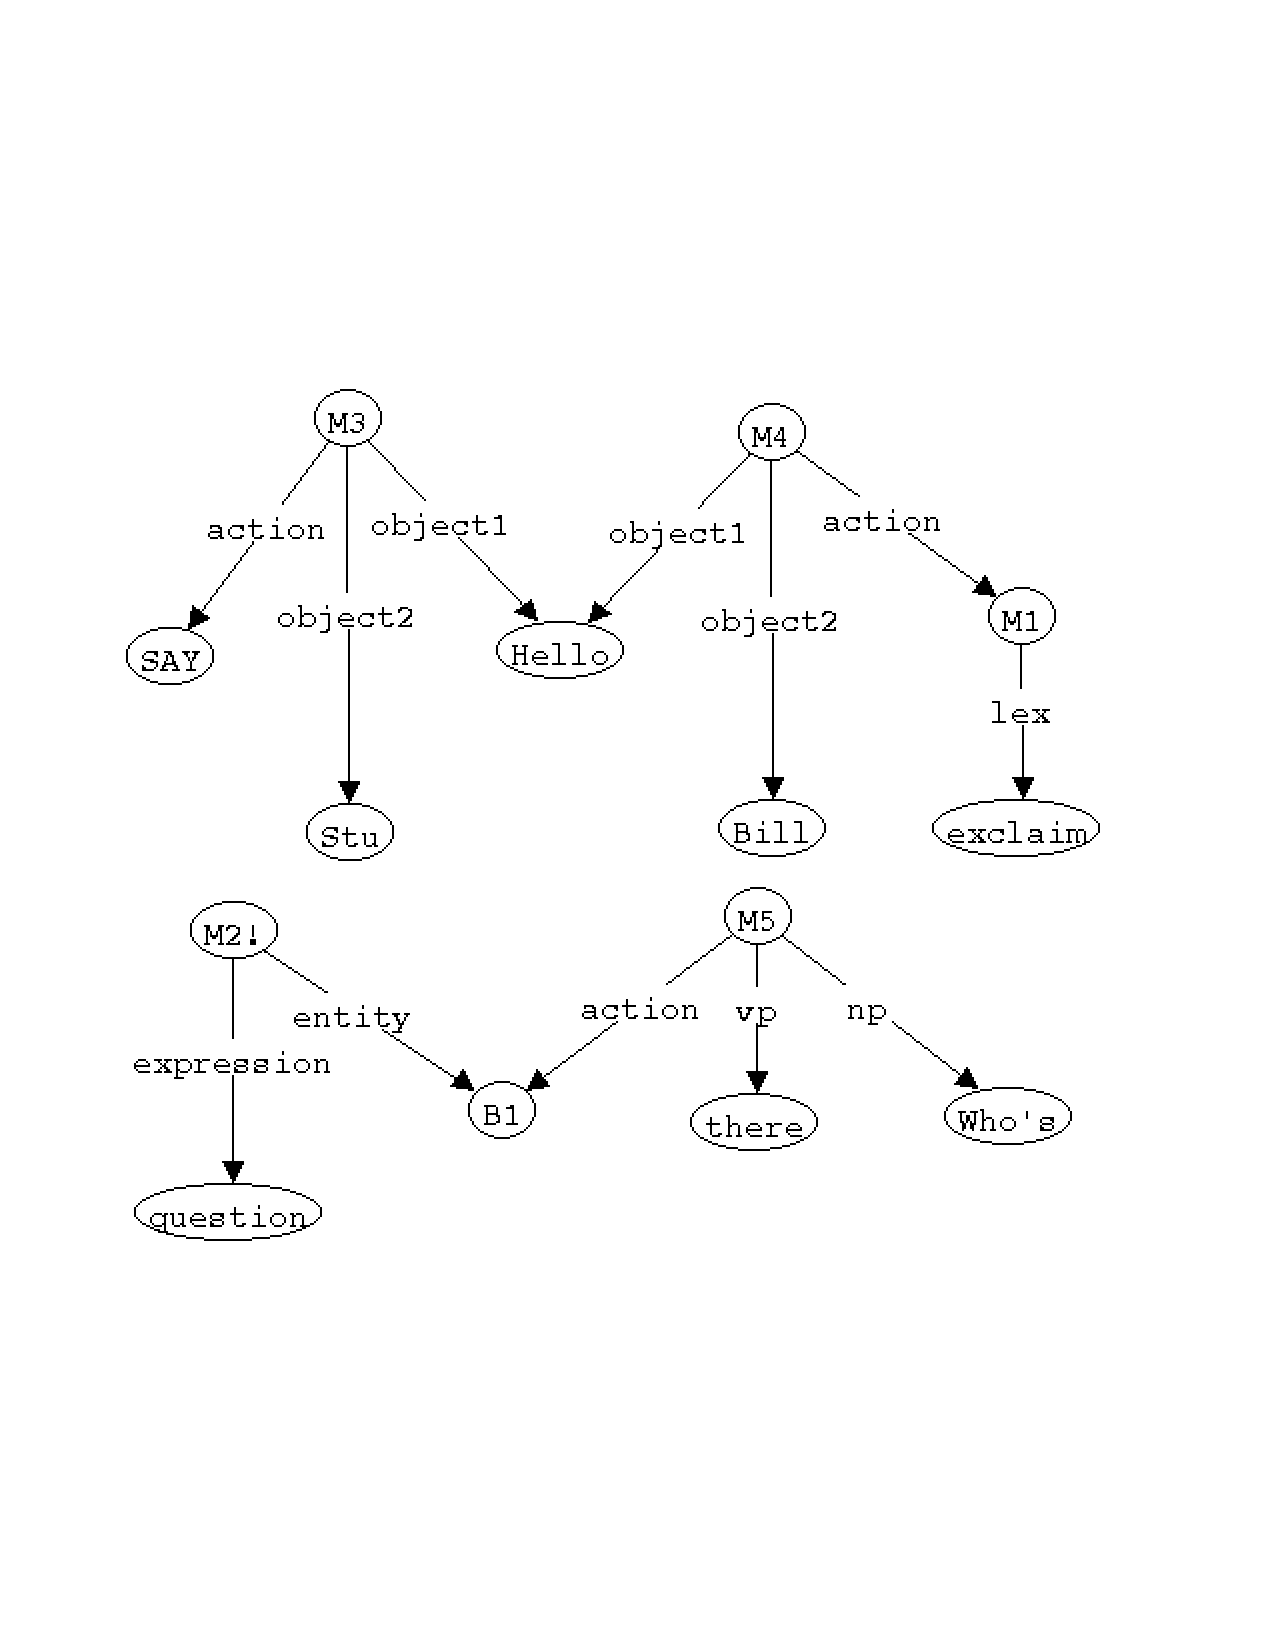
\includegraphics{snerefig1.pdf}}
\caption{Three ways of associating action nodes with action
functions. \ct{M3}, \ct{M4}, and \ct{M5} are act nodes, with action
nodes \ct{SAY}, \ct{M1}, and \ct{B1} respectively.}\label{snerefig1}
\end{figure}
The \ct{attach-primaction} call shown above associated action node \ct{SAY}
with the primitive action function \ct{sayfun}, action node \ct{M1}
with the primitive action function \ct{exclaimfun}, and action node
\ct{B1} with the primitive action function \ct{questionfun}.

The user must remember to use \ct{attach-primaction} to associate
action nodes even with the built-in primitive action functions she
intends to use.  As a reminder, the built in action functions are
listed in Table~\ref{primftable}.  The \ct{achieve} primitive action
function will be described below.
\begin{table}[htb]
\caption{Built-in Primitive Action
Functions}\label{primftable}\index{primitive action functions!table of}
\begin{center}\ttfamily
\begin{tabular}{llll}
believe & disbelieve & adopt & unadopt\\
achieve & do-one & do-all & snsequence\\
snif & sniterate & withsome & withall
\end{tabular}
\end{center}
\end{table}

\section{Defined Acts}
An act that is not a primitive act is called a {\em defined act.}  If
SNeRE is asked to perform a defined act, it will try to infer a {\em
plan} to carry out the act.  A {\em plan} in the SNeRE formalism is
represented by any act node, but especially one whose action is a
control action.  A node of the form {\ttfamily M:\{$\langle$plan, p$\rangle,
\langle$act, a$\rangle$\}}\indexct{plan-act}\indexct{act-plan}, where
\ct{a} is a defined act node, and \ct{p} is a plan node, represents the
proposition that the plan represented by \ct{p} is the way to perform
the defined act represented by \ct{a}.  Having inferred some plans for
carrying out a defined act, SNeRE will perform \ct{do-one} on them.

\pagebreak
To illustrate the use of defined acts, we will first define \ct{say}
as a one object action function, and associate action nodes with the
functions \ct{say}, and \ct{snsequence}.
\begin{verbatim}
^^
--> (define-primaction say (object1)
      "Print the object."
      (format t "~&~A" (sneps:choose.ns object1)))
SAY
--> (attach-primaction
      say say
      snsequence snsequence)
T
--> ^^
 CPU time : 0.05 
\end{verbatim}
Then, we will give a rule that says the way to greet a person is to
\ct{sayHi}, then say the person's name (and assert that Stu and Bill
are people).
\begin{verbatim}
* (describe (assert forall $person
                    ant    (build member *person class person)
                     cq    (build act  (build action greet object1 *person)
                                  plan (build action  snsequence
                                              object1 sayHi
                                              object2 (build action  say
                                                             object1 *person)))))

(M1! (FORALL V1) (ANT (P1 (CLASS PERSON) (MEMBER V1)))
 (CQ
  (P5 (ACT (P2 (ACTION GREET) (OBJECT1 V1)))
   (PLAN
    (P4 (ACTION SNSEQUENCE) (OBJECT1 SAYHI)
     (OBJECT2 (P3 (ACTION SAY) (OBJECT1 V1))))))))
(M1!)
 CPU time : 0.18 

* (describe (assert member (Stu Bill) class person))
(M2! (CLASS PERSON) (MEMBER BILL STU))
(M2!)
 CPU time : 0.06 

\end{verbatim}
We will give three plans for \ct{sayHi}.
\begin{verbatim}
* (describe (assert act  sayHi
                    plan (build action say object1 "Hello")))
(M4! (ACT SAYHI) (PLAN (M3 (ACTION SAY) (OBJECT1 Hello))))
(M4!)
 CPU time : 0.09 

* (describe (assert act  sayHi
                    plan (build action say object1 "Hi")))
(M6! (ACT SAYHI) (PLAN (M5 (ACTION SAY) (OBJECT1 Hi))))
(M6!)
 CPU time : 0.06 
\end{verbatim}
\pagebreak
\begin{verbatim}
* (describe (assert act  sayHi
                    plan (build action say object1 "Hiya")))
(M8! (ACT SAYHI) (PLAN (M7 (ACTION SAY) (OBJECT1 Hiya))))
(M8!)
 CPU time : 0.09 
\end{verbatim}
and finally, \ct{greet} Stu and Bill.
\begin{verbatim}
* (perform (build action greet object1 Stu))
Hiya
STU
 CPU time : 1.34 

* (perform (build action greet object1 Bill))
Hello
BILL
 CPU time : 1.37 
\end{verbatim}
A defined act node may be represented by a node with no \ct{action}
arc emanating from it, as long as a plan can be derived for it.
\begin{verbatim}
* (describe (assert act  ask
                    plan (build action say object1 "Who's there?")))
(M7! (ACT ASK) (PLAN (M6 (ACTION SAY) (OBJECT1 Who's there?))))
(M7!)
 CPU time : 0.05 

* (perform ask)
Who's there?
 CPU time : 0.33 
\end{verbatim}

\section{Goals}
In the SNeRE formalism, a {\em goal} is a proposition that the SNeRE
agent is trying to bring about.  The action of trying to bring about a
goal is called ``\ct{achieve}'':
\begin{description}
\item[{\ttfamily(achieve {\itshape object1})},]\indexct{achieve} where
\cv{object1} must be a proposition node, is performed by finding plans for
achieving \cv{object1}, and performing a \ct{do-one} on them.
\end{description}

The plans for achieving goals are given by assertions of the form {\ttfamily
M!:\{$\langle$goal, g$\rangle, \langle$plan,
p$\rangle$\}},\indexct{goal-plan}\indexct{plan-goal} which says that
\ct{p} is a plan for achieving the goal \ct{g}.
\begin{verbatim}
* (describe
   (assert forall $person
           ant    (build member *person class person)
            cq    (build goal (build agent *person state is location here)
                         plan (build action call object1 *person))))
(M22! (FORALL V5) (ANT (P23 (CLASS PERSON) (MEMBER V5)))
 (CQ
  (P26 (GOAL (P24 (AGENT V5) (LOCATION HERE) (STATE IS)))
   (PLAN (P25 (ACTION CALL) (OBJECT1 V5))))))
(M22!)
 CPU time : 0.18 

* (describe (assert forall $person
                    ant    (build member *person class person)
                     cq    (build act  (build action call object1 *person)
                                  plan (build action  snsequence
                                              object1 (build action  say
                                                             object1 "Come here")
                                              object2 (build action  say
                                                             object1 *person)))))
(M24! (FORALL V6) (ANT (P27 (CLASS PERSON) (MEMBER V6)))
 (CQ
  (P31 (ACT (P28 (ACTION CALL) (OBJECT1 V6)))
   (PLAN
    (P30 (ACTION SNSEQUENCE) (OBJECT1 (M23 (ACTION SAY) (OBJECT1 Come here)))
     (OBJECT2 (P29 (ACTION SAY) (OBJECT1 V6))))))))
(M24!)
 CPU time : 0.19 

* (perform (build action  achieve
                  object1 (build agent Bill state is location here)))
Come here
BILL
 CPU time : 1.76 
\end{verbatim}

\section{The Execution Cycle: Preconditions and Effects}\label{executive:sec}
SNeRE acting may be understood by the following pseudo-definition of
\ct{perform}, although the actual implemention is different.
\indexct{perform}
\begin{tabbing}
\ttfamily per\=\ttfamily form(act):\\
\>\ttfamily preconds := {\itshape set of preconditions of} act;\\
\>\ttfamily unachieved-preconditions := preconds - \{p | p $\in$ precond \&
p {\itshape is deduceable}\};\\
\>\ttfamily if \=\ttfamily unachieved-preconditions $\neq$ nil\\
\>\>\ttfamily then perform(snsequence(\=\ttfamily doall(\{a | p $\in$
unachieved-preconditions \& a = achieve(p)\}),\\
\>\>\>\ttfamily act))\\
\>\>\ttfamily else \{\=\ttfamily effects := {\itshape effects of} act;\\
\>\>\>\ttfamily if \=\ttfamily act {\itshape is primitive}\\
\>\>\>\>\ttfamily then \{\=\ttfamily apply(primitive-function(act), objects(act));\\
\>\>\>\>\>\ttfamily doall(\{a | p $\in$ effects \& a = believe(p)\})\}\\
\>\>\>\>\ttfamily else \{\=\ttfamily plans := {\itshape plans for carrying out} act;\\
\>\>\>\>\>\ttfamily perform(snsequence(\=\ttfamily do-one(plans),\\
\>\>\>\>\>\>\ttfamily doall(\{a | p $\in$ effects \& a = believe(p)\})))\}\}.
\end{tabbing}
Notes and comments:
\begin{itemize}
\item A trace of the acting system is printed when the global variable
\ct{*plantrace*}\indexglobal{plantrace} is set to \ct{T}.  If
\ct{*plantrace*} is set to \ct{'surface}, then nodes are sent to the
GATN generator starting at state \ct{G} for printing.  If
\ct{*plantrace*} is \ct{NIL}, no trace is printed.  This was the
setting for the previous examples in this chapter, but the default is
\ct{T}.

\item The preconditions of an act, \ct{a} are all \ct{p} for which
propositions of
the form {\ttfamily M!:\{$\langle$act, a$\rangle$, $\langle$precondition,
p$\rangle$\}}\indexct{act-precondition} are deduceable.
\begin{verbatim}
* (describe
     (assert forall *person
             ant    (build member *person class person)
              cq    (build act          (build action greet object1 *person)
                           precondition (build agent    *person
                                               state    is
                                               location here))))
(M34! (FORALL V6) (ANT (P27 (CLASS PERSON) (MEMBER V6)))
 (CQ
  (P40 (ACT (P39 (ACTION GREET) (OBJECT1 V6)))
   (PRECONDITION (P38 (AGENT V6) (LOCATION HERE) (STATE IS))))))
(M34!)
 CPU time : 0.13 

* (perform (build action greet object1 Stu))
About to do 
((M9 (ACTION (GREET)) (OBJECT1 (STU))))

I wonder if the act 
((M9 (ACTION (GREET)) (OBJECT1 (STU))))
has any preconditions...

The act 
((M9 (ACTION (GREET)) (OBJECT1 (STU))))
has a precondition:
((M35! (ACT (M9 (ACTION (GREET)) (OBJECT1 (STU))))
  (PRECONDITION (M33! (AGENT (STU)) (LOCATION (HERE)) (STATE (IS))))))
It is satisfied.

The act 
((M9 (ACTION (GREET)) (OBJECT1 (STU))))
has a plan:
((M12! (ACT (M9 (ACTION (GREET)) (OBJECT1 (STU))))
  (PLAN
   (M11 (ACTION (SNSEQUENCE)) (OBJECT1 (SAYHI))
    (OBJECT2 (M10 (ACTION (SAY)) (OBJECT1 (STU))))))))

Intending to do
((M14 (ACTION (DO-ONE))
  (OBJECT1
   (M11 (ACTION (SNSEQUENCE)) (OBJECT1 (SAYHI))
    (OBJECT2 (M10 (ACTION (SAY)) (OBJECT1 (STU))))))))

Now doing: DO-ONE 
((M11 (ACTION (SNSEQUENCE)) (OBJECT1 (SAYHI))
  (OBJECT2 (M10 (ACTION (SAY)) (OBJECT1 (STU))))))

Chose to do the act 
((M11 (ACTION (SNSEQUENCE)) (OBJECT1 (SAYHI))
  (OBJECT2 (M10 (ACTION (SAY)) (OBJECT1 (STU))))))

About to do 
((SAYHI))

I wonder if the act 
((SAYHI))
has any preconditions...

The act 
((SAYHI))
has no preconditions:

The act 
((SAYHI))
has the following plans:
((M4! (ACT (SAYHI)) (PLAN (M3 (ACTION (SAY)) (OBJECT1 (Hello)))))
 (M6! (ACT (SAYHI)) (PLAN (M5 (ACTION (SAY)) (OBJECT1 (Hi)))))
 (M8! (ACT (SAYHI)) (PLAN (M7 (ACTION (SAY)) (OBJECT1 (Hiya))))))

Intending to do
((M15 (ACTION (DO-ONE))
  (OBJECT1 (M3 (ACTION (SAY)) (OBJECT1 (Hello)))
   (M5 (ACTION (SAY)) (OBJECT1 (Hi))) (M7 (ACTION (SAY)) (OBJECT1 (Hiya))))))

Now doing: DO-ONE 
((M3 (ACTION (SAY)) (OBJECT1 (Hello)))
 (M5 (ACTION (SAY)) (OBJECT1 (Hi)))
 (M7 (ACTION (SAY)) (OBJECT1 (Hiya))))

Chose to do the act 
((M3 (ACTION (SAY)) (OBJECT1 (Hello))))

About to do 
((M3 (ACTION (SAY)) (OBJECT1 (Hello))))

I wonder if the act 
((M3 (ACTION (SAY)) (OBJECT1 (Hello))))
has any preconditions...

The act 
((M3 (ACTION (SAY)) (OBJECT1 (Hello))))
has no preconditions:

Hello

About to do 
((M10 (ACTION (SAY)) (OBJECT1 (STU))))

I wonder if the act 
((M10 (ACTION (SAY)) (OBJECT1 (STU))))
has any preconditions...

The act 
((M10 (ACTION (SAY)) (OBJECT1 (STU))))
has no preconditions:

STU
 CPU time : 3.10 
\end{verbatim}

\item The current version of SNeRE will never give up trying to
achieve the preconditions of an act it is trying to perform, even if
some precondition is impossible to achieve.

\item The effects of an act, \cv{a} are all \cv{e} for which propositions of
the form {\ttfamily M!:\{$\langle$act, \cv{a}$\rangle$, $\langle$effect,
\cv{e}$\rangle$\}}\indexct{act-effect} are deduceable.
\begin{verbatim}
* (describe
   (assert forall *person
           ant    (build member *person class person)
            cq    (build act    (build action call object1 *person)
                         effect (build agent    *person
                                       state    is
                                       location here))))

(M36! (FORALL V6) (ANT (P27 (CLASS PERSON) (MEMBER V6)))
 (CQ
  (P41 (ACT (P28 (ACTION CALL) (OBJECT1 V6)))
   (EFFECT (P38 (AGENT V6) (LOCATION HERE) (STATE IS))))))
(M36!)
 CPU time : 0.11 

* (perform (build action call object1 Bill))
About to do 
((M27 (ACTION (CALL)) (OBJECT1 (BILL))))

I wonder if the act 
((M27 (ACTION (CALL)) (OBJECT1 (BILL))))
has any preconditions...

The act 
((M27 (ACTION (CALL)) (OBJECT1 (BILL))))
has no preconditions:

The act 
((M27 (ACTION (CALL)) (OBJECT1 (BILL))))
has a plan:
((M31! (ACT (M27 (ACTION (CALL)) (OBJECT1 (BILL))))
  (PLAN
   (M30 (ACTION (SNSEQUENCE))
    (OBJECT1 (M23 (ACTION (SAY)) (OBJECT1 (Come here))))
    (OBJECT2 (M17 (ACTION (SAY)) (OBJECT1 (BILL))))))))
\end{verbatim}
\pagebreak
\begin{verbatim}
Intending to do
((M40 (ACTION (DO-ONE))
  (OBJECT1
   (M30 (ACTION (SNSEQUENCE))
    (OBJECT1 (M23 (ACTION (SAY)) (OBJECT1 (Come here))))
    (OBJECT2 (M17 (ACTION (SAY)) (OBJECT1 (BILL))))))))

Now doing: DO-ONE 
((M30 (ACTION (SNSEQUENCE))
  (OBJECT1 (M23 (ACTION (SAY)) (OBJECT1 (Come here))))
  (OBJECT2 (M17 (ACTION (SAY)) (OBJECT1 (BILL))))))

Chose to do the act 
((M30 (ACTION (SNSEQUENCE))
  (OBJECT1 (M23 (ACTION (SAY)) (OBJECT1 (Come here))))
  (OBJECT2 (M17 (ACTION (SAY)) (OBJECT1 (BILL))))))

About to do 
((M23 (ACTION (SAY)) (OBJECT1 (Come here))))

I wonder if the act 
((M23 (ACTION (SAY)) (OBJECT1 (Come here))))
has any preconditions...

The act 
((M23 (ACTION (SAY)) (OBJECT1 (Come here))))
has no preconditions:

Come here

About to do 
((M17 (ACTION (SAY)) (OBJECT1 (BILL))))

I wonder if the act 
((M17 (ACTION (SAY)) (OBJECT1 (BILL))))

has any preconditions...
The act 
((M17 (ACTION (SAY)) (OBJECT1 (BILL))))

has no preconditions:

BILL

Now doing: DO-ALL 
((M38 (ACTION (BELIEVE))
  (OBJECT1 (M25 (AGENT (BILL)) (LOCATION (HERE)) (STATE (IS))))))

Believe 
(M25! (AGENT BILL) (LOCATION HERE) (STATE IS))
 CPU time : 2.07 
\end{verbatim}

\item The current version of SNeRE will believe that all effects of an
act are achieved, even though this may be a naive assumption.

\item The current version of the primitive action function \ct{do-all}
is\indexct{do-all}
\begin{verbatim}
(define-primaction do-all (object1)
  (do.ns (act object1)
         (schedule-act act)))
\end{verbatim}
but the user could redefine it if she wanted to make a more
intelligent decision about the order in which the acts should be
performed.

\item The current version of the primitive action function \ct{do-one}
is\indexct{do-one}\label{doonedef}
\begin{verbatim}
(define-primaction do-one (object1)
  (schedule-act
   (lisp-list-to-ns (if snip::*choose-randomly*
                        (nth (random (cardinality.ns object1))
                             (ns-to-lisp-list object1))
                      (first (ns-to-lisp-list object1))))))
\end{verbatim}
but the user could redefine it if she wanted to make a more
intelligent decision about which act should be performed.
\end{itemize}

\chapter{Program Interface}\label{interfacechap}
\section{Transformers}
These functions convert Lisp objects to SNePS nodes, and vice versa.

\docfun{apply-function-to-ns}{{\it fn ns}}
Converts the node set {\it ns} to a list of lisp objects, applies the
function {\it fn} to that list, then converts the result to a node
set, and returns that.

\docfun{lisp-list-to-ns}{{\it list}}
Returns a set of nodes whose identifiers look like the printed
representations of the objects in the list {\it list.}

\docfun{ns-to-lisp-list}{{\it ns}}
Returns a list of Lisp objects corresponding to the SNePS nodes in
the node set {\it ns.}

\docfun{node-to-lisp-object}{{\it nde}}
Returns a Lisp object corresponding to the SNePS node {\it nde.}
The Lisp object will be either a number or a symbol.

\docfun{lisp-object-to-node}{{\it obj}}
Returns a SNePS node whose identifier looks like {\it obj.}

\section{With-SNePSUL Reader Macro}\label{withreadersect}
The with-snepsul reader macro is provided so that users can easily
incorporate calls to SNePSUL commands within Lisp code.

\vspace{3ex}\par\noindent\ct{(\#$[i]$! ({\it snepsul-form$_1 \ldots$ snepsul-form$_n$}))}\index{\#"!@\ct{\#"!}}
The form following {\tt \#$[i]$\@!} is taken to be a list of SNePSUL
forms, each of which will be executed just as if it had been typed that
way at the SNePS prompt, regardless of the package in which the {\tt
\#$[i]$!} form is read. References to Lisp variables can be made via a
\verb|~| reader macro mechanism (similar to the comma within backquote
syntax).  Results of \verb|~| expansions will be automatically interned into
the SNePSUL package (i.e., any symbols that might be part of such a
result), unless explicitly specified otherwise. All the special reader
syntax available at the SNePS top-level is available, too.

\pagebreak
The semantics of the \verb|~| syntax is:\\[2ex]
\verb|~| {\it s-expression}:\\
S-expression will be read with ordinary reader syntax and at execution
time it will be evaluated and its value inserted into the SNePSUL
expression. If the value is a symbol or a list containing symbols then
these symbols will be interned into the SNePSUL package first.\\  Ex:
{\tt \#!((describe \verb|~|'(m1 m2)))} will act like {\tt (describe (m1
m2))}.\\[2ex]
\verb|~@| {\it s-expression}:\\
Just like \verb|~| but the value of the s-expression has to be a list
which will be spliced into the SNePSUL expression. Any symbols
occuring as leaves in the list will be interned into the SNePSUL
package first.  Ex: {\tt \#!((describe \verb|~@|'(m1 m2)))} will act
like {\tt (describe m1 m2)}.\\[2ex]
\verb|~~| {\it s-expression}:\\
Just like \verb|~| but symbols in the value will not be interned
into the SNePSUL package.\\[2ex]
\verb|~~@| {\it s-expression}:\\
Just like \verb|~@| but symbols in the value will not be
interned into the SNePSUL package.

CAUTION: The \verb|~| syntax can only be used within SNePSUL forms, but
not to denote multiple forms, e.g., while \verb|#!(~com1 ~com2 ~com3)| is
legal (as long as the runtime values of {\tt com$_i$} represent proper
SNePSUL commands), \verb|#!(~@commands)| is not!!

Supplying an optional digit argument can be used to select a
specific evaluation function, or to suppress output:
\begin{center}
\begin{tabular}{clcl}
  arg   &    eval function &     silent &       syntax\\
no arg  &     topsneval    &       no   & \tt     \#!(....)\\
  1     &     topsneval    &       no   & \tt     \#1!(....)\\
  2     &     eval         &       no   & \tt     \#2!(....)\\
  3     &     topsneval    &       yes  & \tt     \#3!(....)\\
  4     &     eval         &       yes  & \tt     \#4!(....)
\end{tabular}
\end{center}
For example, {\tt \#4!((build relation node))} will use the function
{\tt eval} to evaluate the form (hence {\tt build} can be used!!), and
will suppress any output generated by the snepsul command.

\subsection{Controlling the Evaluation of SNePSUL Forms Generated by \#!}

{\tt(defvar *with-snepsul-eval-function* \#'with-snepsul-standard-eval\\
{\rmfamily ``The value of this variable has to be a function of two
arguments, an {\it eval-function} and a {\it form} to which the
function should be applied.  Binding this variable to different
functions can implement various different evaluation behaviors, such
as normal evaluation, tracing, top-level-like echoing, evaluating and
printing the result, etc., when the {\it form} gets evaluated inside
{\tt with-snepsul-eval}.''})}

The following evaluation functions are available:

\docfun{with-snepsul-standard-eval}{{\it function form}}
Standard function used by {\tt with-snepsul-eval} to evaluate {\it
form} with evaluation {\it function}.

\docfun{with-snepsul-trace-eval}{{\it function form}}
Does not actually evaluate {\it form}, only prints it for debugging purposes.

\docfun{with-snepsul-toplevel-style-eval}{{\it function form}}
Evaluates the SNePSUL {\it form} using {\it function} and returns the
result.  Additionally, prints the prompt, {\it form}, result and
timing information just like the top-level SNePS loop does---good for
monitoring the execution of the actual SNePSUL commands.

\subsection{Example Use of \#!}
\begin{verbatim}
> (in-package 'user)
#<Package "USER" 79D15E>

> (defun myassert (relation nodes)
    (let ((base-node-var 'mybase))
      #!((define ~relation ~~relation myrel snip::test)
         (assert ~relation (~@nodes) snip::test #~base-node-var)
         (describe ~@(setq nodes (cdr nodes)))
         (assert ~~relation (~~@nodes) myrel *~base-node-var)
         (assert arg (build myrel hans ~relation franz)
                 myrel *mybase)
         (describe *nodes))))
MYASSERT

;; If the variable *with-snepsul-eval-function* is bound to the
;; function #'with-snepsul-trace-eval then the generated SNePSUL
;; expression will only be printed, but not actually executed:

> (let ((sneps:*with-snepsul-eval-function*
          #'sneps:with-snepsul-trace-eval))
    (myassert 'relrel '(hans franz otto)))
(SNEPS:DEFINE SNEPSUL::RELREL ;; Note "snepsulization" with single ~
              USER::RELREL    ;; Package preservation with double ~
              SNEPSUL::MYREL  ;; Unqualified symbols go into SNePSUL
              SNIP::TEST)     ;; Qualified symbols keep their package
(SNEPS:ASSERT SNEPSUL::RELREL
              (SNEPSUL::HANS SNEPSUL::FRANZ
                             SNEPSUL::OTTO)
              SNIP::TEST
              ;; had to replace the |'s with !'s here (comment problem)
              (SNEPS:!#! 'SNEPSUL::MYBASE))    ;; Combination of # and ~
(SNEPS::DESCRIBE SNEPSUL::FRANZ SNEPSUL::OTTO)
(SNEPS:ASSERT USER::RELREL (USER::FRANZ USER::OTTO)
              SNEPSUL::MYREL (SNEPS:* 'SNEPSUL::MYBASE))
(SNEPS:ASSERT SNEPS:ARG (SNEPS:BUILD SNEPSUL::MYREL SNEPSUL::HANS
                                     SNEPSUL::RELREL SNEPSUL::FRANZ)
              SNEPSUL::MYREL (SNEPS:* 'SNEPSUL::MYBASE))
(SNEPS::DESCRIBE (SNEPS:* 'SNEPS:NODES))

;; Now actually run it:
> (myassert 'relrel '(hans franz otto))
(FRANZ)
(OTTO)

(B1)
(FRANZ)    ;; user::franz
(FRANZ)    ;; snepsul::franz
(HANS)
(M1! (RELREL FRANZ HANS OTTO))
(M2! (RELREL FRANZ OTTO))
(M3 (MYREL HANS) (RELREL FRANZ))
(M4! (ARG (M3)))
(M5! (RELREL FRANZ HANS OTTO)
     (TEST B1))
(M6! (MYREL B1)
     (RELREL FRANZ OTTO))
(M7! (ARG (M3)) (MYREL B1))
(B1 FRANZ FRANZ HANS M1! M2! M3 M4! M5! M6! M7! OTTO OTTO)
SNEPS:DEFAULT-DEFAULTCT

;; Here's what the definition of myassert looks like:
> (ppdef 'myassert)
(LAMBDA (RELATION NODES)
  (BLOCK MYASSERT
    (LET ((BASE-NODE-VAR 'MYBASE))
      (PROGN ;; progn generated by #!
        (SNEPS::WITH-SNEPSUL-EVAL
            `(SNEPS:DEFINE ,(SNEPS::SNEPSULIZE RELATION) ,RELATION
              SNEPSUL::MYREL SNIP::TEST)
          #'SNEPS:TOPSNEVAL NIL)
        (SNEPS::WITH-SNEPSUL-EVAL
            `(SNEPS:ASSERT ,(SNEPS::SNEPSULIZE RELATION)
              (,@(SNEPS::SNEPSULIZE NODES)) SNIP::TEST
              (SNEPS:!#! ',(SNEPS::SNEPSULIZE BASE-NODE-VAR)))
          #'SNEPS:TOPSNEVAL NIL)
        (SNEPS::WITH-SNEPSUL-EVAL
            `(SNEPS::DESCRIBE
              ,@(SNEPS::SNEPSULIZE (SETQ NODES (CDR NODES))))
          #'SNEPS:TOPSNEVAL NIL)
        (SNEPS::WITH-SNEPSUL-EVAL
            `(SNEPS:ASSERT ,RELATION (,@NODES) SNEPSUL::MYREL
              (SNEPS:* ',(SNEPS::SNEPSULIZE BASE-NODE-VAR)))
          #'SNEPS:TOPSNEVAL NIL)
        (SNEPS::WITH-SNEPSUL-EVAL
            `(SNEPS:ASSERT SNEPS:ARG
              (SNEPS:BUILD SNEPSUL::MYREL SNEPSUL::HANS
               ,(SNEPS::SNEPSULIZE RELATION) SNEPSUL::FRANZ)
              SNEPSUL::MYREL (SNEPS:* 'SNEPSUL::MYBASE))
          #'SNEPS:TOPSNEVAL NIL)
        (SNEPS::WITH-SNEPSUL-EVAL
            '(SNEPS::DESCRIBE (SNEPS:* 'SNEPS:NODES))
          #'SNEPS:TOPSNEVAL NIL)))))
\end{verbatim}
\pagebreak
\section{Defining New Commands}

\docfun{defsnepscom}{{\it command} ([(\{{\it arg}\}$^*$)] [{\it
environments}] [{\it eval-args}]) \{{\it body-form}\}$^*$}

{\tt defsnepscom} is a Lisp macro that defines SNePSUL commands. All
standard SNePSUL commands such as \ct{find}, \ct{assert}, \ct{deduce},
etc., are defined via \ct{defsnepscom}. More importantly, \ct{defsnepscom}
is the only way to define commands which will be recognized as legal
SNePSUL commands at the SNePS top level. The syntax of \ct{defsnepscom}
is very similar to that of a standard \ct{defun} or \ct{defmacro}.

{\it command} is a Lisp symbol which serves as the command name, e.g.,
\ct{find}, \ct{deduce}, \ct{my-find}, \ct{isa}, etc. {\it command}
will get exported automatically from its home package and imported
into the SNePSUL package, hence, even if the command was defined in a
different package, it can be used at the SNePS top level without
package qualifiers. The only catch is that if {\it command} is the
name of a standard {\sc Common Lisp} function as in the case of \ct{find} or
\ct{assert}, then that symbol has to be shadowed in its home package with
the {\sc Common Lisp} function \ct{shadow} before the command gets
defined.

\ct{(\{{\it arg}\}$^*$)} is an optional argument list in the standard
{\sc Common Lisp} syntax.  An actual call to the command has to be
legal according to that argument list, otherwise an error will
occur. The only difference to the standard \ct{defun} style of
specifying argument lists is an extra level of nesting as shown in the
examples below.

The optional second argument {\it environments} defines the places in
which the command can legally appear. An environment is basically a
specification of a location in which a command can be used. For
example, some commands can only be used at the top level, some
commands can never be used at the top level but only inside some other
command, some commands can only be used within \ct{find} commands,
etc. See Section~\ref{environsect} for more information on
environments.  {\it environments} can either be \ct{:all} to define
{\it command} as legal in all possible environments, or it can be a
subset of \ct{(top rs bns fns ons rearrange)} specified as a
list, which will make it legal in the specified environments.  These
abbreviations indicate environments as specified in the following
table.
\begin{center}
\begin{tabular}{ll}
\tt top & The top level of SNePS~2\\
\tt rs & A {\em relation-set} position embedded in a command\\
\tt bns & A {\em node-set} position in {\tt build}\\
\tt fns & A {\em node-set} position in {\tt find} or {\tt findassert}\\
\tt ons & A {\em node-set} position in any of the other commands\\
\tt rearrange & The command is an infix or postfix command.
\end{tabular}
\end{center}
A third possibility, which is probably
the one most commonly used, is to supply the name of an already
existing command, in which case {\it command} will be legal in all
environments in which the supplied command is legal. {\it
environments} defaults to \ct{(top)}. According to the specified {\it
environments}, \ct{defsnepscom} automatically updates the SNePSUL
variables \ct{commands}, \ct{topcommands}, etc. (See
Section~\ref{variablessect}.)

By default, commands defined with \ct{defsnepscom} do not evaluate their
arguments. If one wants command arguments to be evaluated before they get
passed (similar to the behavior of standard functions defined with \ct{defun}),
one has to specify the optional third argument, {\it eval-args} as \ct{t}.

{\it body-form\/}s are a sequence of body forms, possibly including a
documentation string and declarations just as in a normal \ct{defun}. The
value/s of the last form will be returned.

Here are some examples:

\subsection*{Example 1:}
\begin{verbatim}
* ^^   ;; escape to the Lisp level, since `defnepscom' is not a SNePSUL command

--> (defsnepscom mylist ((first &optional second &rest others))
       (list first second others))
T
--> ^^ ;; back to the SNePS top level

 CPU time : 0.03 

* (mylist apples oranges hans franz)  ;; let's try it out:

(APPLES ORANGES (HANS FRANZ))

 CPU time : 0.01
\end{verbatim}
Note, that we did not have to quote \ct{apples} and \ct{oranges} in
the example above, because {\it eval-args} was not specified as \ct{t}.

\subsection*{Example 2:}
\begin{verbatim}
* ^^

--> (defsnepscom isa ((who what) assert)
      "Asserts that WHO is a WHAT."
      #!((assert member ~who class ~what)))
T
--> ^^

 CPU time : 0.08 

* (describe (isa hans student))

(M1! (CLASS STUDENT) (MEMBER HANS))

(M1!)

 CPU time : 0.02
\end{verbatim}
The \ct{isa} command defined above takes two arguments \ct{who} and
\ct{what}, and it is legal in all places where the \ct{assert} command
is legal, because we specified \ct{assert} as the value of {\it
environments}. The body of the command has a documentation string just
as a normal \ct{defun}, and it uses the \verb|#!| with-snepsul reader
macro (see Section~\ref{withreadersect}) to easily call the SNePSUL
command \ct{assert} in the body of the command definition.

\subsection*{Example 3:}
\begin{verbatim}
* ^^

--> (defsnepscom lex-build ((word) (top bns) t)
      "Builds a node with a `lex' arc to a WORD node."
      #2!((build lex ~word)))
T
--> ^^

 CPU time : 0.25 
\end{verbatim}
\pagebreak
\begin{verbatim}
* (lex-build (progn (format t "Word: ") (read)))
Word: Lucy

(M1)

 CPU time : 0.03 
\end{verbatim}
This last example command uses all the features: It has an argument list, it
explicitly specifies two environments in which the command will be legal, and
it evaluates its arguments which is the reason why we could call it with the
little interactive input specification. Note, that this command
\ct{build}s (not \ct{assert}s) a node, and that it will be available
as a top-level command because we specified \ct{top} as one of the
environments. For good reasons, the standard \ct{build} command is not a
top-level command, hence, in this example we forced SNePS to do
something which is normally not allowed.

By convention, every command that returns a node set should return a
context as a second value which will be used to display the node
set. Commands which use an application of the \verb|#!| reader macro
as their last body form will achieve this automatically. Otherwise, a
form such as \ct{(values nodes crntct)} has to be used as the last body
form.

\ct{defsnepscom} is available in all standard SNePS packages.  Hence, it can
normally always be used without a package qualifier. If it is used in
a non-standard package it should be written as \ct{sneps:defsnepscom}.


\docfun{undefsnepscoms}{ \{{\it commands}\}$^*$}
Undefines all {\it command\/}s. The function definitions of the
individual commands will not be removed, but the listed commands will
not be available as SNePSUL commands anymore. For example, the
following will undo the inappropriate definition of Example 3 above:
\begin{verbatim}
* (^ (undefsnepscoms lex-build))

(T)

 CPU time : 0.00 

* (lex-build Lucy)

SNePS ERROR: Invalid top SNePSUL form: (LEX-BUILD LUCY)
Occurred in module TOP-EVALUATOR in function TOPSNEVAL

Do you want to debug it? n

*
\end{verbatim}

\chapter{SNePSLOG}\label{snepslogchap}

\section{SNePSLOG Basics}
SNePSLOG is a logic programming interface to SNePS.  That is, almost
everything that can be done interactively using SNePSUL can be done
interactively using SNePSLOG, just with a syntax that looks more like
traditional symbolic logic than SNePSUL does.  Use of SNePSLOG rather
than SNePSUL is recommended for the SNePS novice.

To enter SNePSLOG, load SNePS and evaluate
\begin{center}
{\tt (snepslog)}
\end{center}
To leave SNePSLOG, execute the SNePSLOG command
\begin{center}
{\tt lisp}
\end{center}

The default Common Lisp package for symbols read by the SNePSLOG
reader is \texttt{snepslog}.

The full details of the SNePSLOG syntax is in \S\ref{sec:snepslogsyn}.  The
semantics are given in \S\ref{sec:snepslogsem}.

\section{SNePSLOG Syntax}\label{sec:snepslogsyn}
\newcommand{\oparen}{\texttt{\underline{(}}}
\newcommand{\cparen}{\texttt{\underline{)}}} 

The SNePSLOG syntax is described in Tables~\ref{tab:syntaxb} and
\ref{tab:syntaxa} using the Extended BNF notation.  
\begin{table}[hbp]
  \centering
  \caption{The Syntax of SNePSLOG Commands}
  \label{tab:syntaxb}
\begin{tabular}{|lcl|}\hline
command  &::=& wffNameCommand \verb.|. snepslogCommand \verb.|. wffCommand\\
wffNameCommand   &::=& wffName terminalPunctuation\\
wffCommand       &::=& wff terminalPunctuation \textit{; wff must not
  be an atomic symbol}\\
snepslogCommand &::=& \texttt{\%} \textit{SNePSULcommand}
                      \verb.|. \verb.^. \textit{LispForm} \verb.|. \verb.^^. \\
                 && \verb.|. \texttt{activate} wff [.]\\
                 && \verb.|. \texttt{activate!} wff [terminalPunctuation]\\
                 && \verb.|. \texttt{add-to-context} SNePSLOGsymbol termSet [.]\\
                 && \verb.|. \texttt{ask} wff [terminalPunctuation]\\
                 && \verb.|. \texttt{askifnot} wff [terminalPunctuation]\\
                 && \verb.|. \texttt{askwh} wff [terminalPunctuation]\\
                 && \verb.|. \texttt{askwhnot} wff [terminalPunctuation]\\
                 && \verb.|. \texttt{beliefs-about} pTermSet [.]\\
                 && \verb.|. \texttt{br-mode} [\texttt{auto}
                 \verb.|. \texttt{manual}] [.]\\
                 && \verb.|. \texttt{br-tie-mode} [\texttt{auto}
                 \verb.|. \texttt{manual}] [.]\\
                 && \verb.|. \texttt{clear-infer} [.]\\
                 && \verb.|. \texttt{clearkb} [.]\\
                 && \verb.|. \texttt{copyright} [.]\\
                 && \verb.|. \texttt{define-frame} SNePSLOGsymbol
                                \textit{LispList} [\textit{LispString}] [.]\\
                 && \verb.|. \texttt{define-path} \textit{SNePSRelation SNePSPath} [.]\\
                && \verb.|. \texttt{demo} [\textit{filePath}
                            \verb.|. \texttt{?} \verb.|. $i$]
                            [\verb.t | b | bv | a | av | n.] [.]\\
                && \verb.|. \texttt{describe-context} [SNePSLOGsymbol] [.]\\
                && \verb.|. \texttt{describe-terms} [pTermSet] [.]\\
                && \verb.|. \texttt{expert} [.]\\
                && \verb.|. \texttt{lisp} [.]\\
                && \verb.|. \texttt{list-asserted-wffs} [SNePSLOGsymbol] [.]\\
                && \verb.|. \texttt{list-contexts} [.]\\
                && \verb.|. \texttt{list-terms} [pTermSet] [.]\\
                && \verb.|. \texttt{list-wffs} [.]\\
                && \verb.|. \texttt{load} \textit{filePath} [.]\\
                && \verb.|. \texttt{normal} [.]\\
                && \verb.|. \texttt{perform} atomicTerm [.]\\
                && \verb.|. \texttt{remove-from-context} SNePSLOGsymbol pTermSet\\
                && \verb.|. \texttt{set-context} SNePSLOGsymbol [pTermSet]\\
                && \verb.|. \texttt{set-default-context} SNePSLOGsymbol \\
                && \verb.|. \texttt{set-mode-1}  [.]\\
                && \verb.|. \texttt{set-mode-2}  [.]\\
                && \verb.|. \texttt{set-mode-3} [\verb.t | nil.]  [.]\\
                && \verb.|. \texttt{set-order} (\texttt{explicit}
                \verb.|. \texttt{fluent} \verb.|. 
                \texttt{null-order} \verb.|. \texttt{source}
                \verb.|. \textit{LispSymbol})\\
                && \verb.|. \texttt{show} [pTermSet] [.]\\
                && \verb.|. \texttt{trace} [SNePSLOGfunction]* [.]\\
                && \verb.|. \texttt{undefine-path} \textit{SNePSRelation} [.]\\
                && \verb.|. \texttt{unlabeled} [.]\\
                && \verb.|. \texttt{untrace} [SNePSLOGfunction]* [.]\\
SNePSLOGfunction &::=& \verb.inference | acting | translation | parsing.\\
                && \verb.|. \textit{LispSymbol}\\\hline
\end{tabular}
\end{table}
\begin{table}[hbp]
  \centering
  \caption{The Syntax of SNePSLOG Wffs}
  \label{tab:syntaxa}
\begin{tabular}{|lcl|}\hline
wff              &::=& infixedTerm \verb.|. entailment \verb.|. prefixedTerm\\
infixedTerm      &::=& prefixedTerm [( \verb.and | or | <=>. ) prefixedTerm]+\\
entailment       &::=& termSet 
                       (\verb.=> | v=> | &=> |. \texttt{$i$=>})
                        termSet\\ 
pTermSet         &::=& termSet ; but taken to denote all terms that match\\
termSet          &::=& prefixedTerm \verb.| {. termSequence \verb.}.\\
termSequence     &::=& prefixedTerm [\texttt{,} prefixedTerm]*\\
prefixedTerm     &::=& negatedTerm \verb.|. andorTerm \verb.|. setTerm
                       \verb.|. threshTerm\\
                 &&  \verb.|. allTerm \verb.|. nexistsTerm \verb.|. atomicTerm\\
negatedTerm      &::=& \verb.~. atomicTerm\\
andorTerm        &::=& \texttt{andor} $\not\mathrm{b}$ \texttt{\oparen}$i$\texttt{,} $j$\cparen termSet 
                       $\mathit{; 0 <= i <= j}$\\ 
setTerm          &::=& (\texttt{and} \verb.|. \texttt{or} \verb.|.
     \texttt{nand} \verb.|. \texttt{nor} \verb.|. \texttt{xor} \verb.|.
     \texttt{iff}) $\not\mathrm{b}$ termSet\\
threshTerm       &::=& \texttt{thresh} $\not\mathrm{b}$ \oparen$i$ [\texttt{,} $j$]\cparen
                       termSet
                       $\mathit{; 0 <= i <= j}$\\
allTerm          &::=& \texttt{all \underline{(}} symbolSequence
                       \texttt{\underline{)}
                       \underline{(}} wff \texttt{\underline{)}}
                       \textit{; wff must not be an atomic symbol}\\ 
nexistsTerm      &::=& \texttt{nexists} $\not\mathrm{b}$ nexistsParameters
                     \oparen symbolSequence \cparen~
                     \oparen termSet \texttt{:} termSet \cparen\\
nexistsParameters &::=& \oparen $i$ \texttt{,} $j$ \texttt{,} $k$ \cparen
                     \verb.|. \oparen ~\texttt{\underline{~}} \texttt{,} $j$
                     \texttt{, \underline{~}}  \cparen
                     \verb.|. \oparen $i$ \texttt{, \underline{~}}
                     \texttt{,} $k$ \cparen\\ 
atomicTerm       &::=& wffName \verb.|. qvar \verb.|. SNePSLOGsymbol\\
                 &&    \verb.|.withsome/allTerm \textit{; in Mode 3 only}\\
                 &&    \verb.|. (qvar \verb.|. SNePSLOGsymbol)
                       \oparen termSetSequence \cparen\\
                 &&    \verb.|.\underline{(} wff \underline{)}\\
withsome/allTerm &::=& (withsome \verb.|. withall) \oparen
                       symbolSequence\texttt{,} termSet\texttt{,}
                       termSet [\texttt{,} ~termSet] \cparen\\
termSetSequence  &::=& termSet [\texttt{,} ~termSet]*\\
symbolSequence &::=& SNePSLOGsymbol [\texttt{,} SNePSLOGsymbol]*\\
wffName          &::=& \texttt{wff$i$} [!]
                       \textit{;} \texttt{wff$i$} \textit{must already
                         name a wff.}\\
qvar             &::=& \texttt{?} SNePSLOGsymbol\\
SNePSLOGsymbol   &::=& \texttt{wff$i$} \verb.|. \textit{Lispsymbol}
\verb.|. \textit{Lispstring} \verb.|. \textit{Lispnumber}\\
terminalPunctuation &::=& \texttt{.} \verb.|. \texttt{!}
                          \verb.|. \texttt{??}
                          \verb.|. \texttt{?} [~\oparen ~i~ [j]~ \cparen~]\\\hline
\end{tabular}
\end{table}
Object language terminal symbols are in \texttt{this font}. Grouping parentheses
are ( and ).  Alternatives are separated by the \verb.|.  character.  Square
brackets [ and ] surround optional material.  The Kleene star, *, indicates zero
or more repetitions.  The Kleene plus, +, indicates one or more repetitions.
The character ``$\mathrm{\not b}$'' indicates that whitespace is not allowed at
that position. Object language parentheses are \oparen~ and \cparen. The object
language comma is \texttt{,}.  The object language underscore character is
\texttt{\underline{~}}.  The symbols $i$, $j$, and $k$ are non-terminal symbols
representing integers.  Material starting with a semicolon is a comment
indicating a restriction on the syntax.

A SNePSLOG command may continue on subsequent lines as long as the SNePSLOG
command couldn't, according to the grammar, terminate on the initial line.  If
it could, and you want to continue the command on a subsequent line, end the
line with the character ``\verb.\.'' (without the quotation marks).

Note that a SNePSLOGsymbol may be any Lisp symbol, string, or number.
If a SNePSLOGsymbol is a symbol, it is interned in the
\texttt{snepslog} package.  If a SNePSLOGsymbol is a string, it is
coerced into a symbol whose symbol-name is the original string, and is
interned in the \texttt{snepslog} package.  If a SNePSLOGsymbol is a
number, it is coerced into a symbol whose symbol-name is the Lisp
printer representation of the original number, and is interned in the
\texttt{snepslog} package.  Two SNePSLOGsymbols are considered the
same by SNePSLOG if and only if the Lisp being used considers the
symbols constructed by this algorithm to be the same.  When SNePSLOG
prints a SNePSLOGsymbol, it does not print string-quotes nor escape
characters.

\section{SNePSLOG Semantics}\label{sec:snepslogsem}
\subsection{Semantics of SNePSLOG Commands}\label{snepslogcommands}
 
Here we present a list of the SNePSLOG commands,
with a description of what they do.  See Table~\ref{tab:syntaxb} for a
concise list of the SNePSLOG commands and their syntax.
\begin{itemize}
\item
\texttt{\%} \textit{SNePSULcommand}\indexct{\%} \\
Executes the \textit{SNePSULcommand}, and prints the result.  The
default Common Lisp package for symbols in the \textit{SNePSULcommand}
is \texttt{snepsul}.

\item
\verb|^| \textit{LispForm}\index{\_\_@\ct{\^{~}}} \\
Evaluates the \textit{LispForm}, and prints the result.

\item
\verb|^^|\index{\_\_\_@\ct{\^{~}\^{~}}} \\
Enters a Lisp read-eval-print loop. To leave the loop,
type {\tt end} or \verb|^^|.

\item \texttt{activate} wff\indexct{activate}\\
Performs forward inference on all asserted propositions that dominate the
wff.
  
\item \texttt{activate!} wff\index{activate"!@\ct{activate"!}}\\
  Asserts wff, and performs forward inference on it,
  and on all asserted propositions that dominate it.
  
\item\texttt{add-to-context} SNePSLOGsymbol termSet\indexct{add-to-context} \\
  Adds the wffs in termSet as hypotheses in the context named
  SNePSLOGsymbol.

\item \texttt{ask} wff\indexct{ask}\\
  Performs backward inference on wff and prints the inferred positive
  instances of it.
  
\item \texttt{askifnot} wff\indexct{askifnot}\\
  Performs backward inference on wff, and prints the
  inferred negative instances of it.
  
\item \texttt{askwh} wff\indexct{askwh}\\
  Performs backward inference on wff, and prints a list of
  substitutions, which, when applied to wff yield asserted wffs.
  
\item \texttt{askwhnot} wff\indexct{askwhnot}\\
  Performs backward inference on wff, and prints a list of
  substitutions, which, when applied to the negation of wff yield
  asserted wffs.
  
\item \texttt{beliefs-about} pTermSet\indexct{beliefs-about}\\
Returns a set of all the asserted wffs that dominate
the terms described by pTermSet.

\item \texttt{br-mode} [\texttt{auto}
  \verb.|. \texttt{manual}]\indexct{br-mode}\\
  Sets or prints the belief revision mode to be used for choosing the culprit(s)
  of a contradiction (\emph{see} \S \ref{sec:culpritChoosing}).
\begin{itemize}
\item \texttt{br-mode} without any arguments prints the currently active  belief
  revision mode.

\item \texttt{br-mode auto} causes SNeBR to attempt automatic belief revision,
  using the then current epistemic ordering function, whenever a contradiction
  is detected. (Default for mode 3.)
 
\item \texttt{br-mode manual} causes SNeBR to use user-assisted belief
  revision whenever a contradiction is detected. (Default for modes 1 and 2.)
\end{itemize}

\pagebreak
\item \texttt{br-tie-mode} [\texttt{auto}
  \verb.|. \texttt{manual}]\indexct{br-tie-mode}\\
  Sets or prints the method to be used to break ties in entrenchment ordering when
  necessary for belief revision (\emph{see} \S \ref{sec:culpritChoosing}).
\begin{itemize}
\item \texttt{br-tie-mode} without any arguments prints the currently active
   method for breaking ties in entrenchment ordering.

 \item \texttt{br-tie-mode auto} causes SNeBR to arbitrarily break entrenchment
   ties.  In the current implementation, the lexicographic order of wffNames is
   used as the tie-breaking entrenchment order.  (Default for mode 3.)

 \item \texttt{br-tie-mode manual} causes SNeBR to query the user to break
   entrenchment ties when necessary.  (Default for modes 1 and 2.)
\end{itemize}

\item \texttt{clear-infer}\indexct{clear-infer} \\
  Deletes any information placed in the ``active connection graph''
  \index{active connection graph} version of the network.
  
\item\texttt{clearkb}\indexct{clearkb} \\
  Empties the knowledge base.
  
\item\texttt{copyright}\indexct{copyright} \\
  Prints copyright information.
  
\item \texttt{define-frame} SNePSLOGsymbol \texttt{(rel$_0$ rel$_1$
    \ldots rel$_n$)} [\textit{LispString}]\indexct{define-frame} \\
  If SNePSLOG is in Mode 3, this declares that every SNePSLOG term of
  the form \texttt{P(x$_1$, \ldots, x$_n$)} is to be represented by a
  node of the form \texttt{\{$\langle$rel$_0$,\{P\}$\rangle$,
    $\langle$rel$_1$,x$_1$$\rangle$, \ldots,
    $\langle$rel$_n$,x$_n$$\rangle$\}}. If \texttt{rel$_0$} is
  \texttt{nil}, then the node will have no arc pointing to \texttt{P}.
  One function symbol may be associated with at most one frame, and it
  must be possible to uniquely determine the form of the SNePSLOG term
  from each frame.  The \textit{LispString}, if present, must contain
  the subststring \texttt{"[rel$_i$]"} for each non-\texttt{null} \texttt{rel$_i$},
  and will be used by \texttt{describe-terms} to construct a gloss of
  the term.

\item\texttt{define-path} \textit{SNePSRelation
    SNePSPath}\indexct{define-path}\\
Defines a path-based inference rule.  See \S\ref{sec:pbinf}.

\item \texttt{demo} [\textit{filePath} \verb.|. \texttt{?} \verb.|. $i$]
  [\verb.t | b | bv | a | av | n.] \indexct{demo} \\
  The input is taken from the file specified by \textit{filePath},
  until the end of file is reached.  The input is then reset to the
  previous input stream. Notice that embebbed demos are allowed.  If
  \textit{filePath} \texttt{?} or omitted, a menu of possible
  demonstrations will be printed, and you will be able to choose one
  of them.  If \textit{filePath} is an integer, and the menu lists at
  least that many demonstrations, the one with that number will be
  run.  For the meaning of the various pause controls (\texttt{t},
  \texttt{b}, \texttt{bv}, \texttt{a}, \texttt{av}, and \texttt{n}), see
  page~\pageref{demo-descr}.
  
\item \texttt{describe-context} [SNePSLOGsymbol]\indexct{describe-context} \\
  Lists the details of the context named SNePSLOGsymbol. If
  SNePSLOGsymbol is omitted, describes the default context.
  
\item \texttt{describe-terms} [pTermSet]\indexct{describe-terms} \\
  This is only useful in Mode 3.  If pTermSet is omitted, all the
  closed functional terms in the knowledge base are described.  If
  pTermSet is included, all, but only, those closed functional terms
  that match the term patterns in pTermSet are described.  The
  description of an individual constant is itself, The description of
  a functional term is formed from the \textit{LispString} included
  when the frame is defined for the term's function symbol.  The
  description is the \textit{LispString} with every instance of
  \texttt{"[rel$_i$]"} replaced by the description of the filler(s) of
  the \texttt{"[rel$_i$]"} slot.  For example, after the frame
  definitions:
  \begin{quote}
    \texttt{define-frame mother (nil motherof) "the mother of
      [motherof]"\\
    define-frame female (property object) "[object] is [property]"}
  \end{quote}
  the description of \texttt{female(mother(Betty))} will be
  \begin{quote}
    \texttt{The mother of Betty is female.}
  \end{quote}
  
\item
  {\tt expert}\indexct{expert} \\
  Turns on the expert mode, in which the wffName of listed terms is
  shown, as in normal mode (\textit{cf}), and, in addition, when a
  SNePSLOG proposition is printed, its support set\index{support set}
  is shown.

\item {\tt lisp}\indexct{lisp} \\
Leaves the SNePSLOG loop, and returns to the Lisp listener.

\item  {\tt list-asserted-wffs} [SNePSLOGsymbol]\indexct{list-asserted-wffs} \\
  Lists all propositions that are asserted in the context named
  SNePSLOGsymbol. If no argument is given, the default context is
  used.

\item {\tt list-contexts} \indexct{list-contexts} \\
Lists the names of all the contexts that have been defined since the
last time the knowledge base was cleared.

\item \texttt{list-terms} [pTermSet]\indexct{list-terms} \\
  If pTermSet is omitted, all the closed functional terms in the
  knowledge base are printed.  If pTermSet is included, all, but only,
  those closed functional terms that match the term patterns in
  pTermSet are printed.
    
\item {\tt list-wffs} \indexct{list-wffs} \\
  Lists all propositions that are asserted in any context.  That is,
  all propositions that have been asserted as hypotheses or have been
  derived, regardless of which context they are in.
  
\item \texttt{load} \textit{filePath} \indexct{load}\\
  Executes the contents of the specified file as a series of SNePSLOG
  commands, without doing any printing.  All assertions specified by
  the file are done as one batch at the end of the loading process,
  and they are all asserted into the current context.
  
\item {\tt normal}\indexct{normal} \\
  Returns to the (default) normal mode.  In the normal mode, each term
  is printed using its SNePSLOG representation, and preceded by its
  wff name, which is \texttt{wff\textit{n}}, for some integer
  \texttt{\textit{n}}. Note that \texttt{wff\textit{n}} is the same
  node referred to in SNePSUL as \texttt{m\textit{n}}.  The wff name
  is followed by an exclamation mark (\texttt{!}) if and only if the
  term is a proposition asserted in the current context.
  
\item \texttt{perform} atomicTerm\indexct{perform}\\
  If SNePSLOG is in Mode 3, the act denoted by atomicTerm (either an
  individual constant or ground functional term) is performed.
  (\textit{See} \S \ref{snepslogsnere:sec}.)
  
\item {\tt remove-from-context} SNePSLOGsymbol
  pTermSet\indexct{remove-from-context} \\
  Removes the terms that match the patterns in pTermSet from the
  context named SNePSLOGsymbol.
  

\item {\tt set-context} SNePSLOGsymbol [pTermSet]\indexct{set-context} \\
  Defines a context named SNePSLOGsymbol, and sets its initial set of
  hypotheses to be the terms that match the patterns in pTermSet.
  Note that pTermSet could be empty or omitted, in which case, the new
  context is initialized with an empty set of hypotheses.

\item {\tt set-default-context} SNePSLOGsymbol\indexct{set-default-context} \\
  Makes the context named SNePSLOGsymbol the current, default,
  context.

\item  {\tt set-mode-1}\indexct{set-mode-1} \\
  The knowledge base is cleared, and SNePSLOG is put into Mode 1 (the
  default mode).  In this mode, every term of the form $\mathtt{P(x_1,
    \ldots, x_n)}$ is represented by a node of the form
  $$\mathtt{\{\langle r, \{P\}\rangle, \langle a1, \{x_1\}\rangle,
    \ldots, \langle a_n, \{x_n\}\rangle\}}$$
  Mode 1 is the mode to use
  when there is no specific reason to use Mode 2 or Mode 3.  It
  requires less set-up effort for the user than Mode 3, because no
  frames need to be defined.  Inference in Mode 1 is less efficient than
  in the other modes because more terms match any given pattern.

\item {\tt set-mode-2}\indexct{set-mode-2} \\
  The knowledge base is cleared, and SNePSLOG is put into Mode 2.  In
  this mode, every proposition of the form $\mathtt{P(x1, \ldots,
    xn)}$ is represented by a node of the form
\begin{center}
\verb~{<| rel P|, {P}>, <|rel-arg#P1|, {x1}>, ..., <|rel-arg#Pn|, {xn}>}~
\end{center}
Mode 2 is a compromise between Modes 1 and 3.  It requires no more
user set-up effort than Mode 1 does; inference is more efficient than
in Mode 1, because fewer terms match any given pattern; but, unlike in
Mode 1, variables may not be used as function symbols in queries.

\item {\tt set-mode-3}\indexct{set-mode-3}\label{mode3entry} \\
  The knowledge base is cleared, and SNePSLOG is put into Mode 3.  In
  this mode, the user must specify how terms are represented by using
  \ct{define-frame}.  Inference can be more efficient if the user uses
  a wide variety of frames.  This mode facilitates path-based
  reasoning, and is required if the SNePSLOG version of SNeRE
  (\S\ref{snepslogsnere:sec}) is to be used. In this mode, SNePSLOG
  syntax may be used to build almost any SNePS network that can be
  built using SNePSUL.
  
\item \texttt{set-order} (\texttt{explicit} \verb.|. \texttt{fluent} \verb.|.
  \texttt{null-order} \verb.|. \texttt{source}
  \verb.|. \cv{LispSymbol}) \indexct{set-order}\\
  Specifies the epistemic ordering function to be used by SNeBR when
  automatically choosing the culprit(s) of a contradiction (\emph{see} \S
  \ref{sec:autoCulpritChoosing}).  If the epistemic ordering function is $Ele$, then
  $Ele(p_1,p_2)$ must return True whenever $p_1$ is less epistemically
  entrenched than or as epistemically entrenched as $p_2$. The possible
  entrenchment ordering functions are:
\begin{itemize}
\item \texttt{explicit}: Based on the assumption that if
  \texttt{Less-Entrenched(\textit{p1, p2})} is derivable in the knowledge base,
  then \cv{p1} is strictly less entrenched than \cv{p2}.

\item \texttt{fluent}: Based on the assumption that a proposition whose
  predicate symbol is in the list \texttt{*fluents*} is less epistemically
  entrenched than any proposition whose predicate symbol is not in that list,
  and that if the two predicate symbols of two propositions are either both in
  \texttt{*fluents*} or both not in \texttt{*fluents*} then those two
  propositions are equally entrenched. (Default for mode 3.)

\item \texttt{null-order}: Considers all propositions to be equally
  entrenched. (Default for modes 1 and 2.)

\item \texttt{source}: Based on the assumption that if
  \texttt{Source(\textit{p1, s1})}, \texttt{Source(\textit{p2, s2})},
  and\linebreak \texttt{Better-Source(\textit{s2, s1})} are derivable in the
  knowledge base, then \cv{p1} is strictly less entrenched than \cv{p2}.

\item \cv{LispSymbol}: must be the name of a Lisp function of two arguments,
  \cv{p1} and \cv{p2}, both of which are propositions.
  \texttt{(\textit{LispSymbol p1 p2})} must evaluate to True if and only if
  \cv{p1} is less entrenched than \cv{p2}, or is as equally entrenched as is
  \cv{p2}.
\end{itemize}
 

\item \texttt{show} [pTermSet]\indexct{show}\\
  Displays the knowledge base in graphical form as a network, If
  pTermSet is omitted, all the closed functional terms in the
  knowledge base are printed.  If pTermSet is included, all, but only,
  those terms that match the term patterns in pTermSet are printed.
  Depending on the SNePS installer's choice, \texttt{show} either uses
  \texttt{dot} or \texttt{JUNG} and \texttt{JIMI}.  \texttt{dot}
  produces a static figure.  \texttt{JUNG}/\texttt{JIMI} produces a
  graph that can be manipulated by hand.  Neither \texttt{dot},
  \texttt{JUNG}, nor \texttt{JIMI} are part of the SNePS distribution.
  \texttt{dot} is part of the Graphviz package which can be downloaded
  from \url{http://graphviz.org/}).  \texttt{JUNG} and it's associated
  packages, \texttt{Xerxes}, \texttt{Colt}, and \texttt{Jakarta Common
    Collections}, can be downloaded from
  \url{http://jung.sourceforge.net/}.  \texttt{JIMI} can be downloaded
  from \url{http://java.sun.com/products/jimi/}.  The SNePS installer
  may install either the \texttt{dot} version or the JUNG/JIMI
  version, both, or neither.  If both are installed, the user can
  dynamically pick the version to be used by setting the global
  variable
  \texttt{cl-user:*use-gui-show*}\index{use-gui-show@\ct{cl-user:*use-gui-show*}}
  to \texttt{t} for the JUNG/JIMI version, or to \texttt{nil}
  for the \texttt{dot} version.


\item {\tt trace} [SNePSLOGfunction]*\indexct{trace}\\
If SNePSLOGfunction is\\
\indent\texttt{inference}: Inference tracing is turned on.\\
\indent\texttt{acting}: Tracing of acting is turned on.\\
\indent\texttt{translation}: The translation of each SNePSLOG command
into SNePSUL is shown.\\
\indent\texttt{parsing}: The parsing of each SNePSLOG command is traced.\\
\indent The name of any Lisp function: That function is traced.

\item \texttt{undefine-path}
  \textit{SNePSRelation}\indexct{undefine-path}\\
Deletes the path-based inference rule from the \textit{SNePSRelation.}


\item \texttt{unlabeled}\indexct{unlabeled}\\
  Turns on unlabeled mode, in which, when a term is printed, neither
  its wffName (see normal mode), nor its support set\index{support
    set} (see expert mode) is printed.

\item {\tt untrace} [SNePSLOGfunction]*\indexct{untrace} \\
If SNePSLOGfunction is\\
\indent\texttt{inference}: Inference tracing is turned off.\\
\indent\texttt{acting}: Tracing of acting is turned off.\\
\indent\texttt{translation}: The translation of each SNePSLOG command
into SNePSUL is not shown.\\
\indent\texttt{parsing}: The parsing of each SNePSLOG command is not traced.\\
\indent The name of any Lisp function: That function is not traced.

\end{itemize}

\subsection{Semantics of wffNameCommands}\index{wffNameCommand}
A wffNameCommand is a wffName\index{wffName} followed by one of the
terminalPunctuation\index{terminalPunctuation} marks: ``.'', ``!'',
``??'', or ``?''.  A wffName is a symbol made up of ``\texttt{wff}''
followed by an integer.  WffNames are assigned to terms by SNePSLOG.
If the wffName \texttt{wff\textit{i}}, for some \texttt{\textit{i}},
has already been assigned to a term, then using \texttt{wff\textit{i}}
in a wffNameCommand or in any SNePSLOG expression is equivalent to
using the term that it names.  Actually, it is even better.  Whenever
SNePSLOG parses a new variable (not just a new occurrence of a
variable), it creates a new variable node\index{nodes!variable}
(\textit{see} ~S\ref{sec:nodeTypes}), even if the variable has the
same name as a previous one.  So a variable-containing term in one
wffCommand\index{wffCommand} will never be the same, identical, term
as one included in a previous wffCommand.  However, the wffName
assigned to a term will always refer to that term.  Note the
difference between the two techniques here:
\begin{quote}
\begin{verbatim}
: all(x)(Robin(x) => Bird(x)).
  wff1!:  all(x)(Robin(x) => Bird(x))    

: Source(all(x)(Robin(x) => Bird(x)), "World Book").
  wff3!:  Source(all(x)(Robin(x) => Bird(x)),World Book)    
\end{verbatim}
\pagebreak
\begin{verbatim}
: list-terms
  wff1!:  all(x)(Robin(x) => Bird(x))    
  wff2:   all(x)(Robin(x) => Bird(x))    
  wff3!:  Source(all(x)(Robin(x) => Bird(x)),World Book)    

: clearkb
Knowledge Base Cleared

: all(x)(Robin(x) => Bird(x)).
  wff1!:  all(x)(Robin(x) => Bird(x))    

: Source(wff1, "World Book").
  wff2!:  Source(all(x)(Robin(x) => Bird(x)),World Book)    

: list-terms
  wff1!:  all(x)(Robin(x) => Bird(x))    
  wff2!:  Source(all(x)(Robin(x) => Bird(x)),World Book)    
\end{verbatim}
\end{quote}

If a wffName\index{wffName!unassigned} \texttt{wff\textit{i}} is used
before having been assigned to a term, it will be interpreted as being
an individual constant.  It will continue to be that individual
constant \textbf{until} SNePSLOG assigns it to a term.  After that, it
will always refer to its assigned term, and no longer be recognized as
the individual constant.

An assigned wffName in a wffNameCommand refers to its assigned term,
and the meaning of the wffNameCommand depends on the
terminalPunctuation in exactly the same way as for wffCommands
(\textit{see} \S\ref{sec:wffcommands}).

\subsection{Semantics of wffCommands}\label{sec:wffcommands}\index{wffCommand}
A wffCommand is a wff\index{wff} followed by one of the
terminalPunctuation marks: ``.'', ``!'', ``??'', or ``?''.  The effect
of the wffCommand depends on the
terminalPunctuation\index{terminalPunctuation} as follows:
\begin{description}
\item \texttt{.} The wff is asserted into the knowledge base as an
  hypothesis of the current context, and it is printed.  However, if in Mode 3
  and the wff is a policy, it is adopted instead of asserted.
\item \texttt{!} The wff is asserted into the knowledge base as an
  hypothesis of the current context, and forward inference is done on
  it.  It and all wffs newly asserted as a result of this wffCommand
  are printed.
\item \texttt{??} If the wff is asserted in the knowledge base, it is
  printed; otherwise nothing is printed.  If qvars (\textit{see}
  Table~\ref{tab:syntaxa}) occur in the wff, they are taken as free
  variables, and all ground instances that are asserted are printed.
\item \texttt{?} [~\oparen ~\textit{i}~ [\textit{j}]~ \cparen~]
  Backward inference is done on the wff.  If qvars (\textit{see}
  Table~\ref{tab:syntaxa}) occur in the wff, they are taken as free
  variables.  If either instances of the wff or of its negation are
  inferred (or already asserted), those wffs are printed.  If no
  instances of it or its negation are asserted or inferred nothing is
  printed.  If \texttt{(\textit{i})} is included after the question
  mark, backward inference stops as soon as at least
  \texttt{\textit{i}} instances of the wff or its negation are
  inferred.  If \texttt{(\textit{i} \textit{j})} is included after
  the question mark, backward inference stops as soon as at least
  \texttt{\textit{i}} positive instances and \texttt{\textit{j}}
  negative instances of the wff are inferred.
\end{description}

Forward and backward inference create and use an active connection
graph\index{active connection graph} (acg).  The acg prevents infinite
recursion when recursive rules are used, and answers some queries
without further inference.  It also focusses the interaction on the
current reasoning problem.  However, occasionally it causes inferences
not to be made even though the knowledge base contains enough
information to make them.  In that latter case, it may help to perform
the \texttt{clear-infer} SNePSLOG Command, and then try again.

\subsection{Semantics of SNePSLOG Wffs}\index{wff}
In this section, we will mainly present the intended semantics of
SNePSLOG wffs.  We realize, however, that any particular user might
have different semantics in mind.  If SNePS is useful for that user
under those semantics that's fine with us!

We intend a SNePS knowledge base to represent the mental entities
conceived of by some individual agent.  Some of those entities will be
propositions, and some propositions will be asserted, that is,
believed by the agent.

A SNePS knowledge base has one or more contexts.  A context has a set
of hypotheses, which are propositions that were introduced to the
system (agent) without justification---typically by the user using a
wffCommand terminated by ``\texttt{.}'' or ``\texttt{!}''.  At any
time, one context is the current context.  The agent believes all the
propositions that are hypotheses in the current context, as well as
all propositions that have been derived from those hypotheses.  The
set of hypotheses and derived propositions that are currently believed
is called the current belief space.  Every currently believed
proposition is also called ``asserted'', and when its wffName is
printed, it is terminated by an ``\texttt{!}''.

Every well-formed expression of SNePSLOG is a term of the language.
Expressions that look to the logically-trained user like formulas or
sentences are actually proposition-valued terms (even though SNePSLOG
uses \texttt{wff\textit{i}} for its ``wffName'').  The significance of
this is that, because terms may be arguments of terms, and may have
variables ranging over them, without leaving first-order logic,
metapropositions (propositions about propositions) are allowed in
SNePSLOG.

Given that background, we will now discuss the intended semantics of
SNePSLOG expressions.

An \textbf{individual constant}, expressed in SNePSLOG as a Lisp
symbol, string, or number, denotes a mental entity.  The unique names
assumption holds, meaning that no two mental entities may be
considered to be entirely equal.

A \textbf{function symbol}, also expressed in SNePSLOG as a Lisp
symbol, string, or number, denotes a conceptualized function or
relation in the domain.  (Recall that what is considered a
truth-functional relation in standard logic is a proposition-valued
function in SNePS.)  Function symbols do not have fixed arity in
SNePSLOG. In fact \texttt{p(a,b,c)} implies \texttt{p(a,b)} by
reduction inference.  The user must be careful to always give a
function symbol the same number of arguments if this behavior is not
wanted.

A \textbf{functional term}, consisting of a function symbol and its
arguments, denotes a mental entity, possibly a proposition, in the
domain, namely that mental entity that results from applying the
denotation of the functional term to the denotations of the
arguments.  No two functional terms that are syntactically different
denote the same mental entity.  This is called the Uniqueness
Principle.

Functional terms with \textbf{sets as arguments} takes the elements of
the sets conjunctively.  For example, \texttt{motherOf(\{John, Jane,
    Tom, Betty\})} is the mother of John, Jane, Tom, and Betty.  Also\linebreak
\texttt{Isa(\{Rover, Fido\}, \{dog, pet\})} is the proposition that Rover
and Fido are both dogs and pets.

\textbf{\texttt{andor(\textit{i},\textit{j})\{P1, \ldots, Pn\}}}
denotes the proposition that at least \texttt{\textit{i}} and at most
\texttt{\textit{j}} of \texttt{P1, \ldots, Pn} are true.

\textbf{\texttt{P1 and \ldots and Pn}} is an abbreviation of
\texttt{andor(\textit{n},\textit{n})\{P1, \ldots, Pn\}}.

\textbf{\texttt{P1 or \ldots or Pn}} is an abbreviation of
\texttt{andor(\textit{1},\textit{n})\{P1, \ldots, Pn\}}.

\textbf{\texttt{and\{P1, \ldots, Pn\}}} is an abbreviation of
\texttt{andor(\textit{n},\textit{n})\{P1, \ldots, Pn\}}.

\textbf{\texttt{or\{P1, \ldots, Pn\}}} is an abbreviation of
\texttt{andor(\textit{1},\textit{n})\{P1, \ldots, Pn\}}.

\textbf{\texttt{nand\{P1, \ldots, Pn\}}} is an abbreviation of
\texttt{andor(\textit{0},\textit{n-1})\{P1, \ldots, Pn\}}.

\textbf{\texttt{nor\{P1, \ldots, Pn\}}} is an abbreviation of
\texttt{andor(\textit{0},\textit{0})\{P1, \ldots, Pn\}}.

\textbf{\texttt{xor\{P1, \ldots, Pn\}}} is an abbreviation of
\texttt{andor(\textit{1},\textit{1})\{P1, \ldots, Pn\}}.

\textbf{\texttt{thresh(\textit{i}, \textit{j})\{P1, \ldots, Pn\}}}
denotes the proposition that either fewer than \texttt{\textit{i}} or
more than \texttt{\textit{j}} of \texttt{P1, \ldots, Pn} are true.

\textbf{\texttt{thresh(\textit{i})\{P1, \ldots, Pn\}}} is an
abbreviation of \texttt{thresh(\textit{i}, \textit{n-1})\{P1,
    \ldots, Pn\}}.

\textbf{\texttt{P1 <=> \ldots <=> Pn}} is an abbreviation of
\texttt{thresh(\textit{1},\textit{n-1})\{P1, \ldots, Pn\}}.

\textbf{\texttt{iff\{P1, \ldots, Pn\}}} is an abbreviation of
\texttt{thresh(\textit{1},\textit{n-1})\{P1, \ldots, Pn\}}.

\textbf{\texttt{\{P1, \ldots, Pn\} \textit{i}=> \{Q1, \ldots, Qm\}}}
denotes the proposition that if any \texttt{\textit{i}} of
P1, \ldots, Pn are true, than so are Q1, \ldots, and Qm.

\textbf{\texttt{\{P1, \ldots, Pn\} => \{Q1, \ldots, Qm\}}}
is an abbreviation of
\texttt{\{P1, \ldots, Pn\} 1=> \{Q1, \ldots, Qm\}}.

\textbf{\texttt{\{P1, \ldots, Pn\} v=> \{Q1, \ldots, Qm\}}}
is an abbreviation of
\texttt{\{P1, \ldots, Pn\} 1=> \{Q1, \ldots, Qm\}}.

\textbf{\texttt{\{P1, \ldots, Pn\} \&=> \{Q1, \ldots, Qm\}}}
is an abbreviation of
\texttt{\{P1, \ldots, Pn\} \textit{n}=> \{Q1, \ldots, Qm\}}.

\textbf{\texttt{all(x1, \ldots xn)(P(x1,\ldots,xn))}} denotes the
proposition that every ground instance of \texttt{P(x1, \ldots, xn)}
that obeys the Unique Variable Binding Rule (UVBR)\index{Unique
  Variable Binding Rule} is true.  A ground instance of
\texttt{P(x1,\ldots,xn)} obeys UVBR if no term already in
\texttt{P(x1,\ldots,xn)} substitutes for any of the variables
\texttt{x1,\ldots, xn}, and if no one term substitutes for more than
one variable.

\textbf{\texttt{nexists(\textit{i},\textit{j},\textit{k})(x1, \ldots,
    xn)(\{P1, \ldots, Pnn\} : \{Q1, \ldots Qmm\}}} denotes the
proposition that there are \texttt{k} substitution instances (obeying
UVBR) of \texttt{x1, \ldots, xn} that satisfy \texttt{P1, \ldots, Pnn},
and of them, at least \texttt{\textit{i}} and at most
\texttt{\textit{j}} also satisfy \texttt{Q1, \ldots Qmm}.

\textbf{\texttt{nexists(\textit{i},\_,\textit{k})(x1, \ldots,
    xn)(\{P1, \ldots, Pnn\} : \{Q1, \ldots Qmm\}}}
abbreviates\\
\texttt{nexists(\textit{i}, \textit{k}, \textit{k})(x1, \ldots,
    xn)(\{P1, \ldots, Pnn\} : \{Q1, \ldots Qmm\}}
  \textbf{\texttt{nexists(\_,\textit{j},\_)(x1, \ldots, xn)(\{P1,
      \ldots, Pnn\} : \{Q1, \ldots Qmm\}}} denotes the proposition
  that there are at most \texttt{k} substitution instances (obeying
  UVBR) of \texttt{x1, \ldots, xn} that satisfy \texttt{P1, \ldots,
    Pnn} and also \texttt{Q1, \ldots Qmm}.

In all cases ``\ldots are true'' does not mean the same as ``\ldots
are believed''.  Truth is from the point of view of the agent.  For
example, if the agent believes \texttt{p() => q()} (that is, the wff
\texttt{p() => q()} is asserted in the current belief space), and also
believes \texttt{p()}, it still might not believe \texttt{q()} if the
``rule'' \texttt{p() => q()} hasn't ``fired'', but when the rule
\texttt{p() => q()} does fire, the agent will believe \texttt{q()}.
(That is, when the agent ``reasons'' using \texttt{p() => q()}, it
will conclude \texttt{q()}.)

\section{Inference in SNePSLOG}\label{snepslogsnip:sec}\index{SNIP}
\subsection{Rules of Inference}
The implemented rules of inference of SNePSLOG are listed in this
section.  Not all logically possible operations have been implemented.
Each connective and quantifier could have introduction rules and
elimination rules.  Each of those could operate while forward
chaining, while backward chaining, and during bi-directional
inference.  There are two aspects to bi-directional inference:
\begin{enumerate}
\item If a proposition forward chains into one antecedent of a rule,
  backward chaining is performed on the other antecedents, and first,
  if necessary, on the rule itself.  This backward inference triggered
  by forward inference operates whenever forward inference operates.
\item If backward inference creates a subgoal that is not satisfied,
  the subgoal remains as an active process until the next time
  \texttt{clear-infer} is issued.  If the subgoal is later matched
  during forward inference, the backward inference that created it is
  resumed.  Forward inference that causes one of these
  backward-inference processes to be resumed is called
  ``forward-in-backward chaining'' below. Forward-in-backward chaining
  operates for whatever rules of inference normal forward chaining
  operates, but sometimes it is operational even though normal forward
  chaining isn't.
\end{enumerate}

Reduction inference and path-based inference are used when open terms
are matched during forward and backward chaining.  The Unique Variable
Binding Rule is also enforced during matching.  According to this
rule, two different variables in one wff cannot be instantiated by
different terms, and no variable in a wff can be instantiated by
another term in its wff.

Whenever a set of wffs is indicated in this section, the wffs are
listed in a convenient order.  For example, in the
\texttt{andor(\textit{n,n})}-Elimination rule, any wff can be
inferred, not just the first one listed.

\begin{description}
\item[Reduction Inference:] If \cv{t, t1, \ldots, tn} are terms,
  $\alpha$ and $\beta$ are sets of terms, $\beta \subset \alpha$, and
  \cv{t} $\in \alpha$, then
  \begin{enumerate}
  \item \texttt{\textit{P}(\textit{t1}, \ldots, $\alpha$, \ldots,
      \textit{tn})} $\vdash$ \texttt{\textit{P}(\textit{t1}, \ldots,
      $\beta$, \ldots, \textit{tn})}
  \item \texttt{\textit{P}(\textit{t1}, \ldots, $\alpha$, \ldots,
      \textit{tn})} $\vdash$ \texttt{\textit{P}(\textit{t1}, \ldots,
      \textit{t}, \ldots, \textit{tn})}
  \end{enumerate}

\item[Path-Based Inference:] If
  \begin{enumerate}
  \item \texttt{define-frame \textit{P}(\textit{r r1 \ldots ri \ldots rn})} has
    been done,
  \item \texttt{define-path \textit{ri} $\rho$} has been done,
  \item \texttt{\textit{P}(\textit{a1, \ldots, ai, \ldots, an})} is
    asserted,
  \item and the path $\rho$ exists in the network from \cv{ai} to \cv{b},
  \end{enumerate}
  then \texttt{\textit{P}(\textit{a1, \ldots, \{ai,b\}, \ldots, an})}
  can be derived.

\item[\texttt{andor(\textit{n,n})}-Elimination:]
\texttt{andor(\textit{n,n})\{\textit{P1, \ldots, Pn}\}} $\vdash$
\texttt{\textit{P1}} operates during both forward and
  backward chaining.

\item[\texttt{andor(\textit{n,n})}-Introduction:] \texttt{\textit{P1,
      \ldots, Pn}} $\vdash$ \texttt{andor(\textit{n,n})\{\textit{P1,
      \ldots, Pn}\}} operates during backward chaining and
forward-in-backward chaining.

\item[\texttt{andor(0,0)}-Elimination:]
  \texttt{andor(0,0)\{\textit{P1, \ldots, Pn}\}} $\vdash$
  \verb|~|\texttt{\textit{P1}} operates during both forward and
  backward chaining.
  
\item[\texttt{andor(0,0)}-Introduction:]\mbox{}
  \begin{enumerate}
  \item \verb|~|\cv{P1}, \ldots, \verb|~|\cv{Pn} $\vdash$
    \texttt{andor(\textit{0,0})\{\textit{P1, \ldots, Pn}\}} operates
    during backward chaining and forward-in-backward chaining.
    
  \item If \cv{P} is asserted with the origin set $\alpha$, and
    \verb|~|\cv{P} is asserted with the origin set $\beta$, and \cv{H}
    is in $\alpha\cup\beta$ and is chosen as the culprit of the
    contradiction, then \verb|~|\cv{H} is derived in the origin set
    $(\alpha\cup\beta)\setminus$\{\cv{H}\}.
  \end{enumerate}

\item[\texttt{andor(\textit{i,j})} (\cv{i}$<n$, \cv{j}$>0$) -Elimination:]\mbox{}
  \begin{enumerate}
  \item \texttt{andor(\textit{i,j})\{\textit{P1, \ldots, Pn}\}},
    \cv{P1}, \ldots, \cv{Pj} $\vdash$ \verb|~|\texttt{\textit{Pn}},
    for $0\leq$\cv{i}$\leq$\cv{j}$<n$, $0<$\cv{j}$<$\cv{n}, operates
    during both forward and backward chaining.
    
  \item \texttt{andor(\textit{i,j})\{\textit{P$_1$, \ldots, P$_n$}\}},
    \verb|~|\cv{P$_1$}, \ldots, \verb|~|\cv{P$_{n-i}$} $\vdash$
    \texttt{\textit{P$_n$}}, for $0<$\cv{i}$<n$,
    \cv{i}$\leq$\cv{j}$\leq$\cv{n}, operates during both forward and backward
    chaining.
  \end{enumerate}

\item[\texttt{thresh}-Elimination:]\mbox{}
  \begin{enumerate}
  \item \texttt{thresh(\textit{i,j})\{\textit{P$_1$, \ldots, P$_n$}\}},
    \cv{P$_1$}, \ldots, \cv{P$_{i}$},
    \verb|~|\cv{P}$_{i+1}$, \ldots, \verb|~|\cv{P}$_{i+n-j-1}$ $\vdash$
    \texttt{\textit{P$_n$}}, operates during both forward and backward
    chaining.
  \item \texttt{thresh(\textit{i,j})\{\textit{P$_1$, \ldots,
        P$_n$}\}}, \cv{P$_1$}, \ldots, \cv{P$_{i-1}$},
    \verb|~|\cv{P}$_{i}$, \ldots, \verb|~|\cv{P}$_{i+n-j-1}$ $\vdash$
    \verb|~|\texttt{\textit{P$_n$}}, operates during both forward and
    backward chaining.
  \end{enumerate}
  
\item[\texttt{\textit{i}=>}-Elimination:] \texttt{\{\textit{P1,
      \ldots, Pn}\} \textit{i}=> \{\textit{Q1, \ldots, Qm}\},
    \texttt{\textit{P}1,} \ldots, \textit{Pi}} $\vdash$ \texttt{\textit{Q}1}
  operates during both forward and backward chaining.
  
\item[\texttt{v=>}-Introduction:] If \texttt{\textit{P1}} $\vdash$
  \texttt{\{\textit{Q1, \dots, Qm}\}}, then $\vdash$ \texttt{\textit{P1} v=>
    \{\textit{Q1, \ldots, Q\textit{m}}\}}, operates during backward chaining.
     
\item[\texttt{\&=>}-Introduction:] If \texttt{\textit{P1}, \ldots,
    \textit{Pn}} $\vdash$ \texttt{\textit{Q1}}, and \ldots, and
  \texttt{\textit{P1}, \ldots, \textit{Pn}} $\vdash$
  \texttt{\textit{Q\textit{m}}} such that \texttt{\textit{Q1}}, and,
  \ldots, and \texttt{\textit{Qm}} have an origin set in common, then
  $\vdash$ \texttt{\{\textit{P1, \ldots, Pn}\} \&=> \{\textit{Q1,
      \ldots, Qm}\}}, operates during backward chaining.

\pagebreak
\item[\texttt{nexists}-Elimination:]\mbox{}
  \begin{enumerate}
  \item\mbox{}\\
    \begin{tabular}{lcl}
    \texttt{nexists(\textit{i,j,k})($\vec{x}$)(\{\textit{P}$_1$($\vec{x}$),
      \ldots, \textit{P$_n$}($\vec{x}$)\}:\textit{Q}($\vec{x}$))},\\
    \textit{P}$_1$($\vec{a}_1$), \ldots, \textit{P$_n$}($\vec{a}_1$),
    \textit{Q}($\vec{a}_1$),\\ \ldots,\\
    \textit{P}$_1$($\vec{a}_j$), \ldots, \textit{P$_n$}($\vec{a}_j$),
    \textit{Q}($\vec{a}_j$),\\
    \textit{P}$_1$($\vec{a}_{j+1}$), \ldots,
    \textit{P$_n$}($\vec{a}_{j+1}$)&
    $\vdash$& \verb|~|\textit{Q}($\vec{a}_{j+1}$)
    \end{tabular}\\
operates during both forward and backward chaining.


  \item\mbox{}\\
    \begin{tabular}{lcl}
    \texttt{nexists(\textit{i,j,k})($\vec{x}$)(\{\textit{P}$_1$($\vec{x}$),
      \ldots, \textit{P$_n$}($\vec{x}$)\}:\textit{Q}($\vec{x}$))},\\
    \textit{P}$_1$($\vec{a}_1$), \ldots, \textit{P$_n$}($\vec{a}_1$),
    \verb|~|\textit{Q}($\vec{a}_1$),\\ \ldots,\\
    \textit{P}$_1$($\vec{a}_{k-i}$), \ldots, \textit{P$_n$}($\vec{a}_{k-i}$),
    \verb|~|\textit{Q}($\vec{a}_{k-}i$),\\
    \textit{P}$_1$($\vec{a}_{k-i+1}$), \ldots,
    \textit{P$_n$}($\vec{a}_{k-i+1}$)&
    $\vdash$& \textit{Q}($\vec{a}_{k-i+1}$)
    \end{tabular}\\
operates during both forward and backward chaining.
  \end{enumerate}

\item[\texttt{all}-Elimination:]\mbox{}
  \begin{enumerate}
  \item
    \texttt{all($\vec{x}$)(andor(\textit{i,j})\{\textit{P1($\vec{x}$),
        \ldots, Pn($\vec{x}$)}\})}, \cv{P1}($\vec{a}$), \ldots,
    \cv{Pj}($\vec{a}$) $\vdash$ \verb|~|\texttt{\textit{Pn}($\vec{a}$)}, for
    $0\leq$\cv{i}$\leq$\cv{j}$<n$, $0<$\cv{j}$<$\cv{n}
    
  \item
    \texttt{all($\vec{x}$)(andor(\textit{i,j})\{\textit{P$_1$($\vec{x}$),
        \ldots, P$_n$($\vec{x}$)}\})}, \verb|~|\cv{P$_1$}($\vec{a}$),
    \ldots, \verb|~|\cv{P$_{n-i}$}($\vec{a}$) $\vdash$
    \texttt{\textit{P$_n$}}($\vec{a}$), for $0<$\cv{i}$<n$,
    \cv{i}$\leq$\cv{j}$\leq$\cv{n}
    
  \item
    \texttt{all($\vec{x}$)(thresh(\textit{i,j})\{\textit{P$_1$($\vec{x}$),
        \ldots, P$_n$($\vec{x}$)}\})}, \cv{P$_1$}($\vec{a}$), \ldots,
    \cv{P$_{i}$}($\vec{a}$), \verb|~|\cv{P}$_{i+1}$($\vec{a}$),
    \ldots, \verb|~|\cv{P}$_{i+n-j-1}$($\vec{a}$) $\vdash$
    \texttt{\textit{P$_n$}}($\vec{a}$)
    
  \item
    \texttt{all($\vec{x}$)(thresh(\textit{i,j})\{\textit{P$_1$($\vec{x}$),
        \ldots, P$_n$($\vec{x}$)}\})}, \cv{P$_1$}($\vec{a}$), \ldots,
    \cv{P$_{i-1}$}($\vec{a}$), \verb|~|\cv{P}$_{i}$($\vec{a}$), \ldots,
    \verb|~|\cv{P}$_{i+n-j-1}$($\vec{a}$) $\vdash$
    \verb|~|\texttt{\textit{P$_n$}}($\vec{a}$)
    
  \item \texttt{all($\vec{x}$)(\{\textit{P1($\vec{x}$), \ldots,
        Pn($\vec{x}$)}\} \textit{i}=> \{\textit{Q1($\vec{x}$), \ldots,
        Qm($\vec{x}$)}\}), \texttt{\textit{P}1($\vec{a}$),} \ldots,
      \textit{Pi}($\vec{a}$)} $\vdash$ \texttt{\textit{Q}1($\vec{a}$)}
  \end{enumerate}
operate during both forward and backward chaining.
\end{description}

\subsection{Recursion}\label{snepslogrec:sec}
Recursive rules such as
\begin{center}
\texttt{all(x,y,z)({ancestor(x,y),
    ancestor(y,z)} \&=> ancestor(x,z))}
\end{center}
may be used without causing an infinite loop.

Infinite loops caused by backward chaining on rules such as
\begin{center}
  \texttt{all(x)(duck(motherOf(x)) => duck(x))}
\end{center}
or by forward chaining on rules such as
\begin{center}
  \texttt{all(x)(number(x) => number(successorOf(x)))}
\end{center}
are terminated under the control of the global parameters
\texttt{*depthCutoffBack*}\indexglobal{depthCutoffBack}
and\linebreak
\texttt{*depthCutoffForward*}\indexglobal{depthCutoffForward},
respectively.  If a subgoal is generated during backward chaining
whose depth, in terms of parenthesis nesting, exceeds
\texttt{*depthCutoffBack*}, it is not pursued.  Also, if a result is
generated during forward chaining whose depth, in terms of parenthesis
nesting, exceeds\linebreak \texttt{*depthCutoffForward*}, it is not
pursued.  \texttt{*depthCutoffBack*} and \texttt{*depthCutoffForward*}
are each set by default to 10, and can be changed independently via
\texttt{setf}.

\section{SNeRE in SNePSLOG}\label{snepslogsnere:sec}\index{SNeRE}
\subsection{SNePSLOG Versions of SNeRE Constructs}
With the introduction of Mode 3 in SNePSLOG (\textit{see}
p.~\pageref{mode3entry}), almost every structure that can be built
\textit{via} SNePSUL can be build \textit{via} SNePSLOG.  (For some
restrictions, \textit{see} \S\ref{snepslogrestrictions}.)  Therefore,
SNeRE agents can be defined and operated \textit{via} SNePSLOG.  In
fact, the examples of  Chapter~\ref{snerechap} are available as a
SNePSLOG demo in the distributed version of SNePS.

Each SNeRE caseframe documented in Chapter~\ref{snerechap} has a SNeRE
version predefined in Mode~3.  These are listed below.

\begin{description}
\item[Policies:] Policies connect propositions to acts, and must be adopted
  in order to operate as described.
  \begin{description}
  \item[\texttt{ifdo(p, a)}:]\indexct{ifdo} If SNIP backchains into \texttt{p},
    perform \texttt{a}.
  \item[\texttt{whendo(p, a)}:]\indexct{whendo} If SNIP forward chains into \texttt{p},
    perform \texttt{a}, and then unadopt the \texttt{whendo}.
  \item[\texttt{wheneverdo(p, a)}:]\indexct{wheneverdo} If SNIP forward chains into \texttt{p},
    perform \texttt{a}.
  \end{description}

\item[Mental Acts:]\mbox{}
  \begin{description}
  \item[\texttt{adopt(p):}]\indexct{adopt} The policy \texttt{p} is adopted, and
    forward chaining is performed on it.  That is, if the system is ready to act
    in accord with \texttt{p}, it does so.

  \item[\texttt{believe(p)}:]\indexct{believe} \texttt{p} is asserted and
    forward inference is performed on it, but if a contradiction results, then
    prioritized belief revision is performed (\textit{see}
    \S\ref{sec:prioritizedbr}).

  \item[\texttt{disbelieve(p)}:]\indexct{disbelieve} The proposition \texttt{p}, which
    must be a hypothesis, is unasserted.

  \item[\texttt{unadopt(p):}]\indexct{unadopt} The policy \texttt{p} is
    unadopted.
  \end{description}

\item[Control Acts:]\mbox{}
  \begin{description}
  \item[\texttt{achieve(p)}:]\indexct{achieve} If the proposition \texttt{p} is asserted, do
    nothing.  Otherwise, use \texttt{deduce} to infer plans for bringing about
    the proposition \texttt{p}, and then \texttt{do-one} of them.
  \item[\texttt{do-all(\{a1, \ldots, an\})}:]\indexct{do-all} Perform all the acts
    \texttt{a1, \ldots, an} in a nondeterministic order.
  \item[\texttt{do-one(\{a1, \ldots, an\})}:]\indexct{do-one} Nondeterministically
    choose one of the acts \texttt{a1, \ldots, an}, and perform it.
    
  \item[\texttt{snif(\{if(p1,a1), \ldots, if(pn,an)[, else(da)]\})}:]\indexct{snif}
    Using \texttt{deduce} determine which of the \texttt{pi} hold.  If
    any do, nondeterministically choose one of them, say \texttt{pj},
    and perform \texttt{aj}.  If none of the \texttt{pi} can be
    inferred, and if \texttt{else(da)} is included, perform
    \texttt{da}.  Otherwise, do nothing.
    
  \item[\texttt{sniterate(\{if(p1,a1), \ldots, if(pn,an)[,
      else(da)]\})}:]\indexct{sniterate} Using \texttt{deduce} determine which of the
    \texttt{pi} hold.  If any do, nondeterministically choose one of
    them, say \texttt{pj}, perform \texttt{aj}, and then perform the
    entire \texttt{sniterate} again.  If none of the \texttt{pi} can
    be inferred, and if \texttt{else(da)} is included, perform
    \texttt{da}.  Otherwise, do nothing.
    
  \item[\texttt{snsequence(a1, a2)}:]\indexct{snsequence} Perform \texttt{a1}, and then
    perform \texttt{a2}.
    
  \item[\texttt{withall(?x, p(?x), a(?x), da)}:]\indexct{withall} Using \texttt{deduce},
    determine which, if any, entities satisfy the open proposition
    \texttt{p(?x)}.  If any do, say \texttt{e1, \ldots, en}, perform
    \texttt{a(ei)} on each of them in a nondeterministic order.  If no entity
    satisfies \texttt{p(?x)}, perform \texttt{da}.  Note: the question mark must
    appear to identify the open variable, and the default act \texttt{da} must
    be included.
      
    \item[\texttt{withsome(?x, p(?x), a(?x), da)}:]\indexct{withsome} Using \texttt{deduce},
      determine which, if any, entities satisfy the open proposition
      \texttt{p(?x)}.  If any do, nondeterministically choose one, say
      \texttt{e}, and perform \texttt{a(e)}.  If no entity satisfies
      \texttt{p(?x)}, perform \texttt{da}.  Note: the question mark must appear
      to identify the open variable, and the default act \texttt{da} must be
      included.
  \end{description}

  \item[Propositions about Acts:]\mbox{}
    \begin{description}
    \item[\texttt{ActPlan(a1, a2)}:]\indexct{ActPlan} The way to perform the act \texttt{a1} is
      to perform the act \texttt{a2}.  Typically, \texttt{a1} will be a simple,
      but non-primitive act, and \texttt{a2} will be an act structured using the
      control acts listed above.
      
    \item[\texttt{Effect(a, p)}:]\indexct{Effect} The effect of performing the act \texttt{a} is
      that the proposition \texttt{p} will hold.  The SNeRE executive described
      in \S\ref{executive:sec} will automatically cause \texttt{p} to be
      asserted after \texttt{a} is performed.
      
    \item[\texttt{GoalPlan(p, a)}:]\indexct{GoalPlan} The act \texttt{a} is a plan for bringing
      about the proposition \texttt{p}.  \texttt{GoalPlan} assertions are
      inferred by \texttt{achieve(p)} to find plans for achieving \texttt{p}.
      
    \item[\texttt{Precondition(a, p)}:]\indexct{Precondition} In order to be able to perform the act
      \texttt{a}, the proposition \texttt{p} must hold.  It is assumed that the
      SNeRE agent is able to \texttt{achieve(p)}. Before the SNeRE executive
      described in \S\ref{executive:sec} performs any act which has inferrable
      preconditions, it will attempt to achieve all the preconditions.
\end{description}
  \end{description}

\subsection{Restrictions}\label{snepslogrestrictions}
\subsubsection{Snsequence}

The primitive control action \texttt{snsequence}
(p.~\pageref{snsequencedescr}) can take an arbitrary number of acts,
but SNePSLOG cannot accept a function of an arbitrary number of
arguments, so in SNePSLOG Mode~3, \texttt{snsequence} is limited to
two argument acts.  The way around this is to define versions of
\texttt{snsequence} for more than two arguments.  This is illustrated
for a sequence of four acts below:
\begin{verbatim}
: set-mode-3

Net reset
In SNePSLOG Mode 3.
...

: ;;; Define the case frame for a 4-act sequence
define-frame snsequence4 (action object1 object2 
                                 snepsul::object3 snepsul::object4)
snsequence4(x1, x2, x3, x4) will be represented by
     {<action, snsequence4>, <object1, x1>, <object2, x2>,
                                            <object3, x3>, <object4, x4>}

: ;;; but attach it to the original snsequence primitive action
^(attach-primaction snsequence4 snsequence)
t

: ;;; Define a specific primitive action to do four times
define-frame say (action object)
say(x1) will be represented by {<action, say>, <object, x1>}

: ^(define-primaction sayAction ((object))
     (print object))
sayAction

: ;;; Attach it
^(attach-primaction say sayAction)
t

: ;;; Test it
perform snsequence4(say(one), say(two), say(three), say(four))

one 
two 
three 
four 
\end{verbatim}

\subsubsection{Zero-Argument Predicates and Functions}
SNePSLOG syntax does not accept atomic propositions, but it does
accept zero-argument predicates and zero-argument functions as long
as the parentheses are included.  A way to perform zero-argument
actions In SNePSLOG is shown here:
\begin{verbatim}
: set-mode-3
Net reset
In SNePSLOG Mode 3.
...

: ^^
-->  ;;; Define a zero-argument action
(define-primaction reportAction ()
   (princ "I'm here."))
reportAction
--> ;;; Attach it
(attach-primaction report reportAction)
t
--> ^^

: ;;; Define the frame so that the action arc goes to the action.
define-frame report(action)
report(x1) will be represented by {<action, report>, <nil, x1>}

: ;;; Test it
perform report()
I'm here.
\end{verbatim}

\section{The Tell-Ask Interface}
\label{sec:tellask}
The Tell-Ask interface, is an easy way to interface with SNePS from
Common Lisp programs, and should be used for this purpose whenever
parts of the knowledge base are built via SNePSLOG.

\docfun{snepslog:tell}{\cv{string} \&rest \cv{arguments}}\indexct{tell}
\cv{string} must be a format string, and \cv{arguments} its arguments. The
result of the conversion must be a valid SNePSLOG input.  \ct{Tell} gives that
string to the SNePSLOG interpreter, does no printing, and returns whatever the
SNePSLOG command would return.

\pagebreak
\docfun{parser:nl-tell}{\cv string}\indexct{nl-tell}
Assuming that a lexicon and GATN grammar have been loaded,
passes \cv{string} to the parser, and returns a string containing
whatever the parser returns.  May be called without a package qualifier from the
\texttt{snepslog} package.

\docfun{snepslog:ask}{\textit{string} \&key verbose}\indexct{ask}
\ct{(snepslog:askifnot \textit{string} \&key verbose)}\indexct{askifnot}\\
\ct{(snepslog:askwh \textit{string} \&key verbose)}\indexct{askwh}\\
\ct{(snepslog:askwhnot \textit{string} \&key verbose)}\indexct{askwhnot}\\
\texttt{\textit{string}} must be a valid argument to the SNePSLOG command
\texttt{ask}, \texttt{askifnot}, \texttt{askwh}, or \texttt{askwhnot},
respectively.  These functions all give \textit{string} to the
appropriate SNePSLOG command, and return what the SNePSUL command
would print.  If \ct{:verbose} is \ct{t}, the functions print the
results as well as returning them.

\docfun{snepslog:foreachsub}{\textit{variables subs} \&body
  \textit{forms}}\indexct{foreachsub}
For each substitution in \texttt{\textit{subs}}, evaluates the forms in
\texttt{\textit{forms}} with the variables in \texttt{\textit{variables}} taking
on the values specified by that substitution.  This is particularly useful for
processing the values returned by \texttt{(askwh ...)}  or by \texttt{(tell
  "askwh...")}.


\section{The Java-SNePS API}\index{Java-SNePS API}
\label{sec:api}
Users who are either running SNePS under Franz's ACL\index{Franz ACL},
or as the distributed executable have a Java-SNePS API available.

To use SNePS from a Java program:
\begin{itemize}
\item include in the Java program the import statements
\begin{quote}
\texttt{import java.util.HashSet;}\\
\texttt{import edu.buffalo.sneps.JavaSnepsAPI;}\\
\texttt{import edu.buffalo.sneps.Substitution;}
\end{quote}
\item include the locations of the files \texttt{jlinker.jar} and
  \texttt{JavaSnepsAPI.jar} in the Java classpath.
\end{itemize}

The Java program must create an object of the \texttt{JavaSnepsAPI}
class. There are two constructors for \texttt{JavaSnepsAPI}:
\begin{enumerate}
\item \texttt{public JavaSnepsAPI(java.lang.String
    \textit{config\_file}, int
    \textit{interface\_port})}\indexct{JavaSnepsAPI}\newline Creates
  an instance of \texttt{JavaSnepsAPI} using the specified
  \cv{config\_file} and \cv{interface\_port}, and starts SNePS using
  information specified in the \cv{config\_file}.  The config\_file is
  normally\linebreak in the \texttt{JavaSnepsAPI} subdirectory of the
  SNePS home directory, and is named\linebreak
  \texttt{java\_sneps\_config.config}, but ask the individual who
  installed SNePS for specifics.
  
\item \texttt{public JavaSnepsAPI(int
    \textit{interface\_port})}\indexct{JavaSnepsAPI}\newline Creates
  an instance of \texttt{JavaSnepsAPI} using the specified
  \cv{interface\_port}. It is presumed that the user will then
  manually start SNePS and invoke the connection from Common Lisp
  using the function, \texttt{snepslog:init-java-sneps-connection}:
\docfun{snepslog:init-java-sneps-connection}{\textit{port classpath}}
Initialize a connection between SNePS and Java on the specified
\cv{port} using the given java \cv{classpath} string. Call this
function after creating the \texttt{JavaSnepsAPI} object in the Java
process.
\end{enumerate}

The \texttt{JavaSnepsAPI} class provides the methods:
\begin{itemize}
\item \texttt{void tell(java.lang.String command)}\indexct{tell}
\item
  \texttt{java.util.HashSet$<$java.lang.String$>$ ask(java.lang.String
    command)}\indexct{ask}
\item \texttt{java.util.HashSet$<$java.lang.String$>$
    askifnot(java.lang.String command)}\indexct{askifnot}
\item \texttt{java.util.HashSet$<$Substitution$>$
    askwh(java.lang.String command)}\indexct{askwh}
\item \texttt{java.util.HashSet$<$Substitution$>$
    askwhnot(java.lang.String command)}\indexct{askwhnot}
\item \texttt{boolean isConnected()}\indexct{isConnected}
\item \texttt{void endLispConnection()}\indexct{endLispConnection}
\end{itemize}

The \texttt{Substitution} class provides the method
\begin{itemize}
\item \texttt{java.lang.String getValFromVar(java.lang.String
    var)}\indexct{getValFromVar}.
\end{itemize}

See the Java Documentation for details on using the API and its
classes and methods.  The \texttt{JavaSnepsAPI} subdirectory of the
SNePS home directory contains the documentation and a file that
provides an example of using the Java-SNePS API, named
\texttt{TestAPI.java}.  The documentation is also located at
\url{http://www.cse.buffalo.edu/sneps/Docs/javadocs/}.

\chapter{Procedural Attachment}\index{procedural
  attachment}\label{attachproc:chap} Normally, if the system
backchains into a proposition-valued function node, it will use
inference to determine what instances of the (negation of the) node
may be asserted.  If, however, the node has an arc labelled
\texttt{attachedfunction}\indexct{attachedfunction} to a node that has
been attached to a function, the system will determine what instances
of the (negation of the) node may be asserted by evaluating the
attached function.  For instance, backchaining into the node
\begin{quote}
     \texttt{(p1 (attachedfunction Sum) (add1 3) (add2 4) (sum v1))}
\end{quote}
could result in a computation to determine that the node
\begin{quote}
     \texttt{(m1 (attachedfunction Sum) (add1 3) (add2 4) (sum 7))}
\end{quote}
should be asserted.

To use the procedural attachment facility, the user must do three things:
\begin{enumerate}
 \item if using SNePSLOG, define the frames for the predicates to which
    functions will be attached,\\
    if using SNePSUL, define the relations to be used as function arguments;
\item  define the attached function;
\item  attach the function to a SNePS predicate node.
\end{enumerate}

These steps are more fully explained below.
\begin{enumerate}
\item  For an example of (1) using the above example, the SNePSLOG user
                      would do:
\begin{quote}
     \texttt{define-frame Sum(attachedfunction add1 add2 sum)}
\end{quote}
and the SNePSUL user would do:
\begin{quote}
     \texttt{(define add1 add2 sum)}
\end{quote}
The relation, \texttt{attachedfunction} is defined by the SNePS system.

\item  Attached functions must be defined by
\begin{quote}
     \texttt{(define-attachedfunction fun (\textit{lambda variables}) \&body)}\indexct{define-attachedfunction}
\end{quote}
where:
\begin{enumerate}
\item \texttt{fun} will be the name of the attached function.
\item each lambda variable must either be a relation used for the
   arguments of the predicate node, or such a relation enclosed in a
   pair of parentheses. If the lambda variable is an atomic relation
   name, it will be bound to the (modified) set of nodes that that
   relation points to.  If it is a relation enclosed in parentheses,
   the relation symbol will be bound to one element of the (modified)
   set of nodes that that relation points to (presumably, there will
   only be one).  The way that the nodes will be modified is
\begin{enumerate}
    \item if the node is a variable, it will be left alone;
   \item if the node's name looks like a Lisp number,
       the number will be provided;
  \item otherwise, a Lisp symbol whose name is the same string as the
       node's name will be provided.
\end{enumerate}
In the body of the attached function, the three Lisp predicates
\texttt{numberp}, \texttt{symbolp}, and\linebreak
\texttt{sneps:isvar.n} may be used to distinguish the three types of
argument.
\item the attached function must return a list,
   each of whose members is a list of two members:
\begin{enumerate}
\item Either: \texttt{snip:pos} to indicate that the instance of the
  proposition is
  to be asserted;\\
  or \texttt{snip:neg} to indicate that the negation of the instance
  of the proposition is to be asserted;
\item A substitution of the form \texttt{( ...  (\textit{var term})
    ...)}  to indicate the appropriate instance of the proposition,
  where each \texttt{\textit{var}} is a variable-node argument, and
  \texttt{\textit{term}} is a Lisp object to be converted into a node
  giving the instance.
\end{enumerate}
    If the attached function returns \texttt{nil},
    that indicates that neither any instance of the proposition
    nor any instance of its negation is to be asserted.
\end{enumerate}

A simple attached-function definition for the above example is:
\begin{quote}
\begin{verbatim}
(define-attachedfunction sumfn ((add1) (add2) (sum))
  (cond
   ;; If all three are numbers, check that it is correct.
   ((and (numberp add1) (numberp add2) (numberp sum))
    (if (cl:= (cl:+ add1 add2) sum)
        `((snip:pos nil))
      `((snip:neg nil))))
   ;; If add1 and add2 are numbers, and sum is a variable,
   ;;     compute the sum.
   ((and (numberp add1) (numberp add2) (sneps:isvar.n sum))
    `((snip:pos ( (,sum . ,(cl:+ add1 add2))) )))
   ;; Else, don't give an answer
   (t nil)))
\end{verbatim}
\end{quote}

\item The user must attach functions to SNePS predicates using
\begin{quote}
    \texttt{(attach-function node fun node fun ...)}\indexct{attach-function}
\end{quote}
For example
\begin{quote}
    \texttt{(attach-function Sum sumfn)}
\end{quote}
After which, the SNePSLOG user can ask questions such as
  \begin{tabbing}
mmmmm\=mmmmm\=\kill
    \>\>\texttt{Sum(3,4,7)?}\\
\>and \>\texttt{Sum(4,6,?x)?}
  \end{tabbing}
and the SNePSUL user can ask questions such as
  \begin{tabbing}
mmmmm\=mmmmm\=\kill
     \>\>\texttt{(deduce attachedfunction Sum add1 3 add2 4 sum 7)}\\
\>and \>\texttt{(deduce attachedfunction Sum add1 3 add2 4 sum \$x)}
  \end{tabbing}
\end{enumerate}


\chapter{SNeBR: The SNePS Belief Revision
  System}\index{SNeBR}\index{belief revision}\label{snebrchap}

\section{Hypotheses, Contexts, and Belief Spaces}
A proposition may be asserted as an
\textbf{hypothesis}\index{hypothesis} or as a \textbf{derived
  belief}\index{derived belief}.  An hypothesis is a proposition
asserted into the SNePS knowledge base (KB) by the user or by the
\texttt{believe}\indexct{blieve} mental act.  A derived belief is one
whose assertion status depended on derivation, via the implemented
rules of inference, from other beliefs.

A \textbf{context}\index{context} (\textit{see also}
\S\ref{contextchap}) is a named structure that contains a set of
hypotheses.  There is always a \textbf{current context}\index{current
  context} within which all reasoning is performed.  (In SNePSUL, many
commands take an optional context argument to change this default
behavior.)

A \textbf{belief space}\index{belief space} (BS) defined by a context
is the union of the set of hypotheses of the context and the set of
derived beliefs that were derived from the hypotheses of the context.
The current BS is the BS defined by the current context.  Whenever it
is said that a proposition is asserted, it should be understood as
being asserted in the current BS.


\section{Responsibilities of SNeBR}
SNeBR, the SNePS Belief Revision System has five responsibilities:
\begin{enumerate}
\item Recognize when the current BS is contradictory.
\item Identify the possible culprits of a contradiction.
\item Help the user choose the culprit to be blamed for a
  contradiction, and disbelieve it.
\item Disbelieve any proposition derived from an hypothesis that is
  disbelieved (disbelief propagation).
\item Warn the user about contexts already known to be contradictory.
\end{enumerate}
These responsibilities are discussed in the following sections, using
the SNePSLOG (Chapter~\ref{snepslogchap}) syntax.

\section{Recognizing a Contradiction}
SNeBR recognizes that the current BS is contradictory when both some proposition
\cv{p} and \texttt{nor\{\textit{p}, \ldots\}} are asserted. (They could be
asserted in either order.)  Thus SNeBR doesn't recognize that the BS is
contradictory in the sense that a contradiction \textit{could be} derived; it
only recognizes that contradiction \textit{has been} explicitly believed.  We
therefore speak of a BS being ``known to be contradictory.''  Similarly, we
speak of a context being known to be contradictory when a contradiction has been
derived from a subset of its hypotheses.

\section{Identifying Possible Culprits}
Every proposition that was ever asserted in any BS will have a \textbf{support
  set}\index{support set}, a set of supports, each of which consists of an
origin tag and an origin set.  If the proposition \texttt{\textit{p}} has been
introduced as an hypothesis, one of its supports will be \texttt{$\langle$hyp,
  \{\textit{p}\}$\rangle$}, where \texttt{hyp} is the origin tag indicating that
\cv{p} is an hypothesis and \texttt{\{\textit{p}\}} is the origin set containing
\cv{p} as its only element.  If a proposition \cv{p} has been derived, it will
have a support containing an origin tag of either \texttt{der} or \texttt{ext},
and an origin set which will be a set of hypotheses from which \cv{p} was
derived.  The SNePS inference engine, SNIP, is an implementation of a version of
the logic of relevant entailment, and guarantees that every hypothesis in the
origin set of \cv{p} was relevantly used to derive \cv{p}, at least in one
way---a proposition may be derived in multiple ways, and so have multiple
supports.

Whenever a contradictory pair of propositions, \cv{p} and
\texttt{nor\{\textit{p}, \ldots\}} is asserted, the two propositions will have
support sets \texttt{\{$\langle\tau_1, \sigma_1\rangle$, \ldots, $\langle\tau_n,
  \sigma_n\rangle$\}} and \texttt{\{$\langle\tau\prime_1,
  \sigma\prime_1\rangle$, \ldots,} \texttt{$\langle\tau\prime_n,
  \sigma\prime_n\rangle$\}}.  Every set of hypotheses $\sigma_i \cup
\sigma\prime_j$ is now known to be contradictory, and comprises a set of
possible culprits for the contradiction.  At least one member of each of those
sets must be chosen as a culprit, and removed from the current context if the
current BS is to be restored to a state of not being known to be contradictory.

\section{Choosing a Culprit}\label{sec:culpritChoosing}
\subsection{ Manual (Assisted) Culprit Choosing}

Manual (also known as ``assisted'') culprit choosing is the default when using
SNePSLOG mode 1 or 2, and when using SNePSUL.  To explicitly specify that manual
culprit choosing is to be used, use the SNePSLOG command \texttt{br-mode
  manual}\indexct{br-mode}, or the SNePSUL command \texttt{(br-mode
  nil)}\indexct{br-mode}.

If the manual belief revision mode is in force, the user must decide, with the
assistance of SNeBR, what to do about a contradictory BS.

First, SNeBR informs the user that ``a contradiction was detected,'' and
specifies the contradictory context and the two contradictory
propositions, showing the support set of each.

Then, SNeBR gives the user a choice (not necessarily in the order shown):
\begin{enumerate}
\item The user may choose to not do the input that led to the
  contradiction.  The context and BS are left as they were.
\item The user may choose to continue in an inconsistent context.  That
  situation is not disastrous---since SNePS uses a paraconsistent logic, a
  contradiction does not imply irrelevant other propositions.  To remind the
  SNePSLOG user that the current BS is inconsistent, the SNePSLOG prompt is
  changed from ``\texttt{:}'' to ``\texttt{*:}''.

\item The user may choose to have SNeBR attempt to resolve the contradiction
  automatically.  In this case, automatic culprit choosing is done (\emph{see}
  \S \ref{sec:autoCulpritChoosing}), but for this contradiction only.
  Afterwards, assisted culprit choosing is resumed.

\item The user may choose to revise the context now known to be
  inconsistent.
\end{enumerate}

In case the user chooses to revise the context, SNeBR presents
the user with each set of possible culprits, as follows.
\begin{enumerate}
\item If any of the possible culprits is in the origin set of both
  contradictory propositions, the user is warned that choosing that as
  the culprit ``might be too extreme a revision.''
\item Then SNeBR lists each of the possible culprits, listing all the
  propositions it supports, and showing how many propositions are in
  the list.  Choosing this as the culprit and disbelieving it will
  result in all these supported propositions also being removed from
  the BS (unless they have alternate derivations).
\item The user may then
  \begin{itemize}
  \item ``discard'' some of the possible culprits from the context,
    choosing them as actual culprits;
  \item examine all the hypotheses in the context, even those that are
    not possible culprits;
  \item see the culprits already chosen;
  \item get instructions;
  \item or ``quit revising this set'' of possible culprits.
  \end{itemize}
This choice repeats until the user chooses to ``quit revising this set''.
\end{enumerate}
This entire process is repeated for each set of possible culprits
until at least one actual culprit has been chosen for each one.

After identifying at least one actual culprit in each set of possible
culprits, the user is shown the remaining list of consistent (really,
not known to be inconsistent) hypotheses in the context, and given the
same choices as though it were a list of possible culprits.  Thereby,
the user may disbelieve additional hypotheses, even though they were
not responsible for the contradiction.

Finally, the user is given a chance to add new hypotheses to the context.
This is especially useful if a rewording of one of the culprits is
desired.

\subsection{Automatic Culprit Choosing}\label{sec:autoCulpritChoosing}

\subsubsection{Epistemic Entrenchment Ordering}\label{sec:epistemicOrdering}
When choosing the culprit(s) of a contradiction automatically, SNeBR prefers not
to choose a proposition $p_2$ if it is more \textbf{epistemically entrenched}
than an alternative, $p_1$.  In this section, we will use the notation $p_1 <
p_2$ to mean that $p_1$ is strictly less epistemically entrenched than $p_2$,
$p_1 > p_2$ to mean that $p_1$ is strictly more epistemically entrenched than
$p_2$, $p_1 = p_2$ to mean that $p_1$ is as epistemically entrenched as $p_2$,
and $p_1 \leq p_2$ to mean that $p_1 < p_2$ or $p_1 = p_2$.

In order to use automatic culprit choosing, the user must specify an epistemic
entrenchment ordering function, which, in this section, we will call $Ele$, for
``epistemically less than or equal to''.  It must be the case that, for any two
propositions $p_1$ and $p_2$, $Ele(p_1, p_2)$ is: defined; returns True if $p_1
\leq p_2$; and returns False if $p_1 > p_2$.  $Ele$ provides what is called a
total ordering, but not a well ordering.  A well ordering would have to specify
that either $p_1 < p_2$ or $p_2 < p_1$ for any two propositions $p_1$ and
$p_2$.  If the user's epistemic entrenchment ordering function is a total
ordering but not a well ordering, there might be ties when SNeBR is trying to
decide which proposition to choose as the culprit of a contradiction.  More on
this below.

The user specifies the epistemic entrenchment ordering function by using the
\texttt{set-order}\indexct{set-order} command.  The argument of
\texttt{set-order}\indexct{set-order} must be the name of a function that will
be used as this ordering function, and thus must provide a total ordering among
propositions, and might provide a well ordering.  Several such functions are
predefined.  The user may use one of these, or may define a new one using one of
these as a model:
\begin{description}
  \item[\texttt{null-order}:]\indexct{null-order}\mbox{}
\begin{verbatim}
(defun null-order (p1 p2)
  "Always returns t,
   meaning that all propositions are equally entrenched."
  (declare (ignore p1 p2))
  t)
\end{verbatim}

  \item[\texttt{fluent}:]\indexct{fluent}\mbox{}
\begin{verbatim}
(defun fluent (p1 p2)
  "Returns t if p1 is a fluent and p2 isn't,
             or if p1 and p2 are both fluents,
             or if neither p1 nor p2 are fluents,
    meaning that p1 <= p2 in the epistemic entrenchment ordering;
   otherwise, if p2 is a fluent and p1 is not, returns nil."
  (or (is-fluent p1) (not (is-fluent p2))))

(defun is-fluent (n)
  "Returns t if the function symbol for the proposition node n
     is on the list of fluents;
   nil, otherwise."
  (let ((pred (relation-predicate n)))
    (member (if (consp pred)
                (get-node-name (first pred))
              pred)
            *fluents*)))
\end{verbatim}

\item[\texttt{source}:]\indexct{source}\mbox{}
\begin{verbatim}
(defun source (p1 p2)
  "Returns t iff p1 <= p2 in the epistemic entrenchment ordering.
   Uses assertions:
        HasSource(p,s) to mean that proposition p's source is s;
        IsBetterSource(s1,s2) to mean
                                 that s1 is a more credible source than s2.
   If p1 and p2 are the same, then they're epistemically tied.
   If neither p1 nor p2 has a source, then they're epistemically tied.
   If only one of p1 or p2 has a source,
      then the one without the source
           is more epistemically entrenched than the other.
   If they both have sources,
      then p1 <= p2 (not (p1 > p2))
          iff it is not the case
              that for every source of p2
                   there is a source of p1 that is more credible than p2's source."
  (or (eq p1 p2)
      (let ((p1sources (mapcar #'(lambda (sub) (match:value.sbst 'x sub))
                               (tell "askwh HasSource(~A, ?x)" p1)))
            (p2sources (mapcar #'(lambda (sub) (match:value.sbst 'x sub))
                               (tell "askwh HasSource(~A, ?x)" p2))))
        (if (and p1sources p2sources) 
            (not (every #'(lambda (s2)
                            (some #'(lambda (s1)
                                      (and (not (eq s1 s2))
                                           (tell "ask IsBetterSource(~A, ~A)"
                                                 s1 s2)))
                                  p1sources))
                        p2sources))
          (not p2sources)))))
\end{verbatim}

  \item[\texttt{explicit}:]\indexct{explicit}\mbox{}
\begin{verbatim}
(defun explicit (p1 p2)
  "Returns t iff p1 <= p2 in the epistemic entrenchment ordering.
   Assumes that if IsLessEntrenched(p1,p2) is derivable,
      then p1 is strictly less entrenched than p2."
  (not (tell "ask IsLessEntrenched(~A, ~A)" p2 p1)))
\end{verbatim}
\end{description}

\subsubsection{In Case of a Tie}
It might be the case that two or more possible culprits are equally
epistemically entrenched, but less epistemically entrenched than the other
possible culprits.  In that case, the tie is broken according to the current
\texttt{br-tie-mode} method\indexct{br-tie-mode}:
\begin{itemize}
\item auto mode causes SNeBR to arbitrarily break entrenchment ties.  In the
  current implementation, the lexicographic order of wffNames is used as the
  tie-breaking entrenchment order.
\item manual mode causes SNeBR to query the user to break entrenchment ties.
  SNeBR will then remember that the chosen culprit is less epistemically
  entrenched than the others with which it had been tied.
\end{itemize}

\subsection{Prioritized Belief Revision}\label{sec:prioritizedbr}\index{belief
  revision!prioritized}
The discussion, so far, has been about nonprioritized belief
revision\index{belief revision!nonprioritized}, meaning that the input that
caused the contradiction is as liable to be declared the culprit as any other
possible culprit.

If the SNeRE \texttt{believe}\indexct{believe} act is performed on the
proposition \cv{p}, it is assumed that belief in \cv{p} is to take priority over
any contradictory belief.  Thus, prioritized belief revision is performed,
meaning that \cv{p} is considered more epistemically entrenched than any other
possible culprit.  Therefore, SNeBR behaves as follows.
\begin{enumerate}
\item if \texttt{br-mode} is set to \texttt{manual}, then the user will be given
  a choice to perform assisted culprit choosing (but without the choice to
  choose \cv{p} as the culprit), to attempt automated prioritized belief
  revision, or to continue in an inconsistent context.
\item if \texttt{br-mode} is set to \texttt{auto}, then automated prioritized
  belief revision will be attempted.
\end{enumerate}
Recall that ``automated prioritized belief revision'' means that automatic
culprit choosing, as described in \S\ref{sec:autoCulpritChoosing}, will be done
but \cv{p} will be considered to be more epistemically entrenched than any other
possible culprit.

\section{Disbelief Propagation}
Every culprit chosen either automatically or by the user is removed
from the set of hypotheses of the current context.

The assertion status of a proposition is computed dynamically whenever
it is needed.  A proposition is asserted in a given BS if the origin
set of at least one of its supports is a subset of the hypothesis set
of the context of the BS.  Thus, if an hypothesis is removed from a
context, any derived belief of the BS defined by that context that
needed the hypothesis for its derivation is automatically no longer
asserted in the BS.

\section{Warning About a Belief Space Known to be Contradictory.}

Every set of possible culprits, $\alpha$, is a set of hypotheses known to be
contradictory, called a \textbf{nogood}\index{nogood}.  A minimal nogood is a
nogood such that no subset of it is known to be contradictory.  A global set of
minimal nogoods is maintained.  Any attempt to create a context that is a
superset of any minimal nogood is an attempt to create a context already known
to be contradictory, and the user is warned about it.

\chapter{SNaLPS:  The SNePS Natural Language Processing
System}\label{snalpschap}

The SNePS Natural Language Processing System consists of a Generalized Augmented Transition Network
(GATN) grammar interpreter/compiler and a morphological analyzer/synthesizer.

\section{Top-Level SNaLPS Functions}

The top-level SNaLPS functions are not SNePSUL commands, so to use
them from the top-level SNePSUL loop, use the \verb|^| command.

\docfun{atnin}{{\it file} \&key :check-syntax} Loads the GATN grammar
in {\it file}.  See Section~\ref{gramsyntax-section} for the syntax of
the grammar file.  If\\ {\tt :check-syntax} is {\tt t}, syntax checks
and some simple semantic checks are performed on the grammar as it is
input. It reports errors such as undefined target states, pre-actions
after actions (on {\tt push} arcs), and syntactically ill-formed arcs.
If {\tt :check-syntax} is {\tt nil} (default), this checking is not
done.

\docfun{lexin}{{\it file}}
Loads a lexicon from {\it file}.  See Section~\ref{lexsyntax-section}
for the syntax of a lexicon file.

\docfun{parse}{{\it [state] [trace-level]}}
Enter the SNaLPS read-parse-print loop.  The optional parameters {\it
state} and {\it trace-level} may appear in either order.  If present,
{\it state} must be a symbol, and becomes the initial state of the
GATN grammar (the default is {\tt 'S}).  If present, {\it trace-level}
must be an integer (default, {\tt 0}), and becomes the trace level.
See below for the effects of the possible trace-levels.

\docfun{break-arc}{{\it state arc-no [break-message]}} Causes a Lisp
break to occur on the arc numbered {\it arc-no} (in the order as input
by {\tt atnin}) out of state {\it state} just before the {\it test} is
performed; if a {\it break-message} is present it is passed to the
Lisp {\tt format} function and printed.  In the break package, the
contents of registers (and SNaLPS variables) may be examined and
modified (by using the GATN actions and forms).  Additionally, the
current configuration of the parser may be viewed by using {\tt
current-configuration}.  Resuming, by entering \verb|^^|, {\tt
:continue,} or {\tt continue} to the break listener, continues the
parse at the point where it was broken.  This function, {\tt
unbreak-arc}, and {\tt current-configuration} are intended to help
debug grammars.

\newpage
\docfun{unbreak-arc}{{\it state arc-no}}
Removes a break from an arc previously set by {\tt break-arc}.

\docfun{current-configuration}{[trace-level]}
Prints out the current configuration of the GATN parser. Depending on
the value of {\it trace-level} (defaults to {\tt *trace-level*}, see
below) the configuration is printed in lesser or greater detail.

\section{The Top-Level SNaLPS Loop}

\subsection{Input to the SNaLPS Loop}

Having executed the {\tt parse} command, the user will enter the SNaLPS top-level read-parse-print
loop, the prompt of which is ``{\tt :}''.  At each prompt, the user may enter any of the following:
\begin{description}
\item{\verb|^end|:} Terminate the SNaLPS read-parse-print loop. If \verb|*terminating-punctuation-flag*|
(see below for a description of SNaLPS variables)
is non-{\tt nil} then this must be terminated by a terminating punctuation character.

\item{\verb|^| or \verb|^^|:} Enter an embedded Lisp read-eval-print loop.  This is especially useful to
set SNaLPS variables (see below).  This Lisp loop is left by entering {\tt continue,} or {\tt
:continue,} or \verb|^^|.  (If \verb|*terminating-punctuation-flag*| (see below for a description of
SNaLPS variables) is non-{\tt nil} then the command for entering an embedded Lisp loop must be
terminated by a terminating punctuation character.)

\item{{\bf A sentence}:} A sentence to be parsed is written in the normal fashion---as a sequence of
words, not enclosed in parentheses, with punctuation immediately following a word rather than
separated by blanks.  The initial word may be capitalized.  The sentence may extend over several
lines either by ending every line except the last with one or more blanks, or by setting the
variable \verb|*terminating-punctuation-flag*| to a list of sentence-terminating punctuation
marks (See below for a description of SNaLPS variables).  Each punctuation mark must be parsed by
the grammar as a separate word.

\end{description}

Besides the grammar, the behavior of SNaLPS is affected by a set of variables and by the
trace-level.  These are described below.

\subsection{SNaLPS Variables}

These variables affect the behavior of SNaLPS, and may be set within an embedded Lisp loop within
the SNaLPS loop.

\begin{description}
\item{\verb|*all-parses*|} If {\tt nil} (default), only the first
parse is produced; if {\tt t}, all parses are produced, with the user
queried as to whether or not to produce more parses after each one is
printed.

\item{\verb|*parse-trees*|} If {\tt nil} (default), the contents of all GATN registers are assumed
to be sequences (flattened lists), any list structure stored into a register is automatically
flattened, and an atom and a list of one atom are considered to be the same; if {\tt t} this
flattening is not done, and list structure is preserved.

\item{\verb|*terminating-punctuation-flag*|} A list of punctuation marks that will be used
to signal the end of a sentence.  Each punctuation mark should be enclosed in quote marks to make it
a string.  E.g.  the list might be {\tt ("." "?" "!")}.  If this variable is {\tt nil} (default),
the only way to let a sentence extend over more than one line is to end each line before the last
with a blank.  If this variable is non-{\tt nil}, the SNaLPS top-level reader will continue to read
words from successive lines until a terminating punctuation mark is encountered.

\item{\verb|*trace-level*|} An integer indicating what printing is to be done by SNaLPS.  The
possibilities are listed below.  Each trace level also does what every lower level does.
\begin{description}
\item{\verb|-2|:} SNaLPS does no printing.
\item{\verb|-1|:} Prints the time taken by each parse.

\item{\verb|0|:} Default.  Prints the trace level, the starting state, and the results of each parse.  If the
result is a SNePS node it is printed using SNEPS::DESCRIBE.  Various error messages may also be printed at
this trace level.

\item{\verb|1|:} A warning is printed if a word is looked up in the lexicon, but not found there.

\item{\verb|2|:} Reserved for future trace information.

\item{\verb|3|:} Reserved for future trace information.

\item{\verb|4|:} Prints the string representation of the original sentence, and prints a trace of the
execution of each arc traversed and its associated configuration.

\item{\verb|5|:} Prints the current configuration of the GATN parser prior to taking any transitions.
Any HOLDs, SENDRs, or LIFTRs associated with a configuration being output are printed.

\item{\verb|6|:} Prints the arc currently being attempted, regardless of success. Also prints all blocked
arcs.

\item{\verb|7|:} Reserved for future trace information.

\item{\verb|8|:} Parent configurations of a configuration being output are also printed. This is voluminous,
but useful for debugging deeply embedded (via PUSH, CALL, or RCALL) configurations.

\item{\verb|9|:} All the acts associated with a configuration that was PUSHed, CALLed, or RCALLed to
are printed. This is not normally useful.

\item{\verb|10|:} Reserved for future trace information.

\end{description} Higher trace levels result in more voluminous trace output.  For straight-forward trace
output, trace level 4 is suggested.  For the purposes of printing configurations, if a particular field of
the configuration is empty it is not printed regardless of the trace level.  For example, if in the
configuration being printed, there are no registers, this field is not printed.  Note that this does NOT apply
to the LEVEL, STATE, and STRING fields, which are always printed regardless of the trace level.

Trace levels up to level 8 can be utilized with little effort and beneficial effects.  It is suggested that a
novice user closely examine a level 8 trace to become familiar with the operation of the parser.

\end{description}

\section{Syntax and Semantics of GATN Grammars} \label{gramsyntax-section}

In this section, syntactic variables are in {\it italic} font, optional constituents are enclosed in
``['' and ``]'' brackets, ``$^*$'' means zero or more occurrences, ``$^+$'' means one or more occurrences,
parentheses and items in {\tt typewriter} font are object language symbols. \\[2ex]
{\it gatn-grammar} ::= {\it arc-set}$^+$ \\
The contents of a grammar-file is a sequence of {\it arc-sets}. \\[2ex]
{\it arc-set} ::= {\tt ({\it state} {\it arc}$^+$)} \verb.|. \verb|(^^ . |{\it Lisp-form}\verb|)| \\
An {\it arc-set} is either a list whose {\tt car} is a state and whose {\tt cdr} is a list of GATN
arcs, or it is a list whose {\tt car} is the symbol \verb|^^| and whose {\tt cdr} is a Lisp form
which will be evaluated at grammar load time.

\subsection{Arcs}
{\it arc} ::= \\
The syntax and semantics of GATN arcs follows.  Except as noted,
all {\it forms} and {\it actions} on an arc are evaluated in
left-to-right order, in the environment of the arc that they are
on.\\[2ex]
{\tt (cat {\it category test action$^*$ terminal-action})} \\
If the input buffer is empty, the arc blocks.  The {\tt lex} register is set to the current word.  If any
sense(s) of the word have the given lexical {\it category} in the lexicon, the arc is taken
non-deterministically for each sense.  For each sense, \verb|*| is set to the root of the word sense, and
{\it test} is performed.  If {\it test} fails, the arc blocks for the given word sense; otherwise, {\it
actions} are done, and the {\it terminal-action} is taken.  \\[2ex]
{\tt (call {\it state form test preaction-or-action$^*$ register action$^*$ terminal-action})} \\
If the input buffer is empty, the arc blocks.  The \verb|*| register is set to the current word, and {\it
test} is performed.  If {\it test} fails, the arc blocks.  Otherwise: the {\it preaction-or-actions} are
done; the value of {\it form} replaces the current word in the input buffer (if the value of {\it form} is a
list, it is spliced in); and parsing continues recursively at {\it state}.  If the recursively called network
blocks, this arc blocks also.  When that level pops back to this one: the value popped to this level is put
into {\it register}; the value of the \verb|*| register is pushed onto the front of the input buffer; the
{\it actions} are done, and the {\it terminal-action} is taken.  \\[2ex]
{\tt (group {\it arc$^+$})} \\
Presumably, at most one {\it arc} has a {\it test} that succeeds.
That arc is taken.  {\tt group} is provided for efficiency only.  If a {\tt group} arc is backed
into, alternate sub-arcs are not tried, but the entire group fails. \\[2ex]
{\tt (jump {\it state test action$^*$})} \\
The \verb|*| register is set to the current word, and {\it test} is performed.  If {\it test} fails, the arc
blocks.  Otherwise the {\it actions} are done, and parsing continues at {\it state}.  \\[2ex]
{\tt (pop {\it form test action$^*$})} \\
If {\it test} is non-{\tt nil} and the {\tt hold} register
doesn't contain anything put into it on this level, the {\it actions} are done, and the value of
{\it form} is popped to the level that recursively called this one.  If this is the top level (level
1), then not only must {\it test} be non-{\tt nil} and the {\tt hold} register not contain anything
put into it on this level, but also the input buffer must be empty.  If this is level 1 and the
input buffer is not empty, or this is any level and {\it test} is {\tt nil} or the {\tt hold}
register contains something put into it at this level, this arc blocks.  \\[2ex]
{\tt (push {\it state test preaction$^*$ action$^*$ terminal-action})} \\
If the input buffer is empty, the arc blocks.  Otherwise, the \verb|*| register is set to the current word,
and {\tt test} is performed.  If the {\it test} is non-{\tt nil}, the {\it preactions} are done, and parsing
continues recursively at {\it state}.  When that level pops back to this one the value popped to this level
is put into the \verb|*| register, that value is pushed onto the front of the the input buffer, the {\it
actions} are done, and the {\it terminal-action} is taken.  If the {\it test} is {\tt nil}, or the
recursively called network blocks, this arc blocks.  \\[2ex]
{\tt (to ({\it state [form]\/}) {\it test action$^*$})} \\
If the input buffer is empty, the arc blocks.  Otherwise, the \verb|*| register is set to the current word,
and {\tt test} is performed.  If the {\it test} is non-{\tt nil}; the {\it actions} are done; the front
symbol in the input buffer is removed from it; if {\it form} is present, its value is pushed onto the front
of the input buffer; and parsing continues at {\it state}.  If the {\it test} is {\tt nil}, the arc blocks.
\\[2ex]
{\tt (rcall {\it state form test preaction-or-action$^*$ register action$^*$ terminal-action})} \\
If the input buffer is empty, the arc blocks.  Otherwise, the \verb|*| register is set to the current word,
and {\tt test} is performed.  If the {\it test} is non-{\tt nil} the {\it preaction-or-actions} are done, the
current input buffer is saved and replaced by the value of {\it form}, and parsing continues recursively at
{\it state}.  When that level pops back to this one, the input buffer is restored as it was saved, the value
popped to this level is put into {\it register}, if {\it register} is \verb|*| that value replaces the
front of the input buffer, the {\it actions} are done, and the {\it terminal-action} is taken.  If the {\it
test} is {\tt nil}, or the recursively called network blocks, this arc blocks.  \\[2ex]
{\tt (tst {\it label test action$^*$ terminal-action})} \\
If the input buffer is empty, the arc blocks.  Otherwise, the \verb|*| register is set to the current word,
and {\tt test} is performed.  If the {\it test} is non-{\tt nil}, the {\it actions} are done, and the {\it
terminal-action} is taken.  If the {\it test} is {\tt nil}, the arc blocks.  {\it label} is only there so
that different {\tt tst} arcs may be distinguished during tracing.  \\[2ex]
{\tt (vir {\it category test action$^*$ terminal-action})} \\ 
If the {\it test} is non-{\tt nil} and the {\tt hold} register contains an entry of the given {\it category}
put into it at this or a higher level, then the arc is taken non-deterministically for each such entry.  The
entry taken is removed from the {\tt hold} register, put into the {\tt *} register, and pushed onto the front
of the input buffer.  Then the {\it actions} are done and the {\it terminal-action} is taken.  If the {\it
test} is {\tt nil}, or {\tt hold} contains no appropriate entry, this arc blocks.  \\[2ex]
{\tt (wrd {\it word-list test action$^*$ terminal-action})} \\
If the input buffer is empty, the arc blocks.  Otherwise, the current word is compared to {\it word-list}.
If it is among the words in {\it word-list}, the \verb|*| register is set to the current word, and {\tt test}
is performed.  If the {\it test} is non-{\tt nil}, the {\it actions} are done, and the {\it terminal-action}
is taken.  If either the {\it test} is {\tt nil} or the current word is not on the {\it word-list}, the arc
blocks.

\subsection{Actions}

{\it action} ::= \\
The syntax and semantics of GATN actions follows: \\[2ex]
{\tt (addl {\it register form$^+$})} \\ The value of {\it form} is appended to the front (left end)
of {\it register}.  If more than one {\it form} appears, a list of their values, in the order given,
is appended to the front of {\it register}.  If {\tt *parse-trees*} is {\tt nil}, the value of {\it
register} is then flattened and a list of one object is changed to just the single object.  \\[2ex]
{\tt (addr {\it register form$^+$})} \\ The value of {\it form} is appended to the end (right end)
of {\it register}.  If more than one {\it form} appears, a list of their values, in the order given,
is appended to the end of {\it register}.  If {\tt *parse-trees*} is {\tt nil}, the value of {\it
register} is then flattened and a list of one object is changed to just the single object.  \\[2ex]
{\tt (hold {\it category form})} \\ The value of {\it form} is put
into the {\tt hold} register as 
an entry whose category is the value of {\it category}.  \\[2ex]
{\tt (liftr {\it register [form]})} \\ {\it register} is set to the value of {\it form} on the next
higher level.  If {\it form} is omitted, {\it register} at that level is set to the value of {\it
register} at this level.  If {\tt *parse-trees*} is {\tt nil}, the value of {\it register} at the
higher level is flattened and a list of one object is changed to just the single object.  \\[2ex]
{\tt (setr {\it register form$^+$})} \\ {\it register} is set to the value of {\it form}.  If more
than one {\it form} appears, {\it register} is set to a list of their values, in the order given.
If {\tt *parse-trees*} is {\tt nil}, the value of {\it register} is then flattened and a list of one
object is changed to just the single object.

\noindent {\it S-expression} \\ Any Lisp S-expression not otherwise listed as a GATN action or form evaluates
normally.

\subsection{Preactions}

{\it preaction-or-action} ::= {\it preaction} \verb.|. {\it action} \\
A {\it preaction-or-action} is either a {\it preaction} or an {\it action}. \\[2ex]
{\it preaction} ::= {\tt (sendr {\it register form$^*$})} \\ The only {\it preaction} is {\tt
sendr}.  {\tt sendr} sets the value of {\it register} on the level about to be called to the value
of {\it form}.  If more than one {\it form} appears, {\it register} is set to a list of their
values, in the order given.  If {\it form} is omitted, {\it register} at the lower level is set to
the value of {\it register} at this level.  If {\tt *parse-trees*} is {\tt nil}, the value of {\it
register} at the lower level is flattened and a list of one object is changed to just the single
object.

\subsection{Terminal Actions}

{\it terminal-action} ::= \\
The syntax and semantics of the two terminal actions are: \\[2ex]
{\tt (to {\it state [form]\/})} \\ The front symbol in the input buffer is removed from it; if {\it
form} is present, its value is pushed onto the front of the input buffer; and parsing continues at
{\it state}. \\[2ex]
{\tt (jump {\it state})} \\ Parsing continues at {\it state}.

\subsection{Forms}

{\it form} ::= \\
The syntax and semantics of GATN forms follows: \\[2ex]
{\tt *} \\ A form consisting of only the symbol \verb|*| evaluates to the value of the \verb|*|
register on the current level. \\[2ex]
{\tt (buildq {\it fragment form$^*$})} \\
Evaluates to the given {\it fragment} list structure, with each special symbol replaced as indicated
below:
\begin{description}
\item{\verb|+|:} Replaced by the value of the corresponding {\it form}.
\item{\verb|*|:} Replaced by the value of the \verb|*| register.
\item{{\tt (@ {\it fragment}$^+$)}:} Each fragment is handled as described here, and the resulting
sublists are spliced together.
\end{description}

\noindent
{\tt (geta {\it unitpath form})} \\ Returns the set of SNePS nodes at the end of {\it unitpath}
arcs from all the nodes in the value of {\it form}.  {\it form} must evaluate to a set of SNePS
nodes.  \\[2ex]
{\tt (getf {\it feature [word]\/})} \\  Looks up {\it word} in the lexicon, and returns the value of
the given {\it feature}.  If {\it word} is omitted, it defaults to the current word---this is only
allowed on {\tt cat} arcs. \\[2ex]
{\tt (getr {\it register [level-number]\/})} \\ Evaluates to the value of the given {\it register}.
If {\it level-number} is present, the value of {\it register} on the given level is returned.  The
top level of the network is level number 1, and each push increments the level number by 1.  If {\it
level-number} is present, it must be a higher level (smaller integer) than the current level.

\pagebreak
\noindent {\tt lex} \\ Evaluates to the current word (first symbol on the input buffer) as it appears before
any morphological analysis has been done. \\[2ex]
{\tt (nullr {\it form})} \\ Evaluates to non-{\tt nil} if the {\it form} evaluates to {\tt nil}, and
to {\tt nil} otherwise.  \\[2ex]
{\tt (overlap {\it form form})} \\ Evaluates to the set-intersection of the values of the two {\it
forms}.  For this purpose, an atom is treated as a singleton set containing itself.  \\[2ex]
{\it register} \\ A form consisting of only the name of a register evaluates to the value of that
register on the current level.  If the {\it register} has never been given a value on the current
level, its value is {\tt nil}. \\[2ex]
{\it S-expression} \\ Any Lisp S-expression not otherwise listed as a GATN form evaluates to its
Lisp value.  Within a form to be evaluated by Lisp, {\tt buildq, geta, getf, getr, nullr,} and {\tt
overlap} are all Lisp functions that operate as described in this Subsection.

\subsection{Tests}

A test fails if it evaluates to {\tt nil}, and succeeds otherwise. \\[2ex]
{\it test} ::= \\
The syntax and semantics of GATN tests are: \\[2ex]
{\tt (disjoint {\it form form})} \\ Evaluates to {\tt (not (overlap {\it form form}))}. \\[2ex]
{\tt (endofsentence)} \\ Returns {\tt t} iff the current input buffer is empty ({\tt nil}), or
contains only a terminating punctuation character (as specified by \verb|*terminating-punctuation-flag*|);
{\tt nil} otherwise. \\[2ex]
{\tt (packageless-equal {\it form form})} \\ Equality checker for use in grammars, it should
be used rather than Lisp's {\tt equal}.
It avoids possible packaging problems associated with the use of Lisp's {\tt equal}. \\[2ex]
{\it form} \\ Any GATN form may be used as a test---any non-{\tt nil} value corresponds to True, and
{\tt nil} corresponds to False. \\[2ex]
{\tt t} \\ The always True test.

\subsection{Terminal Symbols}

The following is a description of Terminal Symbols of the above grammar (right hand sides are
informal English): \\[2ex]
{\it category}  ::=  {\it Any Lisp symbol used in the lexicon as a lexical category.} \\[2ex]
{\it feature} ::= {\it Any Lisp symbol used in the lexicon as a lexical feature.} \\[2ex]
{\it label} ::= {\it Any Lisp symbol.} \\[2ex]
{\it register} ::= {\it Any Lisp symbol used as the name of a GATN register.} \\[2ex]
{\it S-expression} ::= {\it Any Lisp S-expression not otherwise recognizable as a GATN form or
test.} \\[2ex]
{\it state} ::= {\it Any Lisp symbol used to name a GATN state.} \\[2ex]
{\it word-list} ::= {\it word} \verb.|. {\tt ({\it word}$^+$)} \\[2ex] 
{\it word} ::= {\it Any Lisp string potentially used as a lexicon entry or a word appearing in a
sentence.}

\section{Morphological Analysis and Synthesis}

\subsection{Syntax of Lexicon Files} \label{lexsyntax-section}

The syntax of the contents of a lexicon file is: \\[2ex]
{\it lexicon} ::= {\it lexical-entry$^*$} \\[2ex]
{\it lexical-entry} ::= {\tt ({\it lexeme feature-list$^+$})} \\
A multi-sense lexeme is given one feature-list for each sense.  Lexemes on which morphological
synthesis is to be done for generation must have only one feature-list.\\[2ex]
{\it feature-list} ::= {\tt ({\it feature-pair$^+$})}
\\[2ex] {\it feature-pair} ::= {\tt ({\it feature} \verb| . | {\it value})} \\[2ex]
{\it lexeme} ::= {\it Any Lisp string} \\[2ex]
{\it feature} ::= {\it Any Lisp atom, but see below for standard features.} \\[2ex]
{\it value} ::= {\it Any readable Lisp object, but see below for standard values.}

\subsubsection{Standard Lexical Features and Values}

The following lexical features will be recognized by GATN arcs and/or the morphological
an\-a\-lyz\-er/syn\-the\-siz\-er.  With each feature it is shown whether it is used for
morphological analysis or synthesis or both.  A feature whose value is the default for that feature
may be omitted from the feature-list.
\begin{description}
\item{\tt ctgy} The lexical category of the entry.  Used for analysis.  The
following values of this feature are recognized by the morphological analyzer/synthesizer:
\begin{description}
\item{\tt adj} An adjective.
\item{\tt n} A common noun.
\item{\tt v} A verb.
\item{\tt multi-start} This lexeme is the first word of a multi-word lexeme.\\
See the feature {\tt multi-rest} described below.
\end{description}

\item{\tt multi-rest} A list of the rest of the words (after this one) that
form a multi-word lexeme.  Each word in the list must be a string.  There must
also be a lexical entry for the multi-word lexeme as a whole.

\item{\tt num} The number of a noun or verb.  Used for analysis.  Its recognized values are {\tt
sing} for singular (default), and {\tt plur} for plural.

\item{\tt past} The past tense form of a verb that is irregular in this form.  Used for
synthesis.  The value must be a string.

\item{\tt pastp} The past participle form of a verb that is irregular in this form.  Used for
synthesis.  The value must be a string.

\item{\tt plur} The plural form of a noun that is irregular in this form.  Used for
synthesis.  The value must be a string.

\item{\tt pprt} A flag indicating whether the lexeme is a past participle.  Used for
analysis.  Possible values are {\tt t} indicating that it is a past participle, and
{\tt nil} (default) indicating that it is not.

\item{\tt pres} The third person singular form of a verb that is irregular in this form.  Used for
synthesis.  The value must be a string.

\item{\tt presp} The present participle form of a verb that is irregular in this form.  Used for
synthesis.  The value must be a string.

\item{\tt presprt} A flag indicating whether the lexeme is a present participle.  Used for
analysis.  Possible values are {\tt t} indicating that it is a present participle, and
{\tt nil} (default) indicating that it is not.

\item{\tt tense} The tense of a verb.  Used for analysis.  Its recognized values are {\tt pres}, indicating
present tense (default), and {\tt past}, indicating past tense.

\item{\tt root} The root, stem, infinitive, or uninflected form of the lexeme.  Used for analysis
and synthesis.  The value must be a string.  If omitted, will default to the lexeme itself.

\item{\tt stative} Whether or not the verb is stative.  Used for synthesis.  Its recognized values
are {\tt nil}, indicating not stative (default), and {\tt t}, indicating stative.

\end{description}
Any additional features and values may be used in a lexicon if a grammar is written to make use of
them.

If a lexeme is a root form and has only one feature-list, the lexical
entry may be used for both analysis and synthesis.  If the principle
inflected parts of the noun (plural) or verb (third person singular,
past, past participle, present participle) are irregular, those parts
must have their own lexical entries, which will only be used for
morphological analysis.  If a lexeme has multiple lexical entries
(because it has multiple lexical categories), they can only be used
for analysis.  You should give each feature-list its own root form,
even if it is a made-up word, and then give each of these root forms a
lexical entry with a single feature-list to be used for morphological
synthesis.  Those feature-lists should have root forms that are
correctly spelled forms.  The example lexicon in
Section~\ref{snalpsexplsec} has a regular and an irregular noun, a
regular and an irregular verb, a word ({\tt "saw"}) that is both a
noun and a verb, and a multi-word lexeme ({\tt "Computer Science"}).

\subsection{Functions for Morphological Analysis}

\noindent {\tt (englex:lookup {\it word})} \\
Looks up the word, which must be a string, in the lexicon, and returns its lexical-entry, possibly
expanded with default values.  If {\it word} is not in the lexicon, tries to remove prefixes and
suffixes until it finds a root form that is in the lexicon, whereupon it returns an appropriately
modified lexical-entry.  Uses the standard features and values listed above as used for
morphological analysis. {\tt englex:lookup} has been imported into the {\tt parser} package for use
in grammars, but it is seldom necessary for a grammar-writer to call this function directly, because
it is called automatically on appropriate GATN arcs.  Nevertheless, when writing a lexicon and
grammar, it is useful to use this function to test the lexicon and see which forms {\tt
englex:lookup} considers to be regular.

\subsection{Functions for Morphological Synthesis}

The two functions in this section should be used in appropriate places on arcs of GATN generation
grammars in order to produce correct surface forms of nouns and verb groups.  They both require a
loaded lexicon for irregular words, but will assume a word is inflected regularly if it doesn't have
a lexical entry.  It's a good idea to try them out from a top-level Lisp listener, as they are
surprisingly powerful.

\docfun{verbize}{\it [tense] [number] [person] [mode] [progressive-aspect]
[perfective-aspect] [voice] [quality] \\ \hspace{9ex} modal\/$^*$ lexeme} \\
Returns a list of strings which forms a verb group.  {\it lexeme} should be a string (but a symbol
or node will be coerced into a string), and is presumed to
be the root (infinitive) form of a verb.  All the other parameters are optional.  If {\it modals}
appear, they must immediately precede {\it lexeme}.  The other parameters may appear in any order.
The possible values and the default values of the optional parameters are:
\begin{description}
\item{\it tense} The tense of the verb group.  Possible values are:
\begin{description}
\item{\tt pres} Present tense. Default.
\item{\tt past} Past tense.  Alternative: {\tt p}.
\item{\tt future} Future tense.  Alternatives: {\tt futr}, {\tt ftr}, {\tt fut}.
\end{description}
\item{\it number} The number of the verb group.  Possible values are:
\begin{description}
\item{\tt sing} Singular. Default.  Alternative: {\tt singular}
\item{\tt plur} Plural.  Alternatives: {\tt pl}, {\tt plural}.
\end{description}
\item{\it person} The person of the verb group.  Possible values are:
\begin{description}
\item{\tt p1} First person.  Alternatives: {\tt firstperson}, {\tt person1}
\item{\tt p2} Second person.  Alternatives: {\tt secondperson}, {\tt person2}.
\item{\tt p3} Third person.  Default.
\end{description}
\item{\it mode}  Whether the verb group is in a declarative, interrogative, etc. sentence.  Possible
values are:
\begin{description}
\item{\tt decl} Declarative.  Default.
\item{\tt int} Interrogative.  Alternatives: {\tt ynq}, {\tt interrogative}, {\tt interrog}, {\tt
ques}, {\tt question}, {\tt intrg}, {\tt Q}.
\item{\tt imp} Imperative.  Alternatives: {\tt imper}, {\tt imperative}, {\tt impr}, {\tt command},
{\tt request}, {\tt req}
\item{\tt inf} Infinitive. Alternatives: {\tt infinitive}, {\tt infin}, {\tt root}
\item{\tt gnd} Gerundive. Alternatives: {\tt gerund}, {\tt ing}, {\tt grnd}
\end{description}
\item{\it progressive-aspect} Whether the verb group is progressive.  Possible values are:
\begin{description}
\item{\tt non-prog} Non-progressive. Default.
\item{\tt prog} Progressive.  Alternatives: {\tt progr}, {\tt prgr}, {\tt prg}, {\tt progress}, {\tt progressive}.
A lexeme with {\tt (stative~.~t)} in its lexical feature-list will not be put into progressive form.
\end{description}
\item{\it perfective-aspect} Whether the verb group is perfective.  Possible values are:
\begin{description}
\item{\tt non-perf} Non-perfective. Default.
\item{\tt perf} Perfective.  Alternatives: {\tt pft}, {\tt prft}, {\tt prfct}, {\tt perfect}, {\tt perfective}.
\end{description}
\pagebreak
\item{\it voice} The voice of the verb group.  Possible values are:
\begin{description}
\item{\tt active} Active voice. Default.
\item{\tt pass} Passive voice.  Alternative: {\tt passive}.
\end{description}
\item{\it quality} Whether the verb group is negated.  Possible values are:
\begin{description}
\item{\tt affirmative} Affirmative. Default.
\item{\tt neg} Negative.  Alternatives: {\tt nega}, {\tt negative}, {\tt not}, {\tt negated}.
\end{description}
\item{\it modal} A modal to be included in the verb group.  Possible values are: {\tt "will"}, {\tt
"shall"}, {\tt "can"}, {\tt "must"}, and {\tt "may"}.
\end{description}

\docfun{wordize}{{\it number lexeme}} \\ Returns the singular or
plural form of {\it lexeme}, according to {\it number}.  {\it lexeme}
should be a string(but a symbol or node will be coerced into a
string), and is presumed to be a noun.  If {\it number} is {\tt nil}
or {\tt 'sing} the singular form will be returned, otherwise the
plural form will be returned.  The singular form will be the value of
the {\tt root} feature of {\it lexeme} if it has one, otherwise it
will be {\it lexeme} itself.  The plural will be formed regularly
unless there is a lexical entry for {\it lexeme} that contains a {\tt
plur} feature.  Regular plural formation is sensitive to an extensive
set of spelling rules.

\section{Examples}\label{snalpsexplsec}
In this section, we present an example lexicon and two example GATNs,
both of which use the one lexicon.  The GATN in
Section~\ref{ptreesxpl} produces parse trees of acceptable sentences.
The one in Section~\ref{nlkrxplsec} builds SNePS representations of the information in
statements, and answers questions.  Both GATNs accept the same
fragment of English.

\subsection{Producing Parse Trees}\label{ptreesxpl}
Here is an example of the use of SNaLPS to parse simple sentences and
return parse trees.  The GATN is shown below.  It is presented
graphically in Figure~\ref{gatnfig1}.
\begin{figure}
%\resizebox{\textwidth}{!}{\includegraphics{gatn.ps}}
\resizebox{\textwidth}{!}{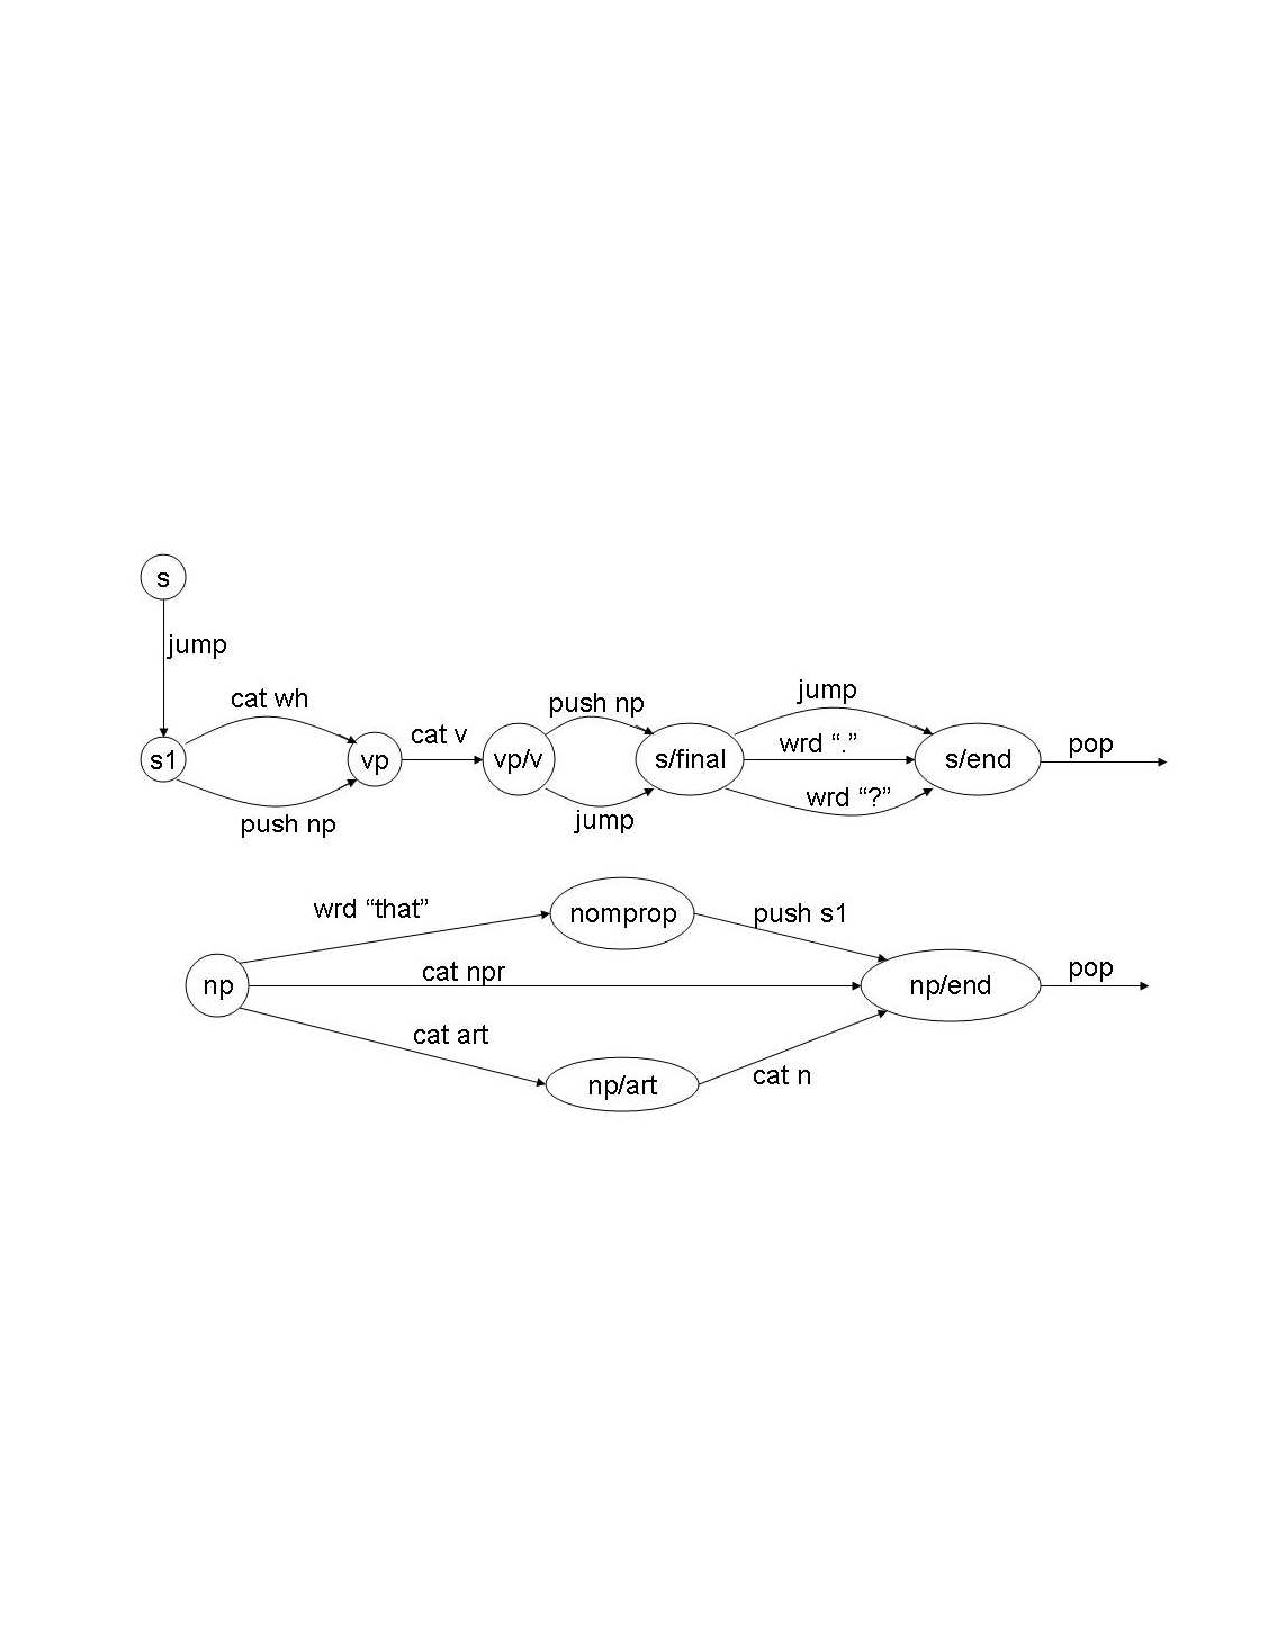
\includegraphics{gatn.pdf}}
\caption{Graphical version of the example GATN.}\label{gatnfig1}
\end{figure}
\begin{verbatim}
(s (jump s1 t (setf *parse-trees* t))) ; This initial arc is used to
                                ; set global variables and other parameters.

(s1 (cat wh t ; The only acceptable questions start with a wh word.
         (setr subj '(np \?)) (setr mood 'question) (to vp))
    (push np t ; The only acceptable statements are NP V [NP].
          (setr subj *) (setr mood 'decl) (to vp)))

(vp (cat v t (setr verb *) (to vp/v)))

(vp/v (push np t (setr obj *) (to s/final))
      (jump s/final t)) ; The predicate NP is optional.

(s/final (jump s/end (overlap embedded t)) ; The S might end with an embedded S.
         (wrd "." (overlap mood 'decl) (to s/end))
         (wrd "?" (overlap mood 'question) (to s/end)))

(s/end (pop (buildq (s (mood +) + (vp (v +))) mood subj verb) (nullr obj))
       (pop (buildq (s (mood +) + (vp (v +) +)) mood subj verb obj) obj))

(np (wrd "that" t (to nomprop)) ; An embedded S has "that" in front of it.
    (cat npr t (setr np (buildq (npr *))) (setr def t) (to np/end))
    (cat art t (setr def (getf definite)) (to np/art)))

(np/art (cat n t (setr np (buildq (n *))) (to np/end)))

(nomprop (push s1 t (sendr embedded t) (setr def t) (setr np *) (to np/end)))

(np/end (pop (buildq (np (definite +) +) def np) t))
\end{verbatim}

Here is the accompanying lexicon:
\begin{verbatim}
("a"                ((ctgy . art)(definite . nil)))
("the"              ((ctgy . art)(definite . t)))

("Computer Science" ((ctgy . npr)))
("John"             ((ctgy . npr)))
("Mary"             ((ctgy . npr)))

("computer"         ((ctgy . n)))
("Computer"         ((ctgy . multi-start) (multi-rest . ("Science")))
                    ((ctgy . n)(root . "computer")))
("dog"              ((ctgy . n)))
("man"              ((ctgy . n)(plur . "men")))
("men"              ((ctgy . n)(root . "man")(num . plur)))
("woman"            ((ctgy .  n)(plur . "women")))
("women"            ((ctgy . n)(root . "woman")(num . plur)))

("saw"              ((ctgy . n))
                    ((ctgy . v)(root . "see")(tense . past)))

("believe"          ((ctgy . v)(stative . t)))
("bit"              ((ctgy . v)(root . "bite")(tense . past)))
("bite"             ((ctgy . v)(num . plur)(past . "bit")))
("like"             ((ctgy . v)(num . plur)))
("see"              ((ctgy . v)(past . "saw")))
("sleep"            ((ctgy . v)(past . "slept")))
("slept"            ((ctgy . v)(root . "sleep")(tense . past))) 
("study"            ((ctgy . v)))
("use"              ((ctgy . v)))

("who"              ((ctgy . wh)))
("what"             ((ctgy . wh)))
\end{verbatim}
and here is a test run.  The output has been edited by changing some
line breaks and some indentation in order to show the parse
trees more clearly.
\begin{verbatim}
USER(29): (sneps)
   Welcome to SNePS-2.5 [PL:1 1999/08/19 16:38:25]

Copyright (C) 1984--1999 by Research Foundation of
State University of New York. SNePS comes with ABSOLUTELY NO WARRANTY!
Type `(copyright)' for detailed copyright information.
Type `(demo)' for a list of example applications.

   6/21/2002 9:51:59
* ^^
--> (atnin "grammar.lisp")
State S processed.
State S1 processed.
State VP processed.
State VP/V processed.
State S/OBJ processed.
State NP processed.
State NP/ART processed.
State NP/END1 processed.
State NP/END2 processed.
State S/END1 processed.
State S/END2 processed.
 Atnin read in states: (S/END2 S/END1 NP/END2 NP/END1 NP/ART NP S/OBJ VP/V VP
                        S1 S) 

--> (lexin "lexicon.lisp")
undefined- (NIL)
("a" "the" "some" "dog" "man" "men" "bite" "bites" "like" "likes")
--> (parse)
 ATN parser initialization... 
 Trace level = 0.
 Beginning at state 'S'.

 Input sentences in normal English orthographic convention. 
 Sentences may go beyond a line by having a space followed by a <CR>
 To exit the parser, write ^end.

 : A dog bit John.
Resulting parse:
(S (MOOD DECL)
   (NP (DEFINITE NIL) (N "dog"))
   (VP (V "bite")
       (NP (DEFINITE T) (NPR "John"))))
 Time (sec.): 0.05

 : The dog slept.
Resulting parse:
(S (MOOD DECL)
   (NP (DEFINITE T) (N "dog"))
   (VP (V "sleep")))
 Time (sec.): 0.05

 : Mary believes that John likes the dog.
Resulting parse:
(S (MOOD DECL)
   (NP (DEFINITE T) (NPR "Mary"))
   (VP (V "believe")
       (NP (DEFINITE T)
           (S (MOOD DECL)
              (NP (DEFINITE T) (NPR "John"))
              (VP (V "like")
                  (NP (DEFINITE T) (N "dog")))))))
 Time (sec.): 0.117

 : Mary studies Computer Science.
Resulting parse:
(S (MOOD DECL)
   (NP (DEFINITE T) (NPR "Mary"))
   (VP (V "study")
       (NP (DEFINITE T) (NPR "Computer Science"))))
 Time (sec.): 0.05

 : Mary used a computer.
Resulting parse:
(S (MOOD DECL)
   (NP (DEFINITE T) (NPR "Mary"))
   (VP (V "use")
       (NP (DEFINITE NIL) (N "computer"))))
 Time (sec.): 0.05
\end{verbatim}
\pagebreak
\begin{verbatim}
 : John saw a saw.
Resulting parse:
(S (MOOD DECL)
   (NP (DEFINITE T) (NPR "John"))
   (VP (V "see")
       (NP (DEFINITE NIL) (N "saw"))))
 Time (sec.): 0.067

 : What bit John?
Resulting parse:
(S (MOOD QUESTION)
   (NP ?)
   (VP (V "bite")
       (NP (DEFINITE T) (NPR "John"))))
 Time (sec.): 0.05

 : Who sleeps?
Resulting parse:
(S (MOOD QUESTION)
   (NP ?)
   (VP (V "sleep")))
 Time (sec.): 0.034

 : Who studied?
Resulting parse:
(S (MOOD QUESTION)
   (NP ?)
   (VP (V "study")))
 Time (sec.): 0.05

 : Who uses the computer?
Resulting parse:
(S (MOOD QUESTION)
   (NP ?)
   (VP (V "use")
       (NP (DEFINITE T) (N "computer"))))
 Time (sec.): 0.067

 : Who likes a dog?
Resulting parse:
(S (MOOD QUESTION)
   (NP ?)
   (VP (V "like")
       (NP (DEFINITE NIL) (N "dog"))))
 Time (sec.): 0.067
\end{verbatim}
\pagebreak
\begin{verbatim}
 : Who sees a saw?
Resulting parse:
(S (MOOD QUESTION)
   (NP ?)
   (VP (V "see")
       (NP (DEFINITE NIL) (N "saw"))))
 Time (sec.): 0.067
\end{verbatim}
 
\subsection{Interacting with SNePS}\label{nlkrxplsec}
The GATN in this section accepts the same fragment of English as the
one in the previous section, but, instead of building and returning
parse trees, it builds a SNePS network representing the information in
the statements and answers the questions.  The statements are echoed
and the questions are answered in English generated by the generation
part of this GATN.

\begin{verbatim}
;;; First, the SNePS relations used in the GATN are defined.
(^^ define agent act object propername member class lex)

;;; Next, a global variable, a global constant, and two functions are defined.
(^^ defvar *SaynBeforeVowels* nil
    "If true and the next word starts with a vowel,
     print 'n ' before that next word.")

(^^ defconstant *vowels* '(#\a #\e #\i #\o #\u)
    "A list of the vowels.")

;;; The following two functions implement a "phonological" component
;;; that can be used to output words and phrases from arcs of the GATN.
;;; In this way, the beginning of the sentence can be uttered before
;;; the rest of the sentence has been composed.

(^^ defun SayOneWord (word)
    "Prints the single WORD, which must be a string or a node.
     If the word is 'a', sets *SaynBeforeVowels*.
     If *SaynBeforeVowels* is set, then prints 'n ' before word/s
     if the first letter of word/s is a vowel."
    (check-type word (or string sneps:node))
    (when (sneps:node-p word) (setf word (format nil "~A" word)))
    (when *SaynBeforeVowels*
      (when (member (char word 0) *vowels* :test #'char=) (format t "n"))
      (setf *SaynBeforeVowels* nil))
    (when (string\= word "a") (setf *SaynBeforeVowels* t))
    (format t " ~A" word))

(^^ defun say (word/s)
    "Prints the single word or the list of words.
     If the word is 'a', sets *SaynBeforeVowels*.
     If *SaynBeforeVowels* is set, then prints 'n ' before word/s
     if the first letter of word/s is a vowel."
    (if (listp word/s) (mapc #'SayOneWord word/s)
        (SayOneWord word/s)))

;;; The initial arc is used to make two SNePSUL variables, each of
;;; which holds a SNePS variable node.  This results in a major
;;; efficiency gain over creating new SNePS variable nodes each time a
;;; question or an indefinite NP is parsed.
(s (jump s1 t 
         (or (* 'wh) ($ 'wh)) ; a SNePS variable to use for Wh questions
         (or (* 'x) ($ 'x)) ; a variable for indef NP's in questions
         ))
(s1 (push ps t                ; Parse a sentence, and send results to RESPOND
          (jump respond)))
(ps (cat wh t                        ; A Wh question starts with "who" or "what".
         (setr agent (* 'wh))        ; set AGENT to a variable node.
         (setr mood 'question) (liftr mood) (to vp))
    (push np t (sendr mood 'decl) ; The only acceptable statements are NP V [NP].
                                  ; MOOD must be sent down, because an indefinite
                                  ; NP introduces a new individual in a statement,
                                  ; but must be treated as a variable to be found
                                  ; in a question. 
          (setr agent *)        ; set AGENT to parse of subject.
          (setr mood 'decl) (liftr mood) ; The state RESPOND must know whether
                                         ; it is echoing a statement or answering
                                         ; a question.
          (to vp)))
(vp (cat v t                    ; Accept just a simple verb for this example,
         (setr act *) (to vp/v))) ; and ignore tense.
(vp/v (push np t (sendr mood)
            (setr object *)     ; Set OBJECT to parse of object.
            (to s/final))
      (jump s/final t))         ; If no object.

(s/final (jump s/end (overlap embedded t)) ; an embedded proposition
         (wrd "." (overlap mood 'decl) (to s/end))
         (wrd "?" (overlap mood 'question) (to s/end)))
(s/end (pop #!((assert agent ~(getr agent) ; Assert a top-level statement.
                       act   (build lex ~(getr act))
                       object ~(getr object)))
            (and (overlap mood 'decl) (nullr embedded)))
       (pop #2!((build agent ~(getr agent) ; Build an embedded statement.
                       act   (build lex ~(getr act))
                       object ~(getr object)))
            (and (getr embedded) (overlap mood 'decl)))
       (pop #!((deduce agent ~(getr agent) ; Use deduce to answer a question.
                       act   (build lex ~(getr act))
                       object ~(getr object)))
            (overlap mood 'question)))
;;; Notice in all three above arcs that if there is no object,
;;; (getr object) will evaluate to NIL,
;;; and the node will be built without an OBJECT arc.
\end{verbatim}
\pagebreak
\begin{verbatim}
(np (wrd "that" t (to nomprop))        ; an embedded proposition
    (cat npr t
         (setr head (or
                     ;; First try to find someone with the given name.
                     #!((find (compose object- ! propername) ~(getr *)))
                     ;; Otherwise, create one.
                     #!((find object-
                              (assert object #head propername ~(getr *))))))
         (to np/end))
    (cat art t (setr def (getf definite)) (to np/art)))

(np/art (cat n (overlap def t) ; a definite np
             (setr head ; Find the referent. (Assume there is exactly one.)
                   #!((find member-
                            (deduce member *x
                                    class (build lex ~(getr *))))))
             (to np/end))
        (cat n (and (disjoint def t) (overlap mood 'decl))
             (setr head        ; Create a new referent.
               #!((find member-
                        (assert member #hd
                          class (build lex ~(getr *))))))
             (to np/end))
        (cat n (and (disjoint def t) (overlap mood 'question))
             (setr head (* 'x)) ; a variable node.
             (to np/end)))

(nomprop (push ps t ; Return the parse of embedded sentence.
               (sendr embedded t) (setr head *) (to np/end)))

(np/end (pop head t))

;;;;;;;;;;;;;;;;;;;;;;
;;; Generation Section
;;;;;;;;;;;;;;;;;;;;;;

(respond (jump g (and (getr *) (overlap mood 'decl))
               (say "I understand that")) ; Canned beginning of echo of statement.
         (jump g (and (getr *) (overlap mood 'question))) ; Answer of question.
         (jump g/end (nullr *) (say "I don't know."))) ; Question not answered.

(g (rcall gnp (geta agent) (geta agent) ; Generate the agent as an np.
          reg (jump g/subj)))

(g/subj (jump g/v (geta act)
              (say (verbize 'past ; For this example, always use past tense.
                            (first (geta lex (geta act)))))))

(g/v (rcall gnp (geta object) (geta object) ; Generate the object.
            reg (to g/end))
     (to (g/end) (null (geta object)))) ; No object.

(g/end (pop nil t))

(gnp (to (gnp/end) (geta propername (geta object-))
         (say (geta propername (geta object-)))) ; Generate an npr.
     (to (gnp/end) (geta class (geta member-)) ; An indef np.
         (say (cons "a" #!((find (lex- class- ! member) ~(getr *))))))
     (call g * (geta act) (say "that") * ; An embedded proposition
           (to gnp/end)))

(gnp/end (pop nil t))
\end{verbatim}

Here is a sample run using this grammar and the same lexicon as before:
\begin{verbatim}
--> (parse)
 ATN parser initialization... 
 Trace level = 0.
 Beginning at state 'S'.

 Input sentences in normal English orthographic convention. 
 Sentences may go beyond a line by having a space followed by a <CR>
 To exit the parser, write ^end.

 : A dog bit John.
 I understand that a dog bit John
 Time (sec.): 0.25

 : The dog slept.
 I understand that a dog slept
 Time (sec.): 1.884

 : Mary believes that John likes the dog.
 I understand that Mary believed that John liked a dog
 Time (sec.): 0.4

 : Mary studies Computer Science.
 I understand that Mary studied Computer Science
 Time (sec.): 0.2

 : Mary used a computer.
 I understand that Mary used a computer
 Time (sec.): 0.233

 : John saw a saw.
 I understand that John saw a saw
 Time (sec.): 0.217

 : What bit John?
 a dog bit John
 Time (sec.): 0.167
\end{verbatim}
\pagebreak
\begin{verbatim}
 : Who sleeps?
 a dog slept
 Time (sec.): 0.917

 : Who studied?
 Mary studied
 Time (sec.): 0.167

 : Who uses the computer?
 Mary used a computer
 Time (sec.): 0.267

 : Who likes a dog?
 I don't know.
 Time (sec.): 0.167

 : Who sees a saw?
 John saw a saw
 Time (sec.): 0.217
\end{verbatim}

The SNePS network built as a result of this interaction is shown in
Figure~\ref{gatnfig2}.  Note especially that when definite noun
phrases occurred in statements, they were represented by nodes that
were already in the net because of previous indefinite noun phrases.
\begin{figure}[tbp]
\vspace{1in}
%\resizebox{\textwidth}{!}{\includegraphics{netfig.ps}}
\resizebox{\textwidth}{!}{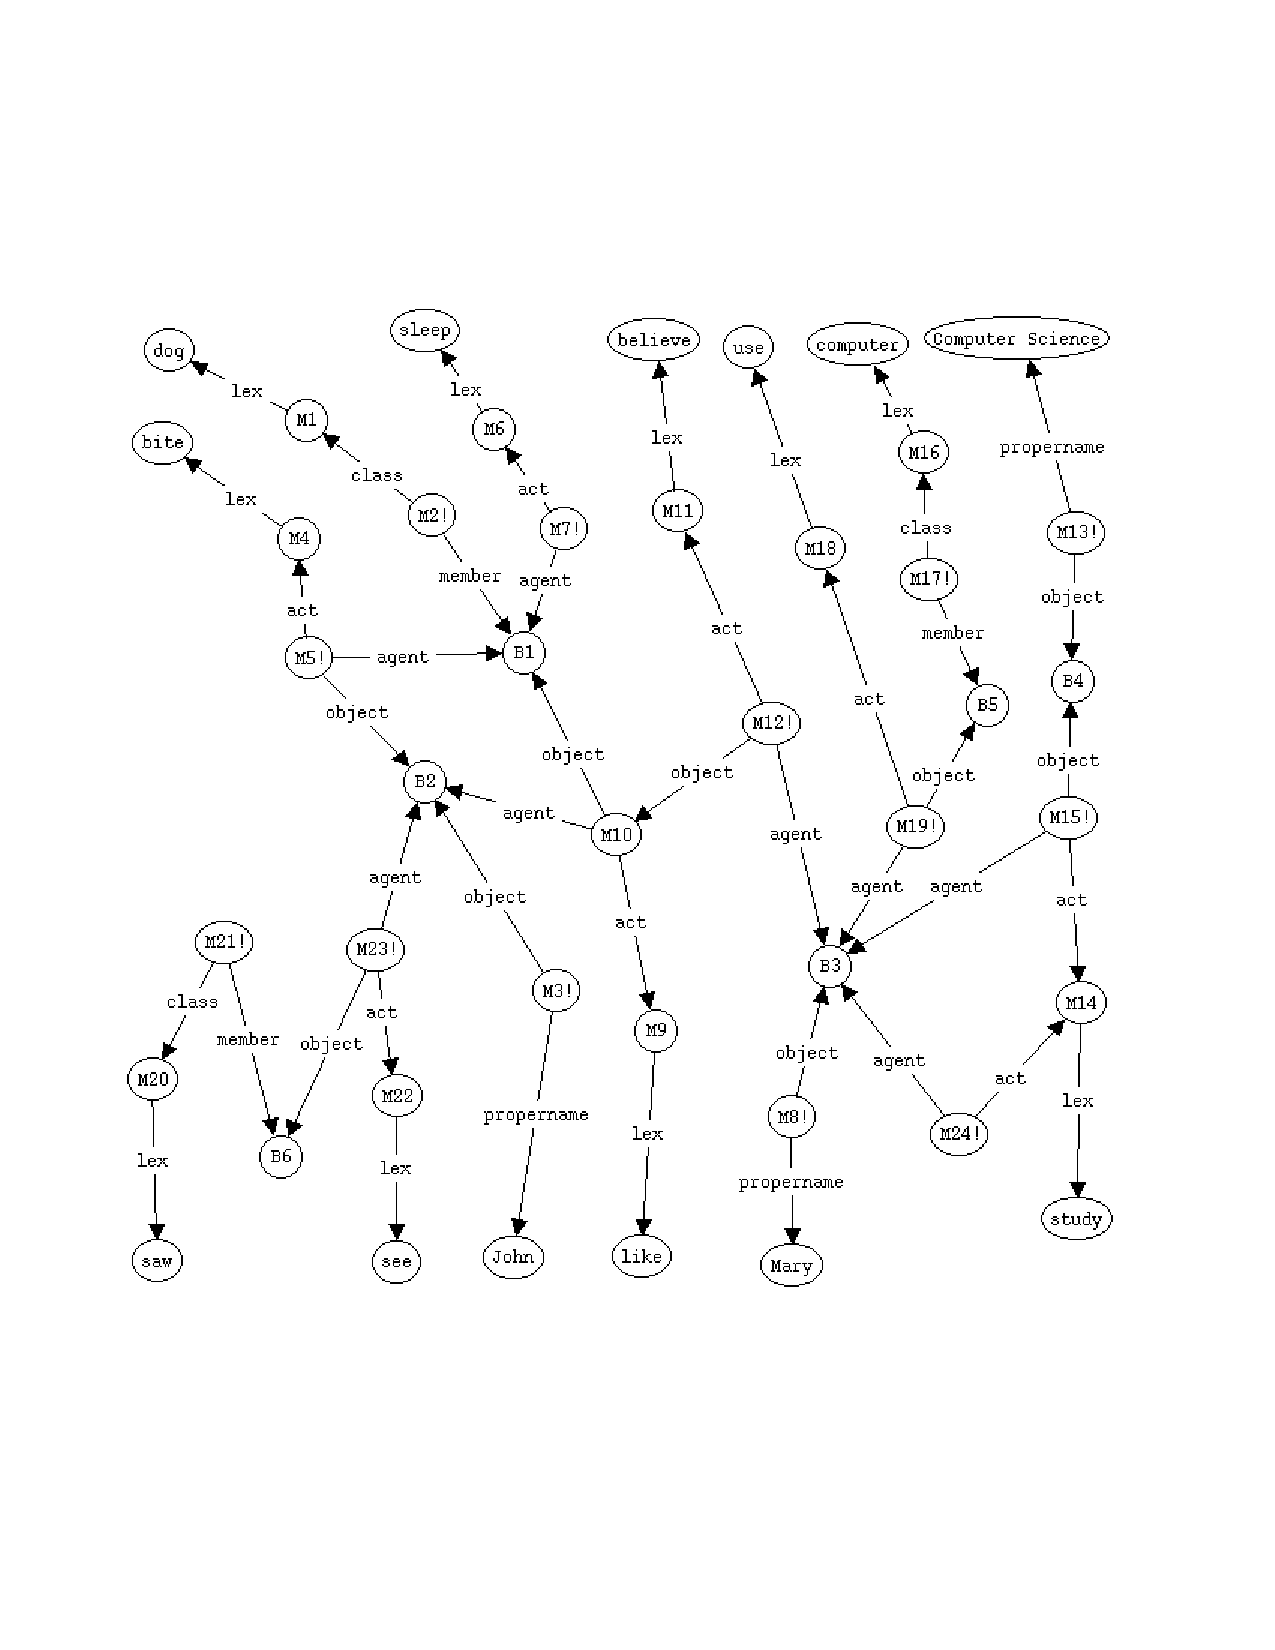
\includegraphics{netfig.pdf}}
\caption{SNePS network after running the example.}\label{gatnfig2}
\end{figure}


\chapter{SNePS as a Database Management System}
SNePS can be used as a network version of a relational database system
in which every element of the relational database is represented by a
base node, each row of each relation is represented by a molecular
node, and each column label (attribute) is represented by an arc
label.  Whenever a row $r$ of a relation $R$ has an element $e_i$ in
column $c_i,$ the molecular node representing $r$ has an arc labeled
$R$ to the special node {\tt relation}, and an arc labelled $c_i$
pointing to the base node representing $e_i.$ Table~\ref{dbtable}
shows two relations from the Supplier-Part-Project database of
Date\footnote{C. J. Date, {\em An Introduction to Database Systems 3rd
Edition} (Reading, MA: Addison-Wesley) 1981.}, p. 114.
\begin{table}[htb]
\caption{From Date's Supplier-Part-Project Database}\label{dbtable}
\begin{center}
\begin{tabular}{|l|l|c|l|}
\multicolumn{4}{l}{\bf SUPPLIER}\\\hline
S\# & SNAME & STATUS & CITY \\\hline
s1 & Smith & 20 & London\\
s2 & Jones & 10 & Paris\\
s3 & Blake & 30 & Paris\\
s4 & Clark & 20 & London\\
s5 & Adams & 30 & Athens\\\hline
\end{tabular} \hspace{0.5in}
\begin{tabular}{|l|l|l|}
\multicolumn{3}{l}{\bf PROJECT}\\\hline
J\# & JNAME & CITY\\\hline
j1 & sorter & Paris\\
j2 & punch & Rome\\
j3 & reader & Athens\\
j4 & console & Athens\\
j5 & collator & London\\
j6 & terminal & Oslo\\
j7 & tape & London\\\hline
\end{tabular}
\end{center}
\end{table}
Figure~\ref{dbfig1} shows a fragment of the SNePS network version of
this database.
\begin{figure}[tbp]
%\resizebox{\textwidth}{!}{\includegraphics{fig8a.ps}}
\resizebox{\textwidth}{!}{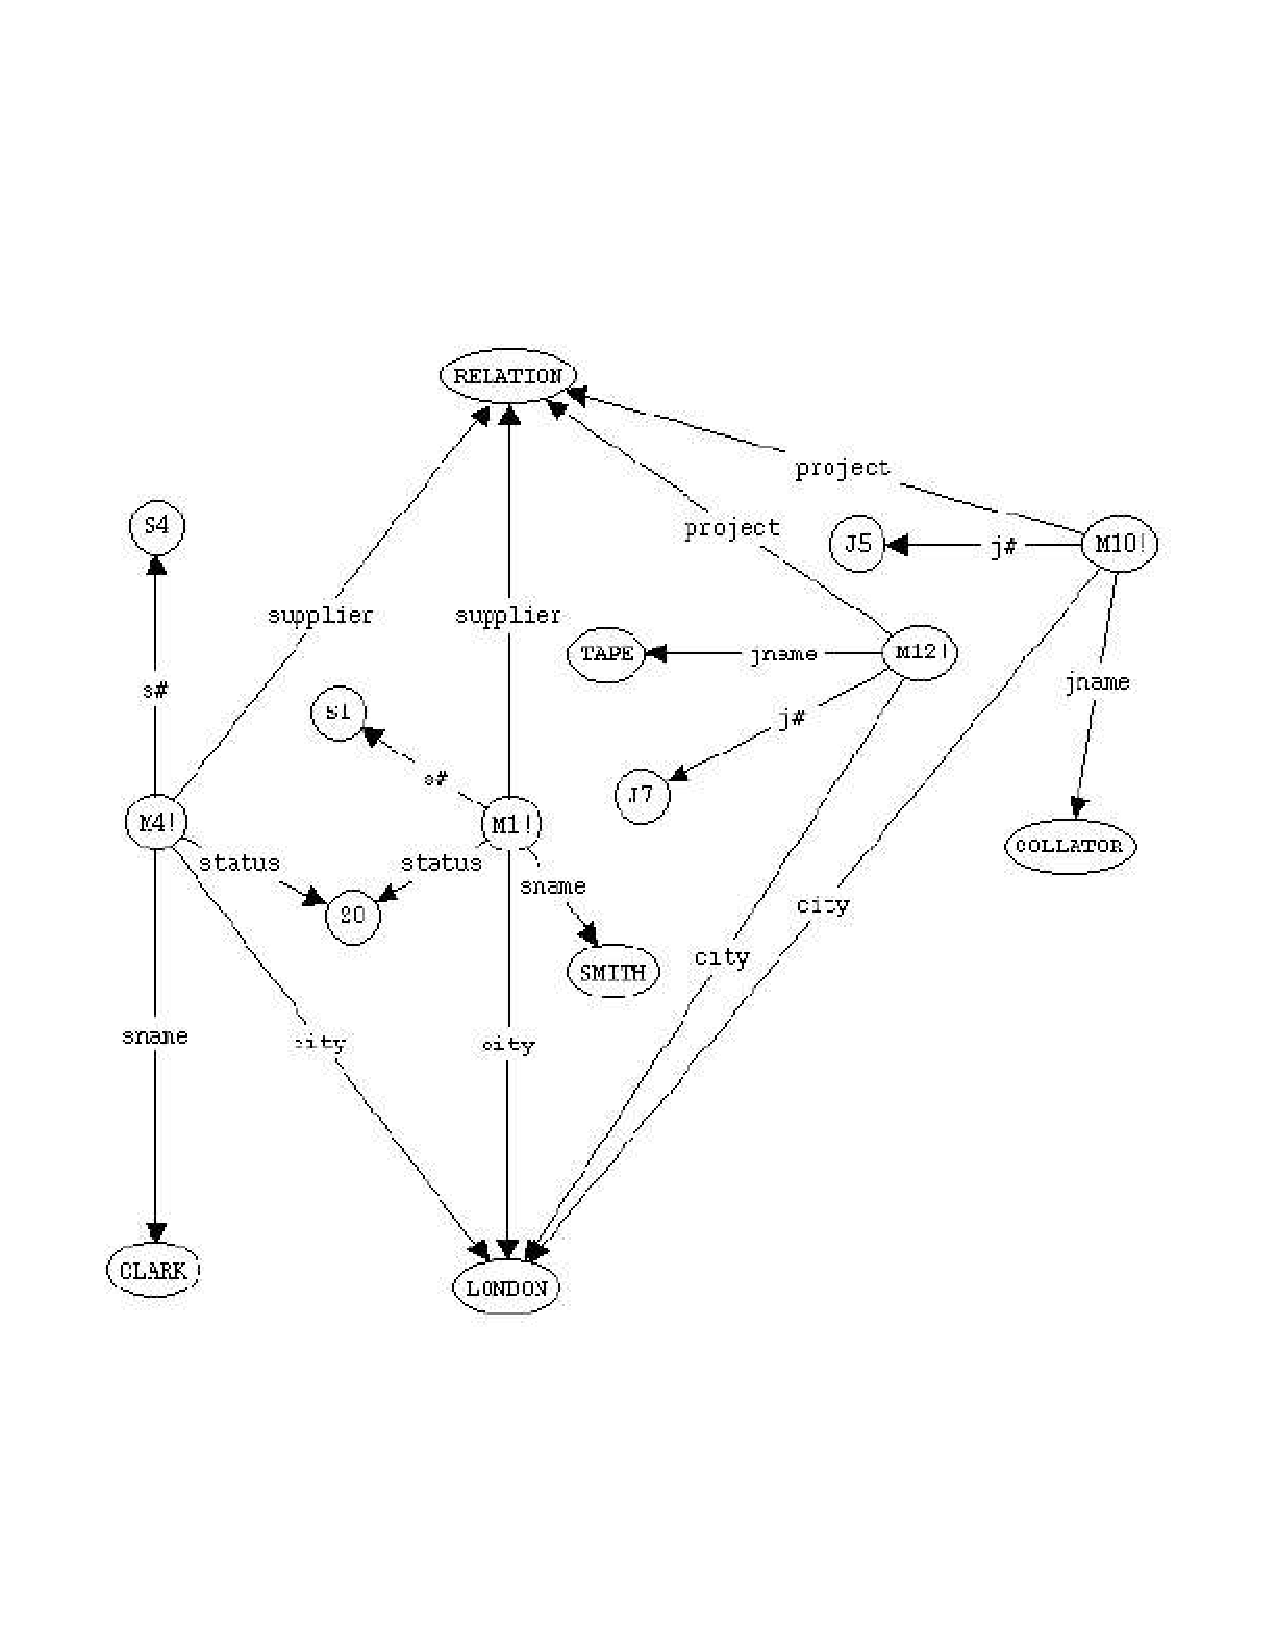
\includegraphics{fig8a.pdf}}
\caption{Fragment of SNePS network for the Supplier-Part-Project
Database}\label{dbfig1} 
\end{figure}

\section{SNePS as a Relational Database}
The three basic operations on relational databases are {\bf select,
project,} and {\bf join.}  The next three subsections show how these
operations may be expressed in SNePSUL.

\subsection{Project}
{\bf Project} is a database operation that, given one relation,
produces another that has all the rows of the first, but only specific
columns.  (Actually some of the rows might collapse if the only
distinguishing elements were in columns that were eliminated.)  The
SNePSUL {\tt dbproject} function has been designed for this purpose.
For example, to show the STATUS and CITY of all suppliers, one can do
\begin{verbatim}
* (dbproject (find supplier relation) status city)
((STATUS (20) CITY (LONDON)) (STATUS (10) CITY (PARIS))
 (STATUS (30) CITY (PARIS)) (STATUS (30) CITY (ATHENS)))
 CPU time : 0.07 
\end{verbatim}

The {\tt dbproject} function forms and returns a {\em virtual}
relation, which is represented as a SNePS data type called a {\em set
of flat cable sets.}  Compare the following two ways of getting
complete details of the SUPPLIER relation.  The first uses the SNePSUL
{\tt describe} function to print the details of the nodes that make up
the relation:
\begin{verbatim}
* (describe (find supplier relation))
(M1! (CITY LONDON) (S# S1) (SNAME SMITH) (STATUS 20) (SUPPLIER RELATION))
(M2! (CITY PARIS) (S# S2) (SNAME JONES) (STATUS 10) (SUPPLIER RELATION))
(M3! (CITY PARIS) (S# S3) (SNAME BLAKE) (STATUS 30) (SUPPLIER RELATION))
(M4! (CITY LONDON) (S# S4) (SNAME CLARK) (STATUS 20) (SUPPLIER RELATION))
(M5! (CITY ATHENS) (S# S5) (SNAME ADAMS) (STATUS 30) (SUPPLIER RELATION))
(M1! M2! M3! M4! M5!)
 CPU time : 0.15 
\end{verbatim}
The second uses {\tt dbproject} to display a virtual relation with the
same information:
\begin{verbatim}
* (dbproject (find supplier relation) supplier s\# sname status city)
((SUPPLIER (RELATION) S# (S1) SNAME (SMITH) STATUS (20) CITY (LONDON))
 (SUPPLIER (RELATION) S# (S2) SNAME (JONES) STATUS (10) CITY (PARIS))
 (SUPPLIER (RELATION) S# (S3) SNAME (BLAKE) STATUS (30) CITY (PARIS))
 (SUPPLIER (RELATION) S# (S4) SNAME (CLARK) STATUS (20) CITY (LONDON))
 (SUPPLIER (RELATION) S# (S5) SNAME (ADAMS) STATUS (30) CITY (ATHENS)))
 CPU time : 0.12 
\end{verbatim}

Virtual relations are created without building any new SNePS network
structure.  To make these relations permanent, use the SNePSUL {\tt
dbAssertVirtual} function.  For example, to create a CITYSTATUS
relation that is a projection of the SUPPLIER relation down the CITY
and STATUS attributes, we would first define CITYSTATUS as a new SNePS
relation:
\begin{verbatim}
* (define citystatus)
(CITYSTATUS)
 CPU time : 0.03 
\end{verbatim}
Then we would do
\begin{verbatim}
* (describe (dbAssertVirtual (dbproject (find supplier relation) city status) 
                             (citystatus relation)))
(M13! (CITY LONDON) (CITYSTATUS RELATION) (STATUS 20))
(M14! (CITY PARIS) (CITYSTATUS RELATION) (STATUS 10))
(M15! (CITY PARIS) (CITYSTATUS RELATION) (STATUS 30))
(M16! (CITY ATHENS) (CITYSTATUS RELATION) (STATUS 30))
(M13! M14! M15! M16!)
 CPU time : 0.28 
\end{verbatim}

\subsection{Select}
{\bf Select} is an operation that is given a relation and specific
values for some of its attributes, and yields the rows of the
relations in which those attributes take on those values.  A selection
from relation $R_1$ in which attribute $a_{1i}$ takes on value
$v_{1i}$ is expressed in SNePSUL as
\begin{center}
{\tt (find $R_1$ relation $a_{11}$ $v_{11}$ \ldots $a_{1n}$ $v_{1n}$)}.
\end{center}
For example, to select rows of the SUPPLIER relation where the CITY is
Paris or Athens and the STATUS is 30, we could do:
\begin{verbatim}
* (describe (find supplier relation city (paris athens) status 30))
(M3! (CITY PARIS) (S# S3) (SNAME BLAKE) (STATUS 30) (SUPPLIER RELATION))
(M5! (CITY ATHENS) (S# S5) (SNAME ADAMS) (STATUS 30) (SUPPLIER RELATION))
(M3! M5!)
 CPU time : 0.08
\end{verbatim}
If we want a new permanent relation, say {\tt supplier2}, to be this
selection from the SUPPLIER relation, we could do:
\begin{verbatim}
* (define supplier2)
(SUPPLIER2)
 CPU time : 0.03 

* (describe
   (dbAssertVirtual
    (dbproject (find supplier relation city (paris athens) status 30)
               s\# sname status city)
    (supplier2 relation)))
(M17! (CITY PARIS) (S# S3) (SNAME BLAKE) (STATUS 30) (SUPPLIER2 RELATION))
(M18! (CITY ATHENS) (S# S5) (SNAME ADAMS) (STATUS 30) (SUPPLIER2 RELATION))
(M17! M18!)
 CPU time : 0.23 
\end{verbatim}

\subsection{Join}
{\bf Join} is a database operation that, given two relations, $R_1$ and
$R_2$, with attributes $a_{11}, \ldots, a_{1n}$ and $a_{21}, \ldots,
a_{2m}$, respectively, and an atttibute $a=a_{1i}=a_{2j}$ produces a
relation with attributes $a_{11}, \ldots, a_{1n}, a_{21}, \ldots,
a_{2j-1}, a_{2j+1}, \ldots, a_{2m}$, and every row, $e_{11}, \ldots,
e_{1n}, e_{21}, \ldots, e_{2j-1}, e_{2j+1}, \ldots, e_{2m}$ where
$e_{11}, \ldots, e_{1n}$ was a row of $R_1$, and $e_{21}, \ldots,
e_{2j-1}, e_{1i}, e_{2j+1}, \ldots, e_{2m}$ was a row of $R_2$.  For
example, Table~\ref{dbtable2} shows the join of the relations in
Table~\ref{dbtable} on the attribute CITY.
\begin{table}[htb]
\caption{The join of SUPPLIER and PROJECT on CITY}\label{dbtable2}
\begin{center}
\begin{tabular}{|l|l|c|l|l|l|}\hline
S\# & SNAME & STATUS & CITY & J\# & JNAME\\\hline
s1 & Smith & 20 & London & j5 & collator\\
s1 & Smith & 20 & London & j7 & tape\\
s2 & Jones & 10 & Paris & j1 & sorter\\
s3 & Blake & 30 & Paris & j1 & sorter\\
s4 & Clark & 20 & London & j5 & collator\\
s4 & Clark & 20 & London & j7 & tape\\
s5 & Adams & 30 & Athens & j3 & reader\\
s5 & Adams & 30 & Athens & j4 & console\\\hline
\end{tabular} \hspace{0.5in}
\end{center}
\end{table}

This join may be created and displayed by the SNePSUL {\tt dbjoin}
command, which, like\\ {\tt dbproject} creates a virtual relation.
\begin{verbatim}
* (dbjoin city
          (find supplier relation) (s\# sname status city)
          (find project relation) (j\# jname))
(S# (S1) SNAME (SMITH) STATUS (20) CITY (LONDON) J# (J7) JNAME (TAPE))
(S# (S1) SNAME (SMITH) STATUS (20) CITY (LONDON) J# (J5) JNAME (COLLATOR))
(S# (S2) SNAME (JONES) STATUS (10) CITY (PARIS) J# (J1) JNAME (SORTER))
(S# (S3) SNAME (BLAKE) STATUS (30) CITY (PARIS) J# (J1) JNAME (SORTER))
(S# (S4) SNAME (CLARK) STATUS (20) CITY (LONDON) J# (J7) JNAME (TAPE))
(S# (S4) SNAME (CLARK) STATUS (20) CITY (LONDON) J# (J5) JNAME (COLLATOR))
(S# (S5) SNAME (ADAMS) STATUS (30) CITY (ATHENS) J# (J4) JNAME (CONSOLE))
(S# (S5) SNAME (ADAMS) STATUS (30) CITY (ATHENS) J# (J3) JNAME (READER))
 CPU time : 0.35 
\end{verbatim}

Again, to make the virtual relation permanent, {\tt dbAssertVirtual}
is used:
\begin{verbatim}
* (define supplierproject)
(SUPPLIERPROJECT)
 CPU time : 0.03 

* (describe
   (dbAssertVirtual
    (dbjoin city
            (find supplier relation) (s\# sname status city)
            (find project relation) (j\# jname))
    (supplierproject relation)))
(M19! (CITY LONDON) (J# J7) (JNAME TAPE) (S# S1) (SNAME SMITH) (STATUS 20)
      (SUPPLIERPROJECT RELATION))
(M20! (CITY LONDON) (J# J5) (JNAME COLLATOR) (S# S1) (SNAME SMITH) (STATUS 20)
      (SUPPLIERPROJECT RELATION))
(M21! (CITY PARIS) (J# J1) (JNAME SORTER) (S# S2) (SNAME JONES) (STATUS 10)
      (SUPPLIERPROJECT RELATION))
(M22! (CITY PARIS) (J# J1) (JNAME SORTER) (S# S3) (SNAME BLAKE) (STATUS 30)
      (SUPPLIERPROJECT RELATION))
(M23! (CITY LONDON) (J# J7) (JNAME TAPE) (S# S4) (SNAME CLARK) (STATUS 20)
      (SUPPLIERPROJECT RELATION))
(M24! (CITY LONDON) (J# J5) (JNAME COLLATOR) (S# S4) (SNAME CLARK) (STATUS 20)
      (SUPPLIERPROJECT RELATION))
(M25! (CITY ATHENS) (J# J4) (JNAME CONSOLE) (S# S5) (SNAME ADAMS) (STATUS 30)
      (SUPPLIERPROJECT RELATION))
(M26! (CITY ATHENS) (J# J3) (JNAME READER) (S# S5) (SNAME ADAMS) (STATUS 30)
      (SUPPLIERPROJECT RELATION))
(M19! M20! M21! M22! M23! M24! M25! M26!)
 CPU time : 0.92 
\end{verbatim}


\section{SNePS as a Network Database}
Although SNePS can be treated as a relational database, as shown in
the previous section, it is more naturally a network database.  For
example, to find the names of suppliers with the same status as
suppliers in the same city as the sorter project using relational
database techniques, one would join the SUPPLIER and PROJECT relations
on CITY, join the result with SUPPLIER again on STATUS, select rows
where PROJECT is sorter, and project the result on the SNAME
attribute.

However, in SNePSUL, one could just do
\begin{verbatim}
* (find (sname- status status- city city- jname) sorter)
(ADAMS BLAKE JONES)
 CPU time : 0.02 
\end{verbatim}
Additional examples of these techniques may be found in the SNePS DBMS
demonstration.

\section{Database Functions}
Functions specifically supplied for treating SNePS as a Database
Management System are documented in this section.  Additional ones may
be created using the functions documented in
Chapter~\ref{interfacechap}.  Note also {\tt innet} and {\tt outnet},
documented in Section~\ref{filesec}, for saving the database across
runs.

\docfun{dbAssertVirtual}{{\it virtualexp} [([{\it relation nodeset\/}]$^*$)]}
Evaluates {\it virtualexp}, which must return a virtual relation (set
of flat cable sets), appends the list {\tt ([{\it relation
nodeset\/}]$^*$)} to each flat cable set, asserts each resulting flat
cable set as a SNePS molecular node, and returns the set of asserted
nodes.


\docfun{dbcount}{{\it nodesetexp}}
Evaluates the SNePSUL nodeset expression, {\it nodesetexp},
and returns a node whose identifier looks like the number which is
the number of nodes in the resulting set.

\docfun{dbjoin}{{\it relation nodesetexp1 relations1 nodesetexp2
relations2}} A virtual relation (a set of flat cable sets) is created and
returned.  The virtual relation is formed by taking the nodes returned
by the SNePSUL node set expression, {\it nodesetexp1} and the nodes
returned by the SNePSUL node set expression, {\it nodesetexp2,}
joining these two relations on the attribute {\it relation,} and then
projecting the result down the {\it relations1} attributes from the
first nodeset and the {\it relations2} attributes from the second
nodeset.  Note that {\tt relations1} and {\tt relations2} is each a
list of relations.

\docfun{dbmax}{{\it nodesetexp}}
Evaluates the SNePSUL nodeset expression, {\it nodesetexp}, which must
evaluate to a set of nodes all of whose identifiers look like numbers,
and returns the node whose identifier looks like the biggest of the
numbers.

\docfun{dbmin}{{\it nodesetexp}}
Evaluates the SNePSUL nodeset expression, {\it nodesetexp}, which must
evaluate to a set of nodes all of whose identifiers look like numbers,
and returns the node whose identifier looks like the smallest of the
numbers.

\docfun{dbproject}{{\it nodesetexp relations}}
A virtual relation (a set of flat cable sets) is created and returned.  The
virtual relation is formed by taking the nodes returned by the SNePSUL
node set expression, {\it nodesetexp,} and projecting down the SNePSUL
relations included in the sequence, {\it relations}.

\docfun{dbtot}{{\it nodesetexp}}
Evaluates the SNePSUL nodeset expression, {\it nodesetexp}, which must
evaluate to a set of nodes all of whose identifiers look like numbers,
and returns a node whose identifier looks like the sum of the numbers.


\backmatter
\appendix

\chapter{University at Buffalo Public License (``UBPL'') Version 1.0}
\renewcommand{\thesection}{\arabic{section}.}
\renewcommand{\thesubsection}{\arabic{section}.\arabic{subsection}.}
\setcounter{section}{0}
\section{Definitions.}
\begin{description}
\item [1.0.1. ``Commercial Use'']\mbox{}\\
means distribution or otherwise making the Covered Code available to a third party. 
\item [1.1. ``Contributor'']\mbox{}\\
means each entity that creates or contributes to the creation of Modifications. 
\item [1.2. ``Contributor Version'']\mbox{}\\
means the combination of the Original Code, prior Modifications used by a Contributor, and the Modifications made by that particular Contributor. 
\item [1.3. ``Covered Code'']\mbox{}\\
means the Original Code or Modifications or the combination of the Original Code and Modifications, in each case including portions thereof. 
\item [1.4. ``Electronic Distribution Mechanism'']\mbox{}\\
means a mechanism generally accepted in the software development community for the electronic transfer of data. 
\item [1.5. ``Executable'']\mbox{}\\
means Covered Code in any form other than Source Code. 
\item [1.6. ``Initial Developer'']\mbox{}\\
means the individual or entity identified as the Initial Developer in the Source Code notice required by Exhibit A. 
\item [1.7. ``Larger Work'']\mbox{}\\
means a work which combines Covered Code or portions thereof with code not governed by the terms of this License. 
\item [1.8. ``License'']\mbox{}\\
means this document. 
\item [1.8.1. ``Licensable'']\mbox{}\\
means having the right to grant, to the maximum extent possible, whether at the time of the initial grant or subsequently acquired, any and all of the rights conveyed herein. 
\item [1.9. ``Modifications'']\mbox{}\\
means any addition to or deletion from the substance or structure of either the Original Code or any previous Modifications. When Covered Code is released as a series of files, a Modification is: 
\renewcommand{\theenumi}{\alph{enumi}}
\begin{enumerate}
\item Any addition to or deletion from the contents of a file containing Original Code or previous Modifications. 
\item Any new file that contains any part of the Original Code or previous Modifications. 
\end{enumerate}

\item [1.10. ``Original Code'']\mbox{}\\
means Source Code of computer software code which is described in the Source Code notice required by Exhibit A as Original Code, and which, at the time of its release under this License is not already Covered Code governed by this License. 

\item [1.10.1. ``Patent Claims'']\mbox{}\\
means any patent claim(s), now owned or hereafter acquired, including without limitation, method, process, and apparatus claims, in any patent Licensable by grantor. 
\item [1.11. ``Source Code'']\mbox{}\\
means the preferred form of the Covered Code for making modifications to it, including all modules it contains, plus any associated interface definition files, scripts used to control compilation and installation of an Executable, or source code differential comparisons against either the Original Code or another well known, available Covered Code of the Contributor's choice. The Source Code can be in a compressed or archival form, provided the appropriate decompression or de-archiving software is widely available for no charge. 
\item [1.12. ``You'' (or ``Your'')]\mbox{}\\
means an individual or a legal entity exercising rights under, and complying with all of the terms of, this License or a future version of this License issued under Section 6.1. For legal entities, ``You'' includes any entity which controls, is controlled by, or is under common control with You. For purposes of this definition, ``control'' means (a) the power, direct or indirect, to cause the direction or management of such entity, whether by contract or otherwise, or (b) ownership of more than fifty percent (50\%) of the outstanding shares or beneficial ownership of such entity. 
\end{description}

\section{Source Code License.}
\subsection{The Initial Developer Grant.}
The Initial Developer hereby grants You a world-wide, royalty-free, non-exclusive license, subject to third party intellectual property claims: 
\renewcommand{\theenumi}{\alph{enumi}}
\begin{enumerate}
\item under intellectual property rights (other than patent or trademark) Licensable by Initial Developer to use, reproduce, modify, display, perform, sublicense and distribute the Original Code (or portions thereof) with or without Modifications, and/or as part of a Larger Work; and 

\item under Patents Claims infringed by the making, using or selling of Original Code, to make, have made, use, practice, sell, and offer for sale, and/or otherwise dispose of the Original Code (or portions thereof). 

\item the licenses granted in this Section 2.1 (a) and (b) are effective on the date Initial Developer first distributes Original Code under the terms of this License. 

\item Notwithstanding Section 2.1 (b) above, no patent license is granted: 1) for code that You delete from the Original Code; 2) separate from the Original Code; or 3) for infringements caused by: i) the modification of the Original Code or ii) the combination of the Original Code with other software or devices. 
\end{enumerate}


\subsection{Contributor Grant.}
Subject to third party intellectual property claims, each Contributor hereby grants You a world-wide, royalty-free, non-exclusive license 
\begin{enumerate}
\item under intellectual property rights (other than patent or trademark) Licensable by Contributor, to use, reproduce, modify, display, perform, sublicense and distribute the Modifications created by such Contributor (or portions thereof) either on an unmodified basis, with other Modifications, as Covered Code and/or as part of a Larger Work; and 

\item under Patent Claims infringed by the making, using, or selling
  of Modifications made by that Contributor either alone and/or in
  combination with its Contributor Version (or portions of such
  combination), to make, use, sell, offer for sale, have made, and/or
  otherwise dispose of: 1) Modifications made by that Contributor (or
  portions thereof); and 2) the combination of Modifications made by
  that Contributor with its Contributor Version (or portions of such
  combination). 

\item the licenses granted in Sections 2.2 (a) and 2.2 (b) are effective on the date Contributor first makes Commercial Use of the Covered Code. 

\item Notwithstanding Section 2.2 (b) above, no patent license is granted: 1) for any code that Contributor has deleted from the Contributor Version; 2) separate from the Contributor Version; 3) for infringements caused by: i) third party modifications of Contributor Version or ii) the combination of Modifications made by that Contributor with other software (except as part of the Contributor Version) or other devices; or 4) under Patent Claims infringed by Covered Code in the absence of Modifications made by that Contributor. 
\end{enumerate}

\section{Distribution Obligations.}
\subsection{Application of License.}
The Modifications which You create or to which You contribute are governed by the terms of this License, including without limitation Section 2.2. The Source Code version of Covered Code may be distributed only under the terms of this License or a future version of this License released under Section 6.1, and You must include a copy of this License with every copy of the Source Code You distribute. You may not offer or impose any terms on any Source Code version that alters or restricts the applicable version of this License or the recipients' rights hereunder. However, You may include an additional document offering the additional rights described in Section 3.5. 

\subsection{Availability of Source Code.}
Any Modification which You create or to which You contribute must be made available in Source Code form under the terms of this License either on the same media as an Executable version or via an accepted Electronic Distribution Mechanism to anyone to whom you made an Executable version available; and if made available via Electronic Distribution Mechanism, must remain available for at least twelve (12) months after the date it initially became available, or at least six (6) months after a subsequent version of that particular Modification has been made available to such recipients. You are responsible for ensuring that the Source Code version remains available even if the Electronic Distribution Mechanism is maintained by a third party. 

\subsection{Description of Modifications.}
You must cause all Covered Code to which You contribute to contain a file documenting the changes You made to create that Covered Code and the date of any change. You must include a prominent statement that the Modification is derived, directly or indirectly, from Original Code provided by the Initial Developer and including the name of the Initial Developer in (a) the Source Code, and (b) in any notice in an Executable version or related documentation in which You describe the origin or ownership of the Covered Code. 

\subsection{Intellectual Property Matters}
\subsubsection{(a) Third Party Claims}
If Contributor has knowledge that a license under a third party's intellectual property rights is required to exercise the rights granted by such Contributor under Sections 2.1 or 2.2, Contributor must include a text file with the Source Code distribution titled ``LEGAL'' which describes the claim and the party making the claim in sufficient detail that a recipient will know whom to contact. If Contributor obtains such knowledge after the Modification is made available as described in Section 3.2, Contributor shall promptly modify the LEGAL file in all copies Contributor makes available thereafter and shall take other steps (such as notifying appropriate mailing lists or newsgroups) reasonably calculated to inform those who received the Covered Code that new knowledge has been obtained. 

\subsubsection{(b) Contributor APIs}
If Contributor's Modifications include an application programming interface and Contributor has knowledge of patent licenses which are reasonably necessary to implement that API, Contributor must also include this information in the LEGAL file. 

\subsubsection{(c) Representations.}
Contributor represents that, except as disclosed pursuant to Section 3.4 (a) above, Contributor believes that Contributor's Modifications are Contributor's original creation(s) and/or Contributor has sufficient rights to grant the rights conveyed by this License. 

\subsection{Required Notices.}
You must duplicate the notice in Exhibit A in each file of the Source Code. If it is not possible to put such notice in a particular Source Code file due to its structure, then You must include such notice in a location (such as a relevant directory) where a user would be likely to look for such a notice. If You created one or more Modification(s) You may add your name as a Contributor to the notice described in Exhibit A. You must also duplicate this License in any documentation for the Source Code where You describe recipients' rights or ownership rights relating to Covered Code. You may choose to offer, and to charge a fee for, warranty, support, indemnity or liability obligations to one or more recipients of Covered Code. However, You may do so only on Your own behalf, and not on behalf of the Initial Developer or any Contributor. You must make it absolutely clear than any such warranty, support, indemnity or liability obligation is offered by You alone, and You hereby agree to indemnify the Initial Developer and every Contributor for any liability incurred by the Initial Developer or such Contributor as a result of warranty, support, indemnity or liability terms You offer. 

\subsection{Distribution of Executable Versions.}
You may distribute Covered Code in Executable form only if the requirements of Sections 3.1, 3.2, 3.3, 3.4 and 3.5 have been met for that Covered Code, and if You include a notice stating that the Source Code version of the Covered Code is available under the terms of this License, including a description of how and where You have fulfilled the obligations of Section 3.2. The notice must be conspicuously included in any notice in an Executable version, related documentation or collateral in which You describe recipients' rights relating to the Covered Code. You may distribute the Executable version of Covered Code or ownership rights under a license of Your choice, which may contain terms different from this License, provided that You are in compliance with the terms of this License and that the license for the Executable version does not attempt to limit or alter the recipient's rights in the Source Code version from the rights set forth in this License. If You distribute the Executable version under a different license You must make it absolutely clear that any terms which differ from this License are offered by You alone, not by the Initial Developer or any Contributor. You hereby agree to indemnify the Initial Developer and every Contributor for any liability incurred by the Initial Developer or such Contributor as a result of any such terms You offer. 

\subsection{Larger Works.}
You may create a Larger Work by combining Covered Code with other code not governed by the terms of this License and distribute the Larger Work as a single product. In such a case, You must make sure the requirements of this License are fulfilled for the Covered Code. 


\section{Inability to Comply Due to Statute or Regulation.}
If it is impossible for You to comply with any of the terms of this License with respect to some or all of the Covered Code due to statute, judicial order, or regulation then You must: (a) comply with the terms of this License to the maximum extent possible; and (b) describe the limitations and the code they affect. Such description must be included in the LEGAL file described in Section 3.4 and must be included with all distributions of the Source Code. Except to the extent prohibited by statute or regulation, such description must be sufficiently detailed for a recipient of ordinary skill to be able to understand it. 

\section{Application of this License.}
This License applies to code to which the Initial Developer has attached the notice in Exhibit A and to related Covered Code. 

\section{Versions of the License.}
\subsection{New Versions}
University at Buffalo (``UB'') may publish revised and/or new versions of the License from time to time. Each version will be given a distinguishing version number. 

\subsection{Effect of New Versions}
Once Covered Code has been published under a particular version of the License, You may always continue to use it under the terms of that version. You may also choose to use such Covered Code under the terms of any subsequent version of the License published by UB. No one other than UB has the right to modify the terms applicable to Covered Code created under this License. 

\subsection{Derivative Works}
If You create or use a modified version of this License (which you may only do in order to apply it to code which is not already Covered Code governed by this License), You must (a) rename Your license so that the phrases ``University at Buffalo'', ``University at BuffaloPL'', ``UBPL'' or any confusingly similar phrase do not appear in your license (except to note that your license differs from this License) and (b) otherwise make it clear that Your version of the license contains terms which differ from the University at Buffalo Public License. (Filling in the name of the Initial Developer, Original Code or Contributor in the notice described in Exhibit A shall not of themselves be deemed to be modifications of this License.) 

\subsection{Origin of License}
This License is derived from the familiar Mozilla Public License Version 1.1 (``MPL'') and differs only in that 1) the title now refers to UB to indicate that UB is the licensor; 2) UB retains the sole right to publish revised versions of this license (See 6.1 and 6.2); 3) Section 6.3 now refers to the phrases ``University at Buffalo'', ``University at BuffaloPL'', ``UBPL'';  4) the License shall be governed by law provisions of the state of New York and any litigation relating to this License shall be subject to the jurisdiction of the state and federal courts of the State of New York and all parties consent to the exclusive personal jurisdiction of those courts (See 11); and 5) Research Foundation of State University of New York, on behalf of University at Buffalo is cited as the copyright owner of the original code (See Exhibit A).

\section{DISCLAIMER OF WARRANTY}
COVERED CODE IS PROVIDED UNDER THIS LICENSE ON AN ``AS IS'' BASIS, WITHOUT WARRANTY OF ANY KIND, EITHER EXPRESSED OR IMPLIED, INCLUDING, WITHOUT LIMITATION, WARRANTIES THAT THE COVERED CODE IS FREE OF DEFECTS, MERCHANTABLE, FIT FOR A PARTICULAR PURPOSE OR NON-INFRINGING. THE ENTIRE RISK AS TO THE QUALITY AND PERFORMANCE OF THE COVERED CODE IS WITH YOU. SHOULD ANY COVERED CODE PROVE DEFECTIVE IN ANY RESPECT, YOU (NOT THE INITIAL DEVELOPER OR ANY OTHER CONTRIBUTOR) ASSUME THE COST OF ANY NECESSARY SERVICING, REPAIR OR CORRECTION. THIS DISCLAIMER OF WARRANTY CONSTITUTES AN ESSENTIAL PART OF THIS LICENSE. NO USE OF ANY COVERED CODE IS AUTHORIZED HEREUNDER EXCEPT UNDER THIS DISCLAIMER. 

\section{Termination}
\begin{enumerate}
\renewcommand{\theenumi}{\arabic{section}.\arabic{enumi}}
\item This License and the rights granted hereunder will terminate automatically if You fail to comply with terms herein and fail to cure such breach within 30 days of becoming aware of the breach. All sublicenses to the Covered Code which are properly granted shall survive any termination of this License. Provisions which, by their nature, must remain in effect beyond the termination of this License shall survive. 

\item If You initiate litigation by asserting a patent infringement claim (excluding declatory judgment actions) against Initial Developer or a Contributor (the Initial Developer or Contributor against whom You file such action is referred to as ``Participant'') alleging that: 

\renewcommand{\theenumii}{\alph{enumii}}
  \begin{enumerate}
  \item such Participant's Contributor Version directly or indirectly infringes any patent, then any and all rights granted by such Participant to You under Sections 2.1 and/or 2.2 of this License shall, upon 60 days notice from Participant terminate prospectively, unless if within 60 days after receipt of notice You either: (i) agree in writing to pay Participant a mutually agreeable reasonable royalty for Your past and future use of Modifications made by such Participant, or (ii) withdraw Your litigation claim with respect to the Contributor Version against such Participant. If within 60 days of notice, a reasonable royalty and payment arrangement are not mutually agreed upon in writing by the parties or the litigation claim is not withdrawn, the rights granted by Participant to You under Sections 2.1 and/or 2.2 automatically terminate at the expiration of the 60 day notice period specified above. 

\item any software, hardware, or device, other than such Participant's Contributor Version, directly or indirectly infringes any patent, then any rights granted to You by such Participant under Sections 2.1(b) and 2.2(b) are revoked effective as of the date You first made, used, sold, distributed, or had made, Modifications made by that Participant. 
  \end{enumerate}

\item If You assert a patent infringement claim against Participant alleging that such Participant's Contributor Version directly or indirectly infringes any patent where such claim is resolved (such as by license or settlement) prior to the initiation of patent infringement litigation, then the reasonable value of the licenses granted by such Participant under Sections 2.1 or 2.2 shall be taken into account in determining the amount or value of any payment or license. 

\item In the event of termination under Sections 8.1 or 8.2 above, all end user license agreements (excluding distributors and resellers) which have been validly granted by You or any distributor hereunder prior to termination shall survive termination. 
\end{enumerate}

\section{LIMITATION OF LIABILITY}
UNDER NO CIRCUMSTANCES AND UNDER NO LEGAL THEORY, WHETHER TORT (INCLUDING NEGLIGENCE), CONTRACT, OR OTHERWISE, SHALL YOU, THE INITIAL DEVELOPER, ANY OTHER CONTRIBUTOR, OR ANY DISTRIBUTOR OF COVERED CODE, OR ANY SUPPLIER OF ANY OF SUCH PARTIES, BE LIABLE TO ANY PERSON FOR ANY INDIRECT, SPECIAL, INCIDENTAL, OR CONSEQUENTIAL DAMAGES OF ANY CHARACTER INCLUDING, WITHOUT LIMITATION, DAMAGES FOR LOSS OF GOODWILL, WORK STOPPAGE, COMPUTER FAILURE OR MALFUNCTION, OR ANY AND ALL OTHER COMMERCIAL DAMAGES OR LOSSES, EVEN IF SUCH PARTY SHALL HAVE BEEN INFORMED OF THE POSSIBILITY OF SUCH DAMAGES. THIS LIMITATION OF LIABILITY SHALL NOT APPLY TO LIABILITY FOR DEATH OR PERSONAL INJURY RESULTING FROM SUCH PARTY'S NEGLIGENCE TO THE EXTENT APPLICABLE LAW PROHIBITS SUCH LIMITATION. SOME JURISDICTIONS DO NOT ALLOW THE EXCLUSION OR LIMITATION OF INCIDENTAL OR CONSEQUENTIAL DAMAGES, SO THIS EXCLUSION AND LIMITATION MAY NOT APPLY TO YOU. 

\section{U.S. government end users}
The Covered Code is a ``commercial item,'' as that term is defined in 48 C.F.R. 2.101 (Oct. 1995), consisting of ``commercial computer software'' and ``commercial computer software documentation,'' as such terms are used in 48 C.F.R. 12.212 (Sept. 1995). Consistent with 48 C.F.R. 12.212 and 48 C.F.R. 227.7202-1 through 227.7202-4 (June 1995), all U.S. Government End Users acquire Covered Code with only those rights set forth herein. 

\section{Miscellaneous}
This License represents the complete agreement concerning subject matter hereof. If any provision of this License is held to be unenforceable, such provision shall be reformed only to the extent necessary to make it enforceable. This License shall be governed by law provisions of the state of New York (except to the extent applicable law, if any, provides otherwise), excluding its conflict-of-law provisions. With respect to disputes in which at least one party is a citizen of, or an entity chartered or registered to do business in the United States of America, any litigation relating to this License shall be subject to the jurisdiction of the state and federal courts of the State of New York and all parties consent to the exclusive personal jurisdiction of those courts, with the losing party responsible for costs, including without limitation, court costs and reasonable attorneys' fees and expenses. The application of the United Nations Convention on Contracts for the International Sale of Goods is expressly excluded. Any law or regulation which provides that the language of a contract shall be construed against the drafter shall not apply to this License. 

\section{Responsibility for claims}
As between Initial Developer and the Contributors, each party is responsible for claims and damages arising, directly or indirectly, out of its utilization of rights under this License and You agree to work with Initial Developer and Contributors to distribute such responsibility on an equitable basis. Nothing herein is intended or shall be deemed to constitute any admission of liability. 

\section{Multiple-licensed code}
Initial Developer may designate portions of the Covered Code as ``Multiple-Licensed''. ``Multiple-Licensed'' means that the Initial Developer permits you to utilize portions of the Covered Code under Your choice of the UBPL or the alternative licenses, if any, specified by the Initial Developer in the file described in Exhibit A.  
\newpage
\markright{Exhibit A - University at Buffalo Public License.}
\addcontentsline{toc}{section}{Exhibit A - University at Buffalo Public License.}
\section*{Exhibit A - University at Buffalo Public License.}
The contents of this file are subject to the University at Buffalo
Public License Version 1.0 (the "License"); you may not use this
file except in compliance with the License. You may obtain a copy of
the License at \url{http://www.cse.buffalo.edu/sneps/Downloads/ubpl.pdf}.\\

\noindent Software distributed under the License is distributed on an "AS IS"
basis, WITHOUT WARRANTY OF ANY KIND, either express or implied. See the
License for the specific language governing rights and limitations
under the License.\\

\noindent The Original Code is SNePS 2.8.\\

\noindent The Initial Developer of the Original Code is Research Foundation of State University of New York, on behalf of University at Buffalo.\\

\noindent Portions created by the Initial Developer are Copyright (C) 2007 Research Foundation of State University of New York, on behalf of University at Buffalo. All Rights Reserved.\\

\noindent Contributor(s):\underline{~~~~~~~~~~~~~~~~~~~~~~~~~~~~~~~~~~~~~~}.\\

\noindent NOTE: The text of this Exhibit A may differ slightly from the text of the notices in the Source Code files of the Original Code. You should use the text of this Exhibit A rather than the text found in the Original Code Source Code for Your Modifications.

\clearpage
\addcontentsline{toc}{chapter}{Index}
\printindex
\end{document}
